
In this chapter, the ``detector - gaps problem'' in Bragg Coherent Diffraction Imaging and the approach to solve it
using Deep Learning (DL) are discussed. The main state-of-the-art methods are presented briefly and
the topic of image inpainting with DL is introduced. The focus will then shift to the works that led
eventually to the optimal ``Patching-based'' approach that can also be found in the published paper entitled
 \textit{``Patching-based deep learning model for the Inpainting of Bragg Coherent Diffraction patterns affected 
 by detectors' gaps''} (\url{https://doi.org/10.1107/S1600576724004163}). The chapter is closed with some analyses 
 of the performance of the DL models in a variety of simulated and experimental cases.  

\section{The ``Gap Problem''}\label{sec:gaps}

At time of writing, standard BCDI experiments employ pixelated photon counting detectors to record the diffraction
patterns. These detectors can guarantee high spatial resolution, low-noise counting and fast read-out times. Two examples 
of these devices, currently used at the ID01 beamline are the MAXIPIX and EIGER detectors \cite{ponchut_maxipix_2011, Eiger_Johnson_2014}.
These detectors are often built by tiling together several sensing chips in order to cover a larger area, and are
typically bonded to an Application-Specific Integrated Circuit (ASIC) using bump bonding. This implies always some 
physical connection which is not a pixel on one side of a chip. Additionally, intra-chip edges also constrain larger 
pixels which disrupt the oversampling condition, hence cannot always be used.
These issues result in the presence, in the overall sensing region, of vertical and/or horizontal stripes that are not 
filled with useful signal. The width of these lines varies depending on the device but normally does not exceed the equivalent 
of some tens of pixels. Specifically, the MAXIPIX detector, with sensing area of $516\times516$ pixels of 
$55\mu m\times55\mu m$, is composed of four modules separated by $220\mu m$ wide gaps (equivalent of 4 pixels) while the 
edge pixels measure $165\mu m$ (i.e. 3 pixels), thus making a gap, when adjacent, of 6 pixels width.

The EIGER detector instead has two types of larger gaps of 12 pixels and 38 pixels width.
The detector gaps problem does not affect BCDI only, but it is shared among other X-ray techniques that deal with single photon-counting
pixelated detectors and/or beamstops.
We have seen in chapter \ref{chap:bcdi} that during a BCDI scan the 2D images acquired by the detector are stacked to form
a 3D array. This leads these lines to become planes of missing signal in the dataset.
The problems arise when reconstructing the data with these gaps. In fact, these regions of non-physical zero intensity
deceive the Phase Retrieval algorithms inducing the presence of artifacts in the reconstructions \cite{carnis_towards_2019} (see Fig.\ref{fig:gap_intro}).

\begin{figure}[h]
    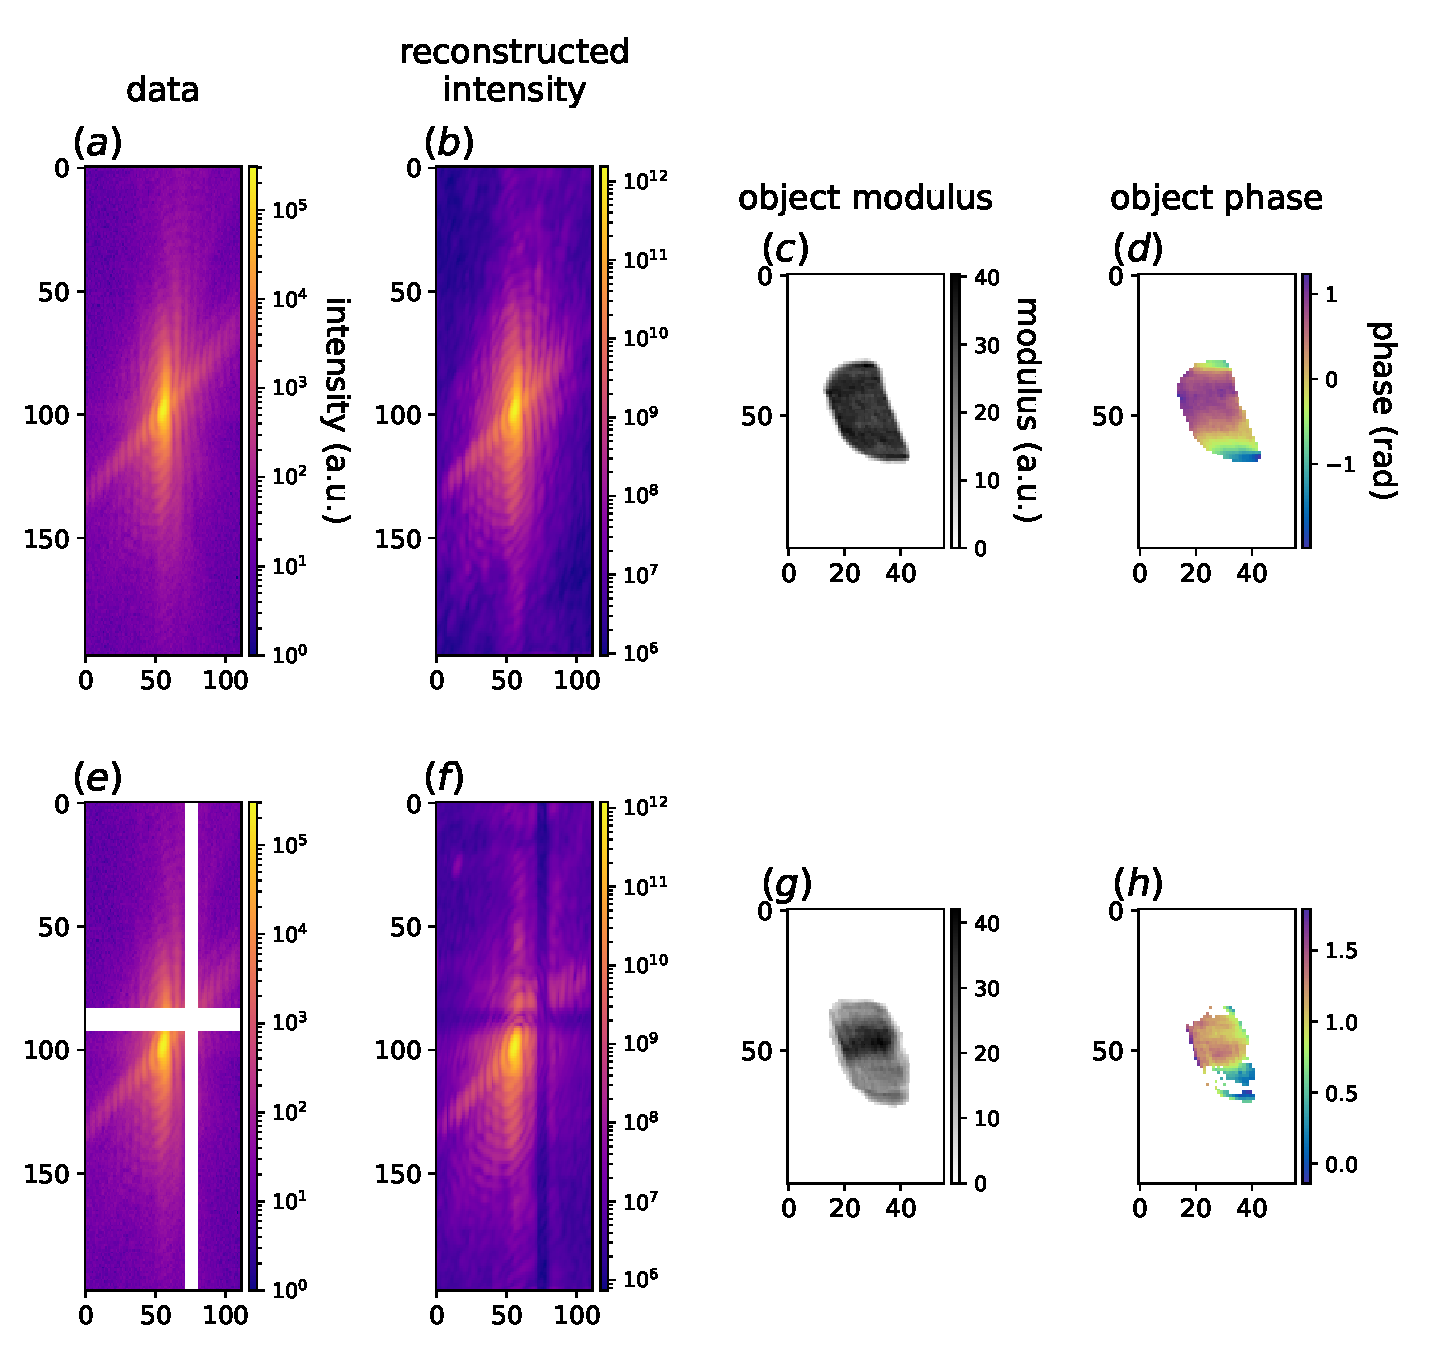
\includegraphics[width=\textwidth]{figures/Inpainting/gaps_intropdf.pdf}
    \caption{\textbf{Effect of detector gaps in BCDI reconstructions} 
    \textbf{(a)} The central slice of an experimental diffraction pattern. \textbf{(b)} The same slice of the diffracted
    intensity calculated from the retrieved object. \textbf{(c - d)} slice of the modulus and phase respectively of the particle
    obtained from the phasing of the gap-less dataset. \textbf{(e)} Same slice as in \textbf{(a)} with an artificially added
    9 pixel-wide, cross-shaped gaps to mimic the detector's ones. \textbf{(f)} The same slice of the diffracted
    intensity calculated from the retrieved object when not masking the gap regions. \textbf{(h - g)} slice of the modulus and phase respectively of the particle
    obtained from the phasing of the gap-affected dataset. The distortions caused by the gaps are evident. Note that for 
    this figure an extreme, but explanatory case of large gaps near central peak of a low-oversampled data was illustrated. }
    \label{fig:gap_intro}
    \end{figure}


It follows that the reliability of the reconstructions in this case is 
compromised as the strain distribution can be deeply affected by the artifacts. A good practice during standard BCDI experiments
is to avoid the gaps by moving the detector if possible. However, this tends to be problematic for the case of high-resolution BCDI, 
i.e. when the diffraction pattern measurement extends to higher q-values, thus covering more than one sensing 
chip and necessarily crossing a gap region. Under these circumstances it becomes important to reduce the amount of
artifacts deriving from the gaps. 


\section{State of the art}\label{sec:InpStateArt}

Here we will discuss the current strategies employed to treat the detector gaps. As someone could argue the simplest,
yet not practical, solution would be to slightly move the detector sideways and acquire a second full scan with the
gap hiding a different region of the same Bragg peak, and then merge the two measurements into a single gap-less one. 
This would at least double the acquisition time making it, de facto, not an option during standard experiments. 

The PyNX software, routinely used for the BCDI phase retrieval at ID01, allows the user to define a mask of the gap 
regions and ignore those pixels during the execution. This improves the quality of the reconstruction, 
but one can still notice the presence of oscillations appearing in both the object's modulus and phase.
The origin of these artifacts can be found in the diffracted intensity calculated from the reconstructed particle as 
one can clearly see that the gap-regions is filled with non-physical high intensity (see Fig. \ref{fig:gap_intro_mask}(f))

\begin{figure}[h]
    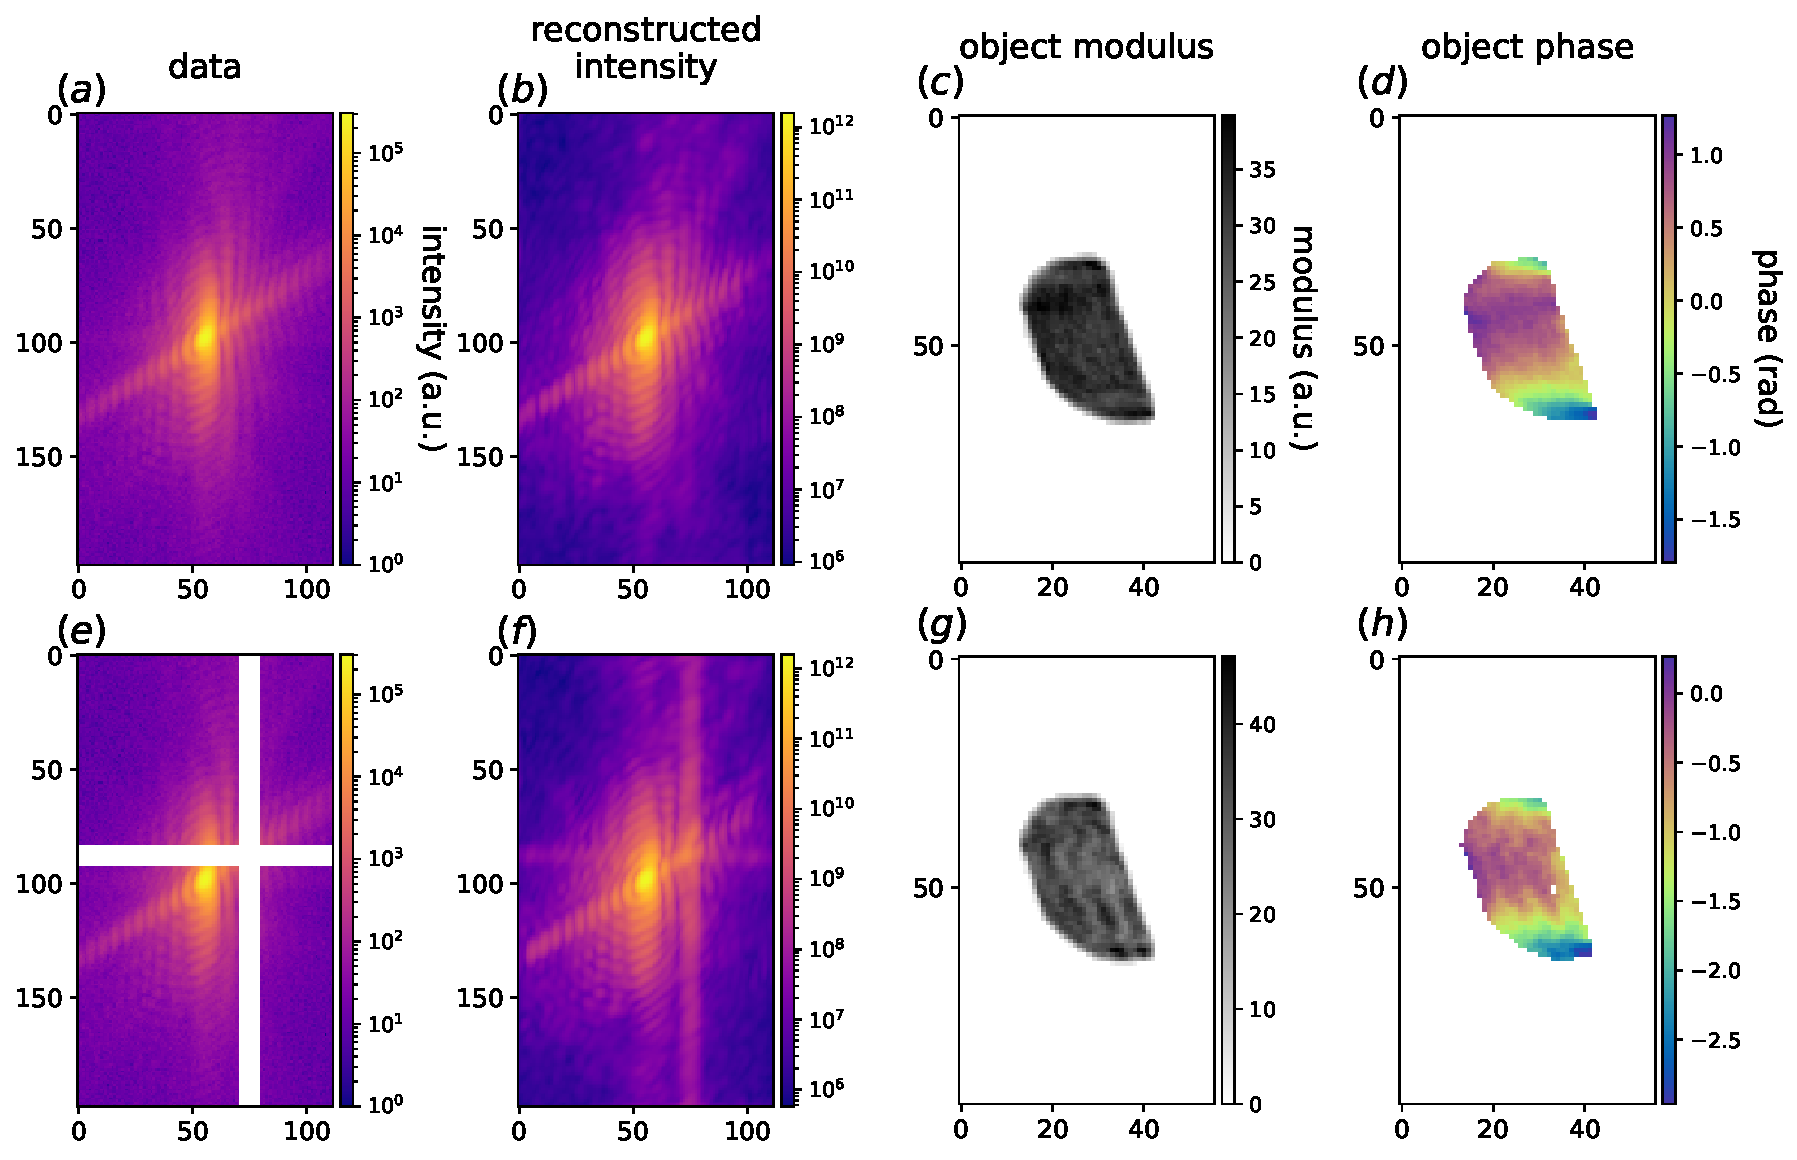
\includegraphics[width=\textwidth]{figures/Inpainting/gaps_mask.pdf}
    \caption{\textbf{Masking the gap region during phasing} 
    \textbf{(a)} The central xz slice of an experimental diffraction pattern. \textbf{(b)} The same slice of the diffracted
    intensity calculated from the retrieved object. Comparing this figure with \ref{fig:gap_intro}\textbf{(b)} one can see that
    when excluding the gap region from the phasing with a mask, the calculated intensity shows bright non-physical streaks 
    instead of the gaps. \textbf{(c - d)} xz slice of the modulus and phase respectively of the particle obtained from the 
    phasing of the gap affected data with a mask of the gap regions. Despite the much higher quality of the reconstruction, 
    one can notice some oscillatory artifacts appearing in both the modulus and the phase of the retrieved object. }
    \label{fig:gap_intro_mask}
\end{figure}

Methods relying on compressive sensing and TV regularization were proposed by He in \cite{He2015} and Malm 
\cite{Chushkin2025} respectively. Another, more invasive, option is to \textit{fill} these gaps with an estimate of 
the intensity distribution that would be there, before the phase retrieval. The task of filling gap in images is usually 
referred to as ``inpainting''.


\subsection{Background on Image Inpainting Research}
 
Computational image inpainting has been widely studied in the field of photography and imaging for many years \cite{Elharrouss_2019,reviewInpainting2021}. 
The inpainting problem can be defined as the task of using known information extractable from the image, to repair
the parts where this information is missing, where for known information the colors, the textures and the semantic features
are intended. In the history of image inpainting a clear-cut can be observed when deep learning methods have started to be employed.
For traditional inpainting, different techniques have been explored, from the texture synthesis methods pioneered by Efros and 
Leung \cite{Efros1999} to the use of PDEs as Navier-Stokes equations proposed by Bertalmio \textit{et al.} \cite{BertalmioNavierStokes}
and then again from sparse representations \cite{Mairal_sparse} to hybrid methods combining variational and statistical methods \cite{CedricAllene}

More recently, Deep Learning models, headed by Convolutional Neural Networks (CNN), have taken the place of more traditional 
methods as they can attain higher accuracy for more complex inpainting tasks. By undergoing a  
training process, CNNs can ``learn'' to recognize and reproduce the semantic features of the training dataset, and thus
leverage them during inference as additional information beside the colors and textures of the specific image to restore. 
As we have seen in Chapter \ref{chap:dl_theory}, the typical CNN architecture for image generation consists of an encoder, which
retains the features of the input image and compresses them into a lower dimensional latent space, and a decoder, which
is responsible for the generation of the output image starting from the latent space. The model is then trained according 
to a loss function that pushes the model's predictions to be close to a given ground truth reference. 
In some cases, the loss function can be replaced by another CNN that is trained to discriminate true images from the ones
predicted by the model. These complementary networks are known as Generative Adversarial Networks (GAN), firstly 
proposed by Goodfellow \textit{et al.} \cite{goodfellow2014generativeadversarialnetworks}, and have also been used for 
image inpainting (e.g. \cite{gan_inpainting}). 

Since reviewing the vast amount of works about CNN for image inpainting is beyond the scope of this thesis and for more 
information, we redirect the reader to the reviews written by Elharrouss \textit{et al.}, Xiang{et al.} and  Xu 
\textit{et al.} \cite{reviewInpainting2021,DL_InpaintingReveiw2023_0, reviewInpaintingDL2023}. For what concerns the application of DL based 
inpainting for scientific imaging, early works date back to 2018 as in the case of Sogancioglu \textit{et al.} for X-ray 
human chest 2D radiographic images \cite{sogancioglu2018chestxrayinpaintingdeep} and to 2020 for 2D microscopic images \cite{microscopic_inpainting_2020}.
A couple of years later Tanny Chavez and coauthors published a paper comparing the performance of different CNN models 
for the inpainting of 2D X-ray diffraction images \cite{chavez_comparison_2022}. The work is precisely addressing the 
gap problem for X-ray detectors used for powder diffraction measurements and is awarding U-Net and Mixed Scale Dense (MSD) 
models for the best performance on experimental data. The DL models outperform interpolations obtained with biharmonic functions
across 7 and 17 pixel-wide gaps. This work has been of inspiration for the design of our DL model for BCDI gaps inpainting.
In the same year, another work on DL based inpainting for X-ray detector gaps was published by Alfredo Bellisario 
and coauthors \cite{bellisario_noise_2022}. The authors tested a U-Net-like model on the inpainting of 2D simulated, noiseless
coherent diffraction patterns against gaps of different sizes (2 to 20 pixels) along the central row. The gaps were 
placed such that the center of the peak was covered, a choice that, as we will see later, yields better results than 
predictions on peripheral areas. To our knowledge, at the time of writing, no other works about deep learning based inpainting
for X-ray detector gaps are present in the literature. \\

% It is worth mentioning a different way, other than DL, to address the more general problem of missing data in CDI 
% techniques, and more specifically the \textit{artifacts} deriving from it, was recently proposed by Malm 
% and Chushkin \cite{Chushkin2025}. Here, a revised version of the RAAR algorithm including a Total Variation regularization 
% is shown to reduce the oscillatory artifacts caused by missing data during PR.  

\section{Model design: 2D case}\label{sec:model}

For simplicity, I have begun with the 2D case, using simulated diffraction patterns and inpainting randomly placed 
vertical gaps of different width. First, a training set of simulated data was created, composed of pairs of gap-affected 
images and corresponding gap-free ground truths, then a U-Net-like model was built and trained in a supervised fashion.

\subsection{Dataset creation}\label{sec:dataset_creation2D}

The creation of training datasets of simulated 2D BCDI patterns for both the gap-inpainting and phase retrieval tasks has followed the procedure
described in this paragraph.\\
First, once the size of the array was chosen, a randomly shaped polygon was created in the center using 
\texttt{scipy.spatial.ConvexHull} function. This guarantees the object to have a compact support with homogeneous electron 
density as assumed for BCDI. Subsequently, a random phase field of the same size with variable phase range and correlation 
length was generated thus the complete complex object was formed.

In order to make the object more realistic a Gaussian filter and Gaussian - correlated noise \cite{Gaussian_noise1984} 
have been applied to the 
object's modulus, to smoothen the edges and simulate real cases respectively. At this point the object was resized 
to the shape required to match the chosen oversampling ratio and the 2D Discrete Fourier Transform was computed. Finally, 
Poisson noise was added to the diffraction patterns with different magnitudes to simulate 
various X-ray flux conditions (see Fig.\ref{fig:2D_dataset_creation}). \\
Datasets contain a number of diffraction patterns in the order of thousands and for each of them the random variables 
have been varied as well as the oversampling ratios. In the datasets for the training of phase retrieval models (presented 
later in Chapter \ref{chap:phase_retrieval}) , 
the reciprocal space phase corresponding to each diffraction pattern was saved as well and used as ground truth label. 
For inpainting tasks a randomly located vertical gap mask was created and applied to the intensity data. In some cases 
cross-shaped gaps were added instead to simulate the experimental condition of the Bragg peak in the vicinity of the 
corner of the sensing area. The size of the gaps was chosen to be consistent across the dataset and four different 
cases were studied (3px, 6px, 9px, 12px). Fig.\ref{fig:2D_dataset_creation}. 

\begin{figure}[h]
    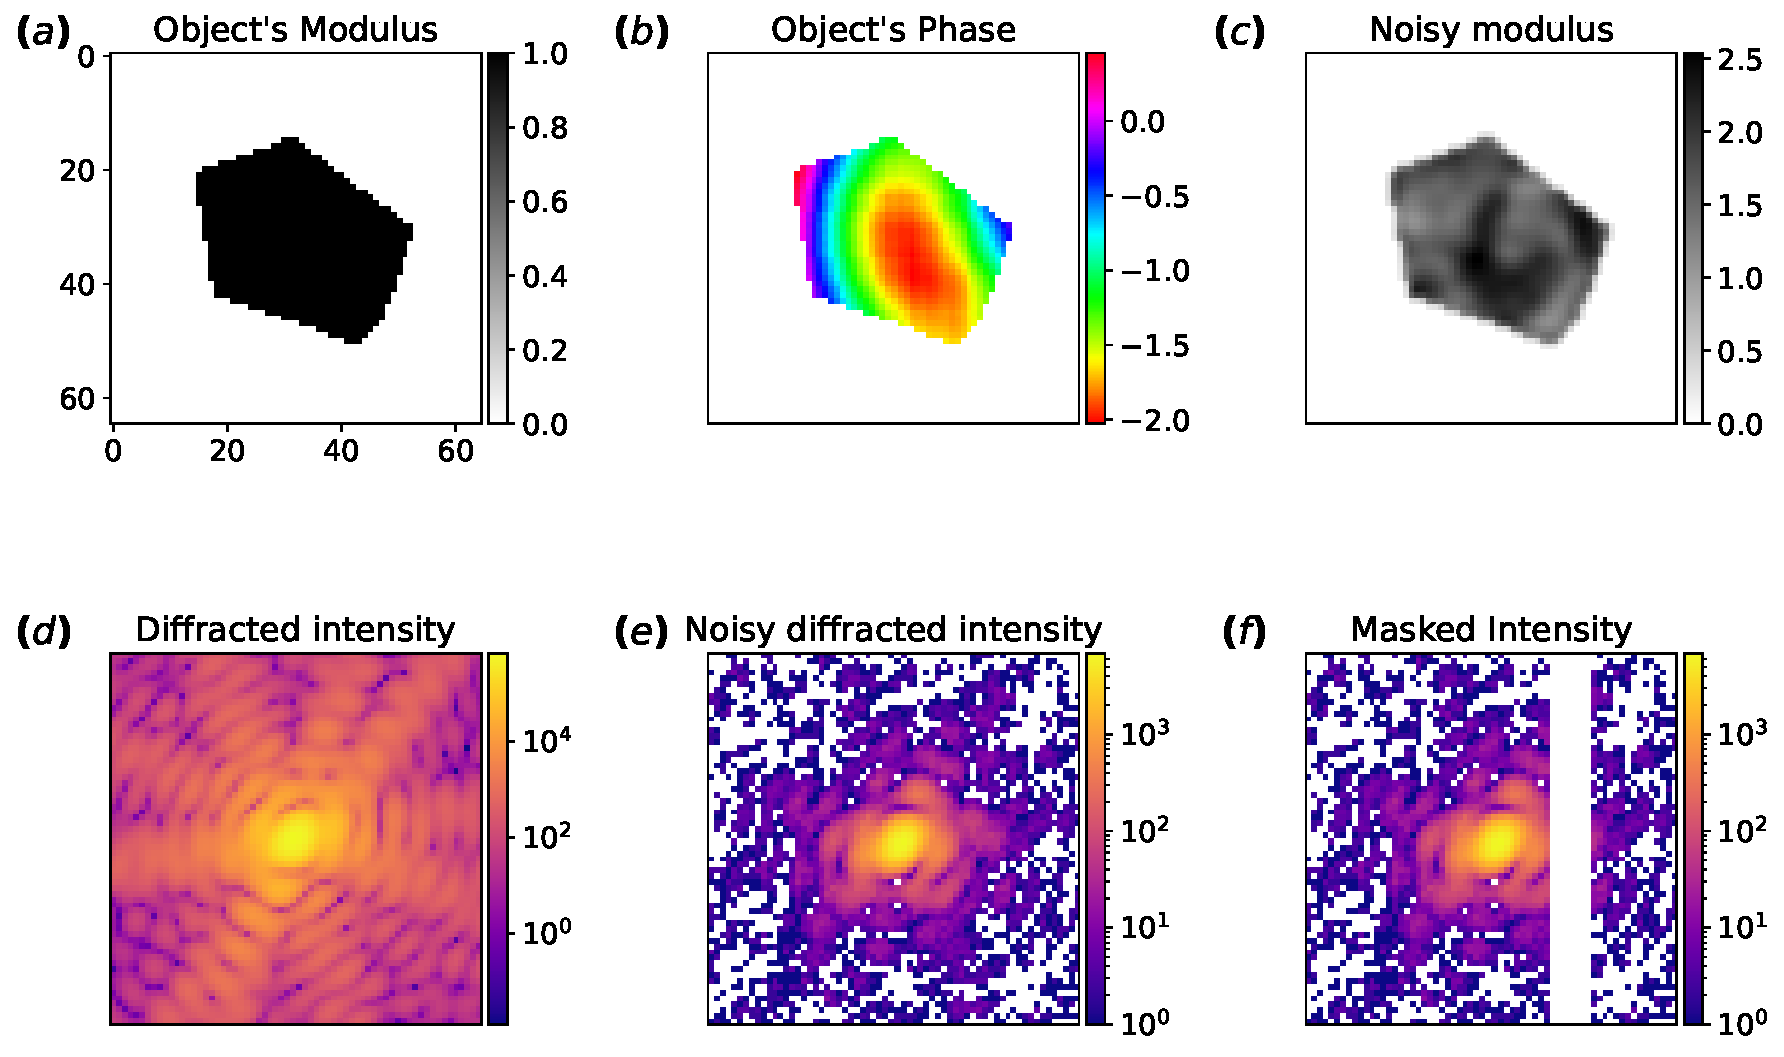
\includegraphics[width=\textwidth]{figures/Inpainting/2D_dataset_creation.pdf}
    \caption{\textbf{Steps for the simulation of a single 2D diffraction pattern} 
    \textbf{(a)} Simulated modulus of a 2D object with random shape and compact support. The object is padded with 
    zeros to match the chosen oversampling ratio. \textbf{(b)} Simulated object's phase
    \textbf{(c)} Object's modulus after smoothening the edges and adding random Gaussian noise. \textbf{(d)} Squared modulus of the Fourier Transform
    of the complex object (in log scale).
    \textbf{(e)} Poisson noise is added to the simulated diffracted intensity. \textbf{(f)} A 6 pixel-wide
    vertical gap is added to the diffracted intensity at a random position.}
    \label{fig:2D_dataset_creation}
\end{figure}


\subsection{2D Model design}

The 2D model that I have implemented is a U-Net that takes in input batches of 32 simulated BCDI patterns affected 
by both vertical and cross-shaped gaps. Each diffraction pattern was transformed into logarithmic scale to enhance the 
spatial features and then normalized between 0 and 1. This normalization was proven to be convenient to any DL model \cite{efficientBackProp}.
Regarding the logarithmic transformation, it is important to notice that in order to avoid problems for zero intensity
values, the $\log(I+1)$ was taken.
The shape of each image was chosen to be of $128\times128$ pixels. The encoder of part of the models was built as follows. 
The inputs go through five convolutional blocks 
inside each of which a convolutional layer, a Leaky ReLU activation function and a MaxPooling operation are applied. 
The feature map's size is therefore reduced down to $2\times2$ while the channel dimension is brought up to 768 filters, 
and the kernel size is kept at $3\times3$. At the end of the encoder the feature map passed to the decoder is a 
$(32,2,2,768)$ tensor.
The decoder, mirroring the encoder, is composed of five blocks inside each of which there is a transposed convolutional layer
that upsamples the feature maps (stride = 2) and a Leaky ReLU activation function. Skip connections connecting each encoder block
to its corresponding shape-like decoder block have been implemented as well. This measure has proven to be beneficial 
for the information flow between encoder-decoder \cite{li_visualizing_2017}. The last activation layer of the model is 
a sigmoid function that guarantees an output bounded between 0 and 1. \\ 

A simple Mean Squared Error (MSE) was used as loss function inside the gap region only, training 
the model on 12'000 diffraction patterns over 10 epochs, with ADAM optimizer and a learning rate of $10^{-4}$. 
The Mean Absolute Error (MAE) and the Structural Similarity Index Measure (SSIM) \cite{ssim} loss functions were 
tested as well and the corresponding results obtained after the same training were compared.
Here in Fig. \ref{fig:loss_comparison_inpainting} we report the comparisons for the 9 pixel-wide gap on a test simulated diffraction
pattern. The accuracy scores were calculated using the Pearson Correlation Coefficient (PCC).

\begin{equation}
    PCC = \frac{\sum_{i\in \text{gap}}(\textbf{I}_i^{\text{true}} - 
    \langle \textbf{I}^{\text{true}}\rangle)(\textbf{I}_i^{\text{pred}}-
    \langle\textbf{I}^{\text{pred}}\rangle)}{\sqrt{\sum_{i\in \text{gap}}^{}(\textbf{I}_i^{\text{true}} - 
    \langle \textbf{I}^{\text{true}}\rangle)^2}\sqrt{\sum_{i\in \text{gap}}^{}(\textbf{I}_i^{\text{pred}}-
    \langle\textbf{I}^{\text{pred}}\rangle)^2}},
        \label{eq:accuracy}
\end{equation}

Where \textbf{I} is the intensity inside the gap. The PCC measures the linear correlation between two sets of data, 
and it is naturally normalized between -1 and 1 for which the two datasets are said to be linearly correlated. On the 
contrary the 0 value implies uncorrelated sets. 

\begin{figure}[h]
    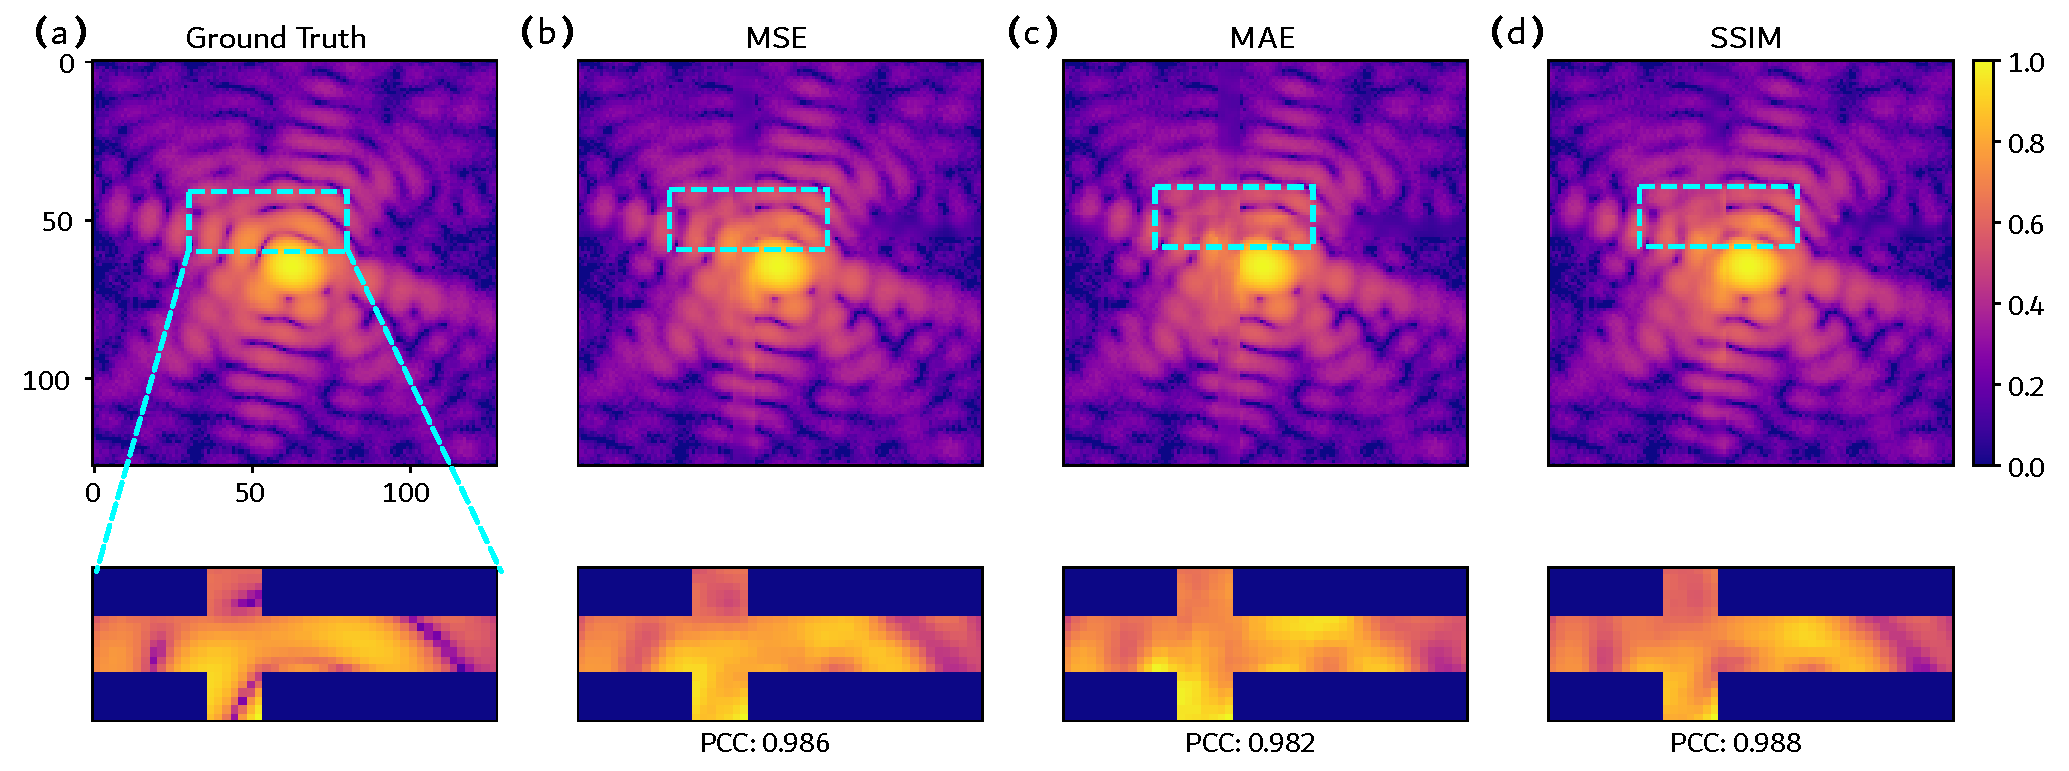
\includegraphics[width=\textwidth]{figures/Inpainting/loss_comparison.pdf}
    \caption{\textbf{Comparison of different losses} Results on a test simulated diffraction pattern for the inpainting 
    of a 9 pixel-wide cross-shaped gap produced by the same U-Net model trained for 10 epochs with different loss functions. 
    \textbf{(a)} Shows the ground truth. \textbf{(b)} The prediction of the model trained with the MSE, \textbf{(c)} 
    with the MAE, \textbf{(d)} with the SSIM. Corresponding accuracy scores calculated with the Pearson Correlation 
    Coefficient (PCC) are shown as well. While MAE fails to recover the oscillations, SSIM yields better results.}
    \label{fig:loss_comparison_inpainting}
\end{figure}

In the light of these results, the MAE metric was discarded and the sum of MSE and SSIM adopted instead. 
Finally, another term that computes the MSE between the \textit{gradients} of the ground truth and predicted intensity inside
the gap region was added in the definitive loss function.\\

Once established what was considered the best loss function, different models have been explored . 
Following the work of Chavez \textit{et al.} mentioned above (\cite{chavez_comparison_2022}), a 
Mixed-Scale Dense Network (MSD-Net) was used \cite{MSD_Pelt2017}. The advantage of this type of network is the significant reduction of trainable
parameters, and the use of \textit{dilated} convolutions with respect to U-Net ones. While the former property guarantees
faster training and lower chances of overfitting, the latter enhances the capture of long-range correlations. Moreover, 
in an MSD-Net, the image's spatial dimensions are kept constant throughout the whole network as no downsampling nor upsampling is made.
The MSD-Net consists of sequential blocks in each of which the input is transformed by two different 
convolutional layers with growing dilation rates. Each output of the convolutional layers is concatenated to the input 
feature map and the result is passed to the following block. While the kernel size is kept constant to $3\times3\times3$ pixels
the dilation rate increases linearly from 1 to 30. The last layer is a sigmoid function as well as for the U-Net. 
The total number of trainable parameters is of the order of 320'000, two orders of magnitude lower than the U-Net.
\\
In order to combine the hierarchical dimensionality reduction of the U-Net with the fine-features capturing of the MSD-Net 
we have implemented a modified U-Net that adopts dilated convolutions inside the first three encoder blocks. In particular, 
they return the input tensor concatenated with the outputs of four dilated convolutional layers computed
from the input. Dilation rates of (16,8,4,2), (10,5,3,1) and (5,3,2,1) were chosen respectively. As the MaxPooling 
operation down-samples the feature maps into smaller sizes, we limited the dilated convolutions to the first three 
blocks. Moreover, they were used in the encoder layers only as they are mostly used for feature extraction \cite{dilated_conv}.
The characteristics of each model are summarized in form of pseudo - code in Table \ref{tab:model_comparison}.
\\

The three different models have been trained with a combined loss function (MSE + SSIM + MSE on the gradients) on the 
same training dataset for 10 epochs each.  The results showed poor performances of the MSD-Net with respect to the two 
U-Nets. Slightly higher accuracy was achieved by the modified U-Net (see Fig. \ref{fig:models_comparison}). 

\begin{figure}[h]
    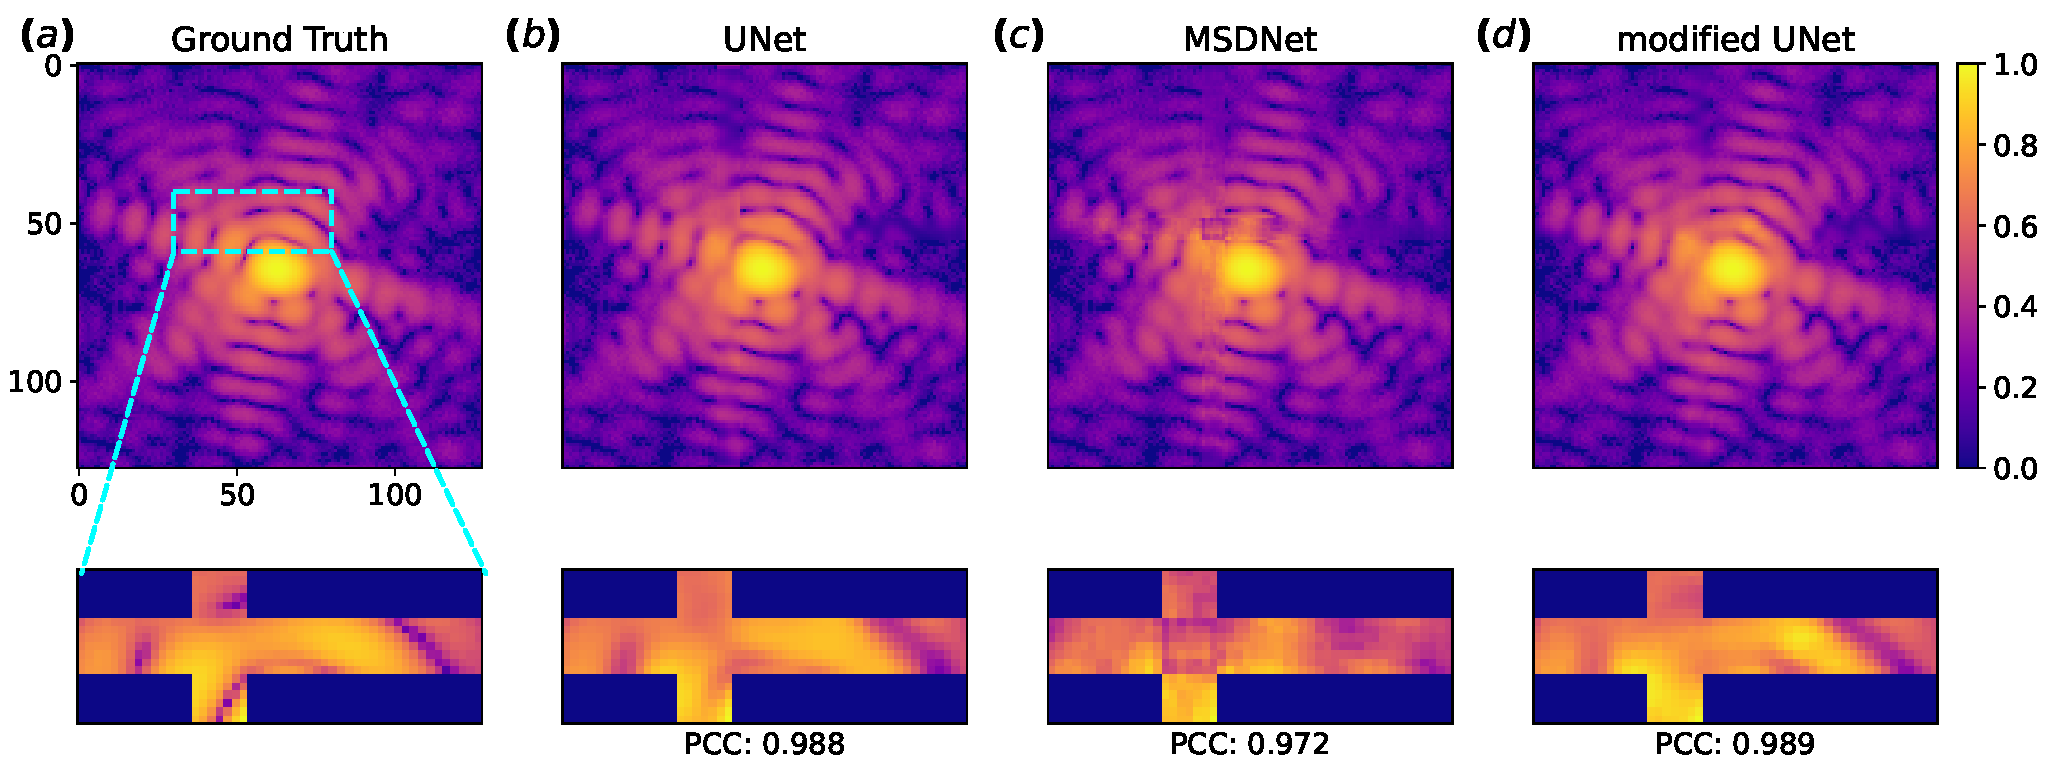
\includegraphics[width=\textwidth]{figures/Inpainting/model_comparison.pdf}
    \caption{\textbf{Comparison of different models} Results on a test simulated diffraction pattern for the inpainting 
    of a 9 pixel-wide cross-shaped gap using three different models trained with the same loss function.
    \textbf{(a)} Shows the ground truth. \textbf{(b)} The prediction of the U-Net, \textbf{(c)} 
     of the MSD-Net, \textbf{(d)} of the modified U-Net. Corresponding accuracy scores calculated with the Pearson Correlation 
    Coefficient (PCC) are shown.}
    \label{fig:models_comparison}
\end{figure}


\begin{table}[h!]
    % \small 
    %  or 
    \scriptsize
    \centering
    % \resizebox{\textwidth}{!}{%
    \begin{tabular}{|>{\centering\arraybackslash\bfseries}p{1.2cm}|p{4.5cm}|p{4.5cm}|p{4.5cm}|}
    \hline
     & \textbf{U-Net} & \textbf{MSD-Net} & \textbf{U-Net\_mod} \\ \hline
    block1 & 
    \begin{lstlisting}[basicstyle=\tiny\ttfamily, xleftmargin=-1em]
    def encoder_block(x_input, num_filters, ker):
        s = Conv2D(num_filters, ker,'leaky_relu')(x_input)
        x = MaxPool2D(2)(s)
        return x, s
    \end{lstlisting} 
    & \begin{lstlisting}[basicstyle=\tiny\ttfamily, xleftmargin=-1em]
    def MSD_block(x, in_channels, dilations,kernel_size=3):  
        if isinstance(dilations, int):  
            dilations = [(j % 10) + 1 for j in range(dilations)]  
        out_channels = in_channels + len(dilations)  
        for d in dilations:  
            x1 = Conv2D(out_channels//2,kernel_size,1, dilation_rate=dilation, 'same', 'leaky_relu')(x)
            x = tf.concat([x1,x] ,axis = -1)
        return x, out_channels
    \end{lstlisting} 
    &
    \begin{lstlisting}[basicstyle=\tiny\ttfamily, xleftmargin=-1em]
    def encoder_block_mod(x_input, ker, num_filters, rate):
        f = num_filters // 4
        s = tf.concat([x_input] + [Conv2D(f, ker, dilation_rate=r, 'leaky_relu')(x_input) for r in rate], axis=-1)
        return MaxPool2D(2)(s), s
    \end{lstlisting} \\ \hline
    block2 
    &
    \begin{lstlisting}[basicstyle=\tiny\ttfamily, xleftmargin=-1em]
    def decoder_block(x_input, num_filters, ker, skip_input = None):
    
        if skip_input is not None:
            x_input = Concatenate()([x_input, skip_input])
            
        x = Conv2DTranspose(num_filters, ker, strides=2, 'leaky_relu')(x_input)
        return x
    \end{lstlisting} 
    & 
    &
    \begin{lstlisting}[basicstyle=\tiny\ttfamily, xleftmargin=-1em]
    def decoder_block(x_input, num_filters, ker, skip_input = None):
    
        if skip_input is not None:
            x_input = Concatenate()([x_input, skip_input])
            
        x = Conv2DTranspose(num_filters, ker, strides=2, 'leaky_relu')(x_input)
        return x
    \end{lstlisting} \\ \hline
    
    body & 
    \begin{lstlisting}[basicstyle=\tiny\ttfamily, xleftmargin=-1em]
        x, s1 = encoder_block(inputs, 48,3)        
        x, s2 = encoder_block(x, 96,3)             
        x, s3 = encoder_block(x, 192,3)           
        x, s4 = encoder_block(x, 384,3)           
        x, s5 = encoder_block(x, 768,3)          
    
        x = Conv2D(1536,3, 'leaky_relu')(x) 
    
        x = decoder_block(x,768,3)
        x = decoder_block(x,384,3, s5)
        x = decoder_block(x, 192,3,s4)
        x = decoder_block(x, 96,3,s3)
        x = decoder_block(x, 48,3,s2)
        
        x = Conv2D(24,5,'leaky_relu')(x) 
        x = Conv2D(12,5,'leaky_relu')(x)
        x = Conv2D(6,5,'leaky_relu')(x)
        
        out = Conv2D(1,5,'sigmoid')(x)
    \end{lstlisting} 
    & 
    \begin{lstlisting}[basicstyle=\tiny\ttfamily, xleftmargin=-1em]
        x,out_ch = MSD_block(inputs,1,[1,2])
        x,out_ch = MSD_block(x,out_ch,[3,4])
        ...
        ...
        x,out_ch = MSD_block(x,out_ch,[31,32])
        out = Conv2D(1,3,'sigmoid')(x)
    \end{lstlisting} 
    &
    \begin{lstlisting}[basicstyle=\tiny\ttfamily, xleftmargin=-1em]
        x, s1 = encoder_block_mod(inputs,3,48,[16,8,4,2])   
        x, s2 = encoder_block_mod(x,3, 96,[10,5,3,1])       
        x, s3 = encoder_block_mod(x,3, 192,[5,3,2,1])           
        x, s4 = encoder_block(x, 384 ,3)            
        x, s5 = encoder_block(x, 768, 3)                    
        
        x = Conv2D(1536,3,'leaky_relu')(x)
        
        x = decoder_block(x,768,3)    
        x = decoder_block(x,384,3,s5)  
        x = decoder_block(x,192,3,s4)  
        x = decoder_block(x,96,3,s3) 
        x = decoder_block(x,48,4,s2)  
    
        x = Concatenate()([x, s1])
        x = Conv2D(24,5,'leaky_relu')(x) 
        x = Conv2D(12,5,'leaky_relu')(x)   
        x = Conv2D(6,5,'leaky_relu')(x)
    
        out = Conv2D(1,3,'sigmoid')(x)
    \end{lstlisting} \\ \hline
    parameters & 31,827,673 & 322,458 & 32,652,337 \\ \hline
    \end{tabular}
    \caption{Comparison of U-Net, MSDNet, and U-Net\_mod components.}
    \label{tab:model_comparison}
\end{table}

We conclude here the introductory studies on 2D simulated data. These preliminary tests allowed to explore 
different DL architectures and loss functions and select the optimal choices for the inpainting of BCDI detector
gaps. 

\subsection{Accuracy VS Gap position}

Before moving to the 3D case, it is worth spending a few words on the assessment of the DL model upon different conditions.
Namely, the accuracy as function of the position of the gap inside the diffraction pattern and as a function of the oversampling ratio.
For the first test 150 2D diffraction patterns were simulated starting from random particles shapes, random oversampling ratios
and Poisson noise intensity. For each diffraction pattern a vertical 9 pixel-wide gap was placed at all positions
from left to right, then the DL prediction and corresponding accuracy score when compared to the ground truth were calculated. The 
accuracy was again calculated with the Pearson Correlation Coefficient. This score was then averaged for each 
gap position, over the 150 diffraction patterns and the result was plotted as a function of the gap position. Fig. \ref{fig:accVSpos} 
shows the resulting curve that clearly highlights that the model performs better in regions with high intensity. 
This can be qualitatively explained: (i) central pixels contain larger spatial features both because of the 
nature of the Bragg peak, and because of the lower noise level. This makes it easier for the model as it reduces the 
complexity of the prediction. (ii) As we move away from the center of the Bragg peak, the Signal to Noise Ratio (SNR) 
decreases, along with the \textit{density of signal}. High accuracy scores in these regions would require the model to be 
able to predict noise correctly which is by definition impossible as it is an uncorrelated random process. One could argue 
that the accuracy curve would follow the statistical distribution of the gap positions inside the DL model training dataset.
However, each mask has been applied at a position drawn from a discrete uniform probability function spanning the full
data size, so can be excluded. 

\begin{figure}[h]
    \centering
    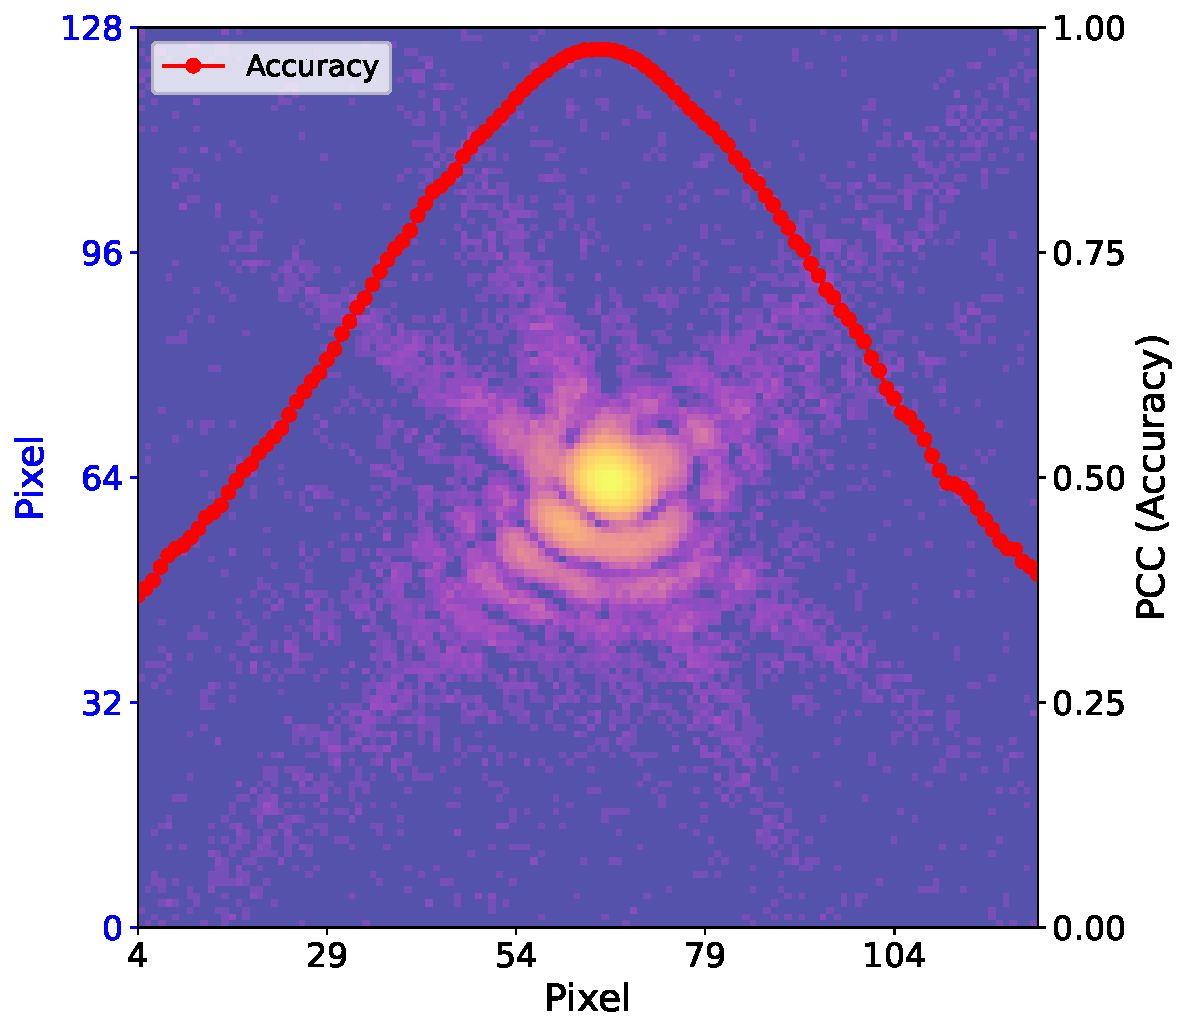
\includegraphics[width=.7\textwidth]{figures/Inpainting/2D_acc_pos.pdf}
    \caption{\textbf{(Accuracy VS Gap position)} Average Pearson Correlation Coefficient calculated over 150 
    9 pixel-wide vertical predicted gaps for each position of the gap inside the diffraction patterns. The model 
    shows higher accuracies when the gap masks high intensity regions.}
    \label{fig:accVSpos}
\end{figure}

To conduct the second test, 150 diffraction patterns were simulated for the same particle varying gradually the oversampling
ratio (see Sec.\ref{sec:oversampling}) between 2 and 6. For each image a 9 pixel-wide vertical gap was then applied 
at all $X$ positions and the DL prediction was computed. The accuracy scores have been averaged for each prediction 
in the same image and plotted against the oversampling 
(Fig. \ref{fig:accVSovs}). As expected from the previous discussions, the model performs better for larger oversampling ratios, 
because of the bigger size of the features with respect to the gap width and because of the more uniform \textit{density of signal}.
It is worth clarifying that, for a given particle, the total amount of intensity in the
diffraction patterns is in principle constant regardless of the oversampling ratio as it is fixed by Parseval's theorem
\footnote{Interpreted also as an energy conservation law, Parseval's theorem states that $ \int |f(x)|^2 dx = \int |\mathcal{F}\{f(x)\}|^2 dk$. 
In other words, the overall amount of signal is constant in direct space as in Fourier space.}.
However, if the size of the dataset is kept fixed for different oversamplings, the effect is the same of a zoom lens
that increases or reduces the field of view. Therefore, while for low oversampling ratios the full peak is recorded, 
for higher ones the peak is cropped, and less intensity is present in the image.

This effect, coupled with the typical radial
intensity decay of Bragg peaks and of Poisson noise, reduces the \textit{density of signal} in largely oversampled BCDI 
patterns. Here the \textit{density of signal} refers to the amount of information per pixel, which becomes smaller and more uniform. 
On the contrary, for low oversampling ratio the \textit{density of signal} is less uniform as it is high inside bright 
regions (a lot of information concentrated in few pixels) and low in noisy regions far from the peak. It follows that 
in order to properly assess the accuracy against the oversampling ratio one should consider diffraction patterns over 
the same extent in $q$-space, thus changing the size of the images. This more accurate evaluation was carried out for 
the 3D case and can be found in the next section.

\begin{figure}[h]
    \centering
    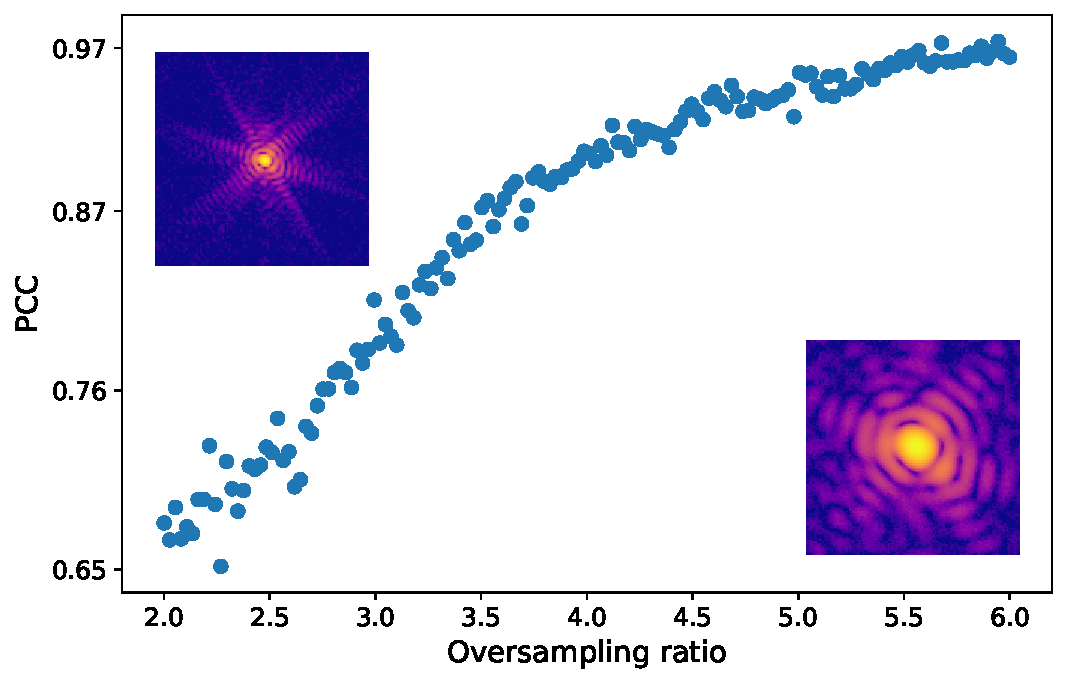
\includegraphics[width=.7\textwidth]{figures/Inpainting/2D_acc_ovs.pdf}
    \caption{\textbf{(Accuracy VS Oversampling ratio)} Average Pearson Correlation Coefficient calculated over 280
    9 pixel-wide vertical predicted gaps for each position of the gap inside the diffraction patterns. The model 
    shows higher accuracies for high oversampling ratios.}
    \label{fig:accVSovs}
\end{figure}

\section{3D case - Patching approach}\label{sec:patching}

When considering the 3D case, and especially the experimental conditions, there are a few practical issues that need
to be overcome. In fact, experimental BCDI datasets that are more often affected by a detector's gaps are necessarily large
datasets (e.g. $512\text{px} \times 512\text{px} \times N_{\text{rocking\_steps}}$ where $ N_{\text{rocking\_steps}}$ is of 
the order of hundreds of pixels in typical BCDI experiments). 
Training a U-Net like model for 3D images of that size is 
overly expensive in terms of computing memory and time. Moreover, a common problem with this type of architectures is that
the size of the images they can process is fixed by the first initialization. This means that one would need to resize, via 
binning or interpolation, the experimental datasets to the shape accepted by the DL model, and back to the original
shape after the inpainting. Besides the impracticality, these operations are not recommended as they induce further
modification and information loss to the original data. For these reasons a patching approach that 
loosens these constraints while preserving sufficiently high accuracies was considered. \\

The patching method exploits the regularity of the oscillations within BCDI datasets. The periodicity of the fringes 
in reciprocal space, peculiar property of this coherent diffraction technique, follows from the oversampling condition 
as it is given a product of the Fourier transform 
of an object less than half of the Fourier window containing the diffraction pattern. It can be observed by eye and 
in many cases makes the prediction inside a gap region intuitively possible starting from just a few neighboring pixels. 
In our case we have decided to work with 32 pixel-sided cubic sub-volumes (patches from now on) cropped out of entire diffraction 
patterns. Among the ``GPU-friendly'' tensor sizes \cite{nvidia_tensor_cores_optimization} we opted for 32 as a good trade-off
between amount of contained information and computing power required for training and inference. Moreover, this size is 
also greater than twice the size of the usual gap sizes and enough to catch several fringes in typical experimental 
oversampling conditions ($< 10$ usually). 

\subsection{Dataset creation}\label{sec:dataset_creation3D}
The training dataset consists of 50\% patches from experimental data and 50\% from simulated data.
The experimental measurements were acquired at the ID01 beamline of the ESRF during different beamtimes on different particles.
Namely, (i) Pt particles de-wetted on sapphire and YSZ (yttria–stabilized zirconia) with Winterbottom shape, 
measured under various temperatures and gas conditions, (ii) Pd and PdCe particles on glassy carbon, with
Wulff shape, measured in an electrochemical environment following hydrogen loading. (iii) Ni particles on sapphire undergoing
changes during $CO_2$ adsorption and (iv) ``cubic $CaCO_3$'' particles on glassy carbon.
\\
The synthetic diffraction patterns were instead simulated in three steps. The first step consisted in the creation of 
simulated 3D particles of different shapes (Winterbottom, Wulff, Cubic, Octahedral and random) using pre-existing scripts
developed by Dr. Dupraz and Dr. Bellec \cite{lim_convolutional_2021}. These codes allow the user to construct a cubic FCC
crystal of a given element, taking into account the inter-atomic potential, the atomic mass
and the lattice parameter. 

The final particle was finally obtained by "cutting" off atomic planes along given (or random)
directions, depending on the chosen shape. Only Gold nano-particles were simulated, and this is, in first approximation,
equivalent to any generic element as a different lattice parameter would just shift the Bragg peak to a different 
position in reciprocal space, with no significant alterations of the diffraction pattern itself.  
Each particle's configuration was then automatically saved in a LAMMPS-readable file. In a second stage,
energy relaxation using LAMMPS software for Molecular Dynamics was performed \cite{LAMMPS2022}. This step induces small displacements 
to the perfect lattice, especially near the surface and the substrate. In the last stage, the 3D diffraction pattern of a selected Bragg 
reflection was computed using PyNX scattering package \cite{pynx_scattering}. This software, optimized for GPU 
acceleration, produces a 3D representation of a selected Bragg peak using the kinematic sum.
It was then possible to adjust the parameters that control the oversampling ratio, the size of the array in which the 
Bragg peak was centered and the rotation of the $q$-space. In this case, 128 pixel-size cubic diffraction 
patterns were simulated and, in order to augment the training dataset, various oversampling ratios (from 2 to 5) and 
different rotations for each particle were selected.

As we have seen in Chapter \ref{chap:bcdi}, in the kinematic scattering 
approximation the energy of the incident X-ray does not alter the diffraction pattern if not as a ``zooming'' factor. 
It follows that simulating diffraction patterns for different X-ray energies for a fixed pixel size and distance results 
in different oversampling ratios. 

Before taking portions of these simulated BCDI patterns, Poisson noise was applied, randomly scaling the $\lambda$ parameter
for each image.


% \begin{figure}[h]
%     \centering
%     \begin{subfigure}{0.45\textwidth}
%         \centering
%         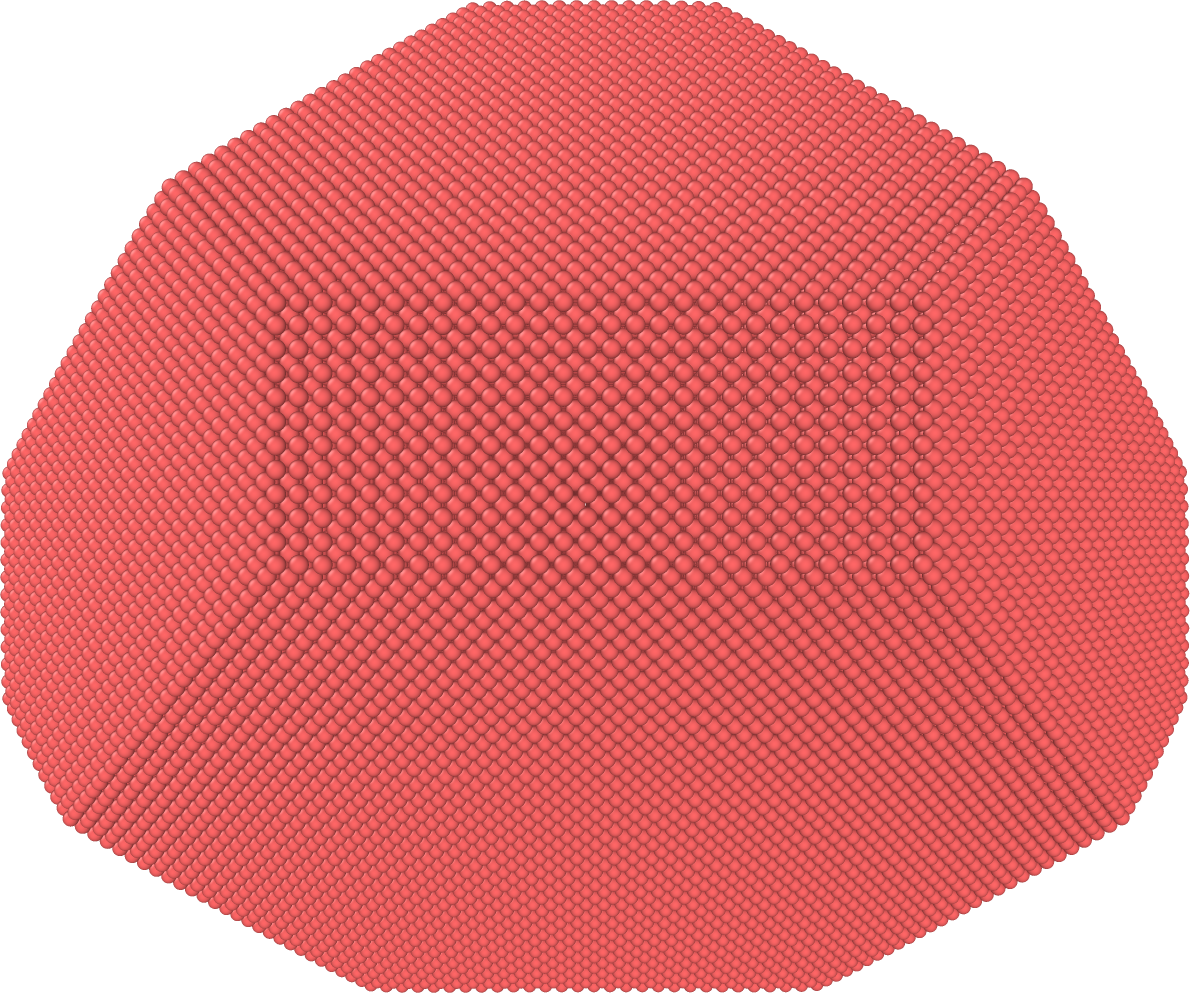
\includegraphics[width=\linewidth]{figures/Inpainting/crystal.png}
%         \caption*{}
%     \end{subfigure}
%     \hfill
%     \begin{subfigure}{0.45\textwidth}
%         \centering
%         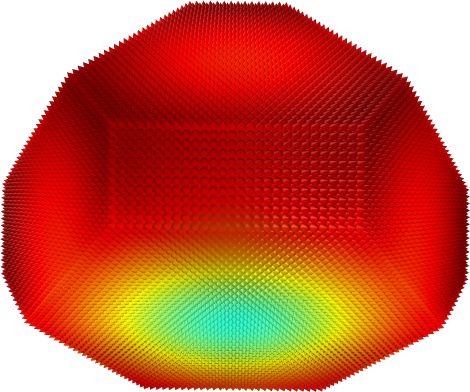
\includegraphics[width=\linewidth]{figures/Inpainting/displacement_field.png}
%         \caption*{}
%     \end{subfigure}
%     \caption{\textbf{Left}: Simulated Au particle with Winterbottom shape (134114 atoms). 
%     \textbf{Right}: Atomic displacement field of the same particle after LAMMPS energy relaxation. 
%     The typical distribution at the interface with the substrate is evident.}
%     \label{fig:comparison}
% \end{figure}

\begin{figure}[h]
    \centering
    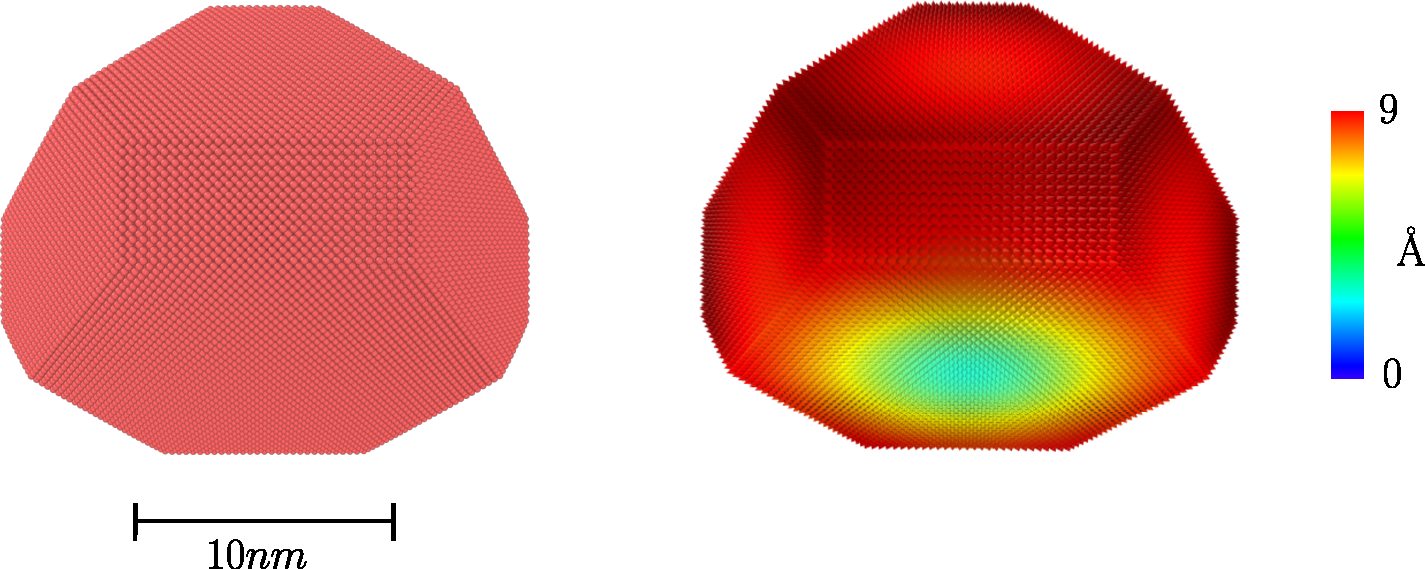
\includegraphics[width=\textwidth]{figures/Inpainting/ovitos.pdf}
    \caption{\textbf{Left}: Simulated Au particle with Winterbottom shape (134114 atoms). 
        \textbf{Right}: Atomic displacement field of the same particle after LAMMPS energy relaxation showing 
        the typical distribution at the interface with the substrate.}
     \label{fig:comparison}
\end{figure}

At this point, I proceeded with the extraction of patches taken at \textit{pseudo}-random locations inside each 3D pattern. 
The selection in fact was not totally random as the extraction of patches from the outer regions, far from the 
center of the peak was favored. There are mainly two reasons for this choice, namely (i) compensate the inherent uneven accuracy score against
the position of the gap (see Fig.\ref{fig:accVSpos}) by increasing the training data far from the center and (ii) emulate
as much as possible the experimental conditions, in which unavoidable gaps are typically far from the center of the peak.
For each sub-volume a 3D mask of the gap was created for different gap sizes (3,6,9,12 pixel-wide). The gap was placed 
vertically, in the center, along the third dimension, resulting in a ``empty slab''. Notice that, while in practice a 
gap may obscure the diffraction pattern at any position, it is unnecessary to consider other placements within a 
patch, since one can always select a patch symmetrically around the gap. Cross-shaped gaps were also 
included in the training dataset, with a population ratio of 1:5 compared to vertical gaps. They were created by 
adding a horizontal gap at a random height to an existing vertical gap (Fig. \ref{fig:patches_method}).
The final training dataset consisted of 30'000 $32\times32\times32$ pairs of patches, with gap and ground truth, 
created as described above. 

\begin{figure}[h]
    \centering
    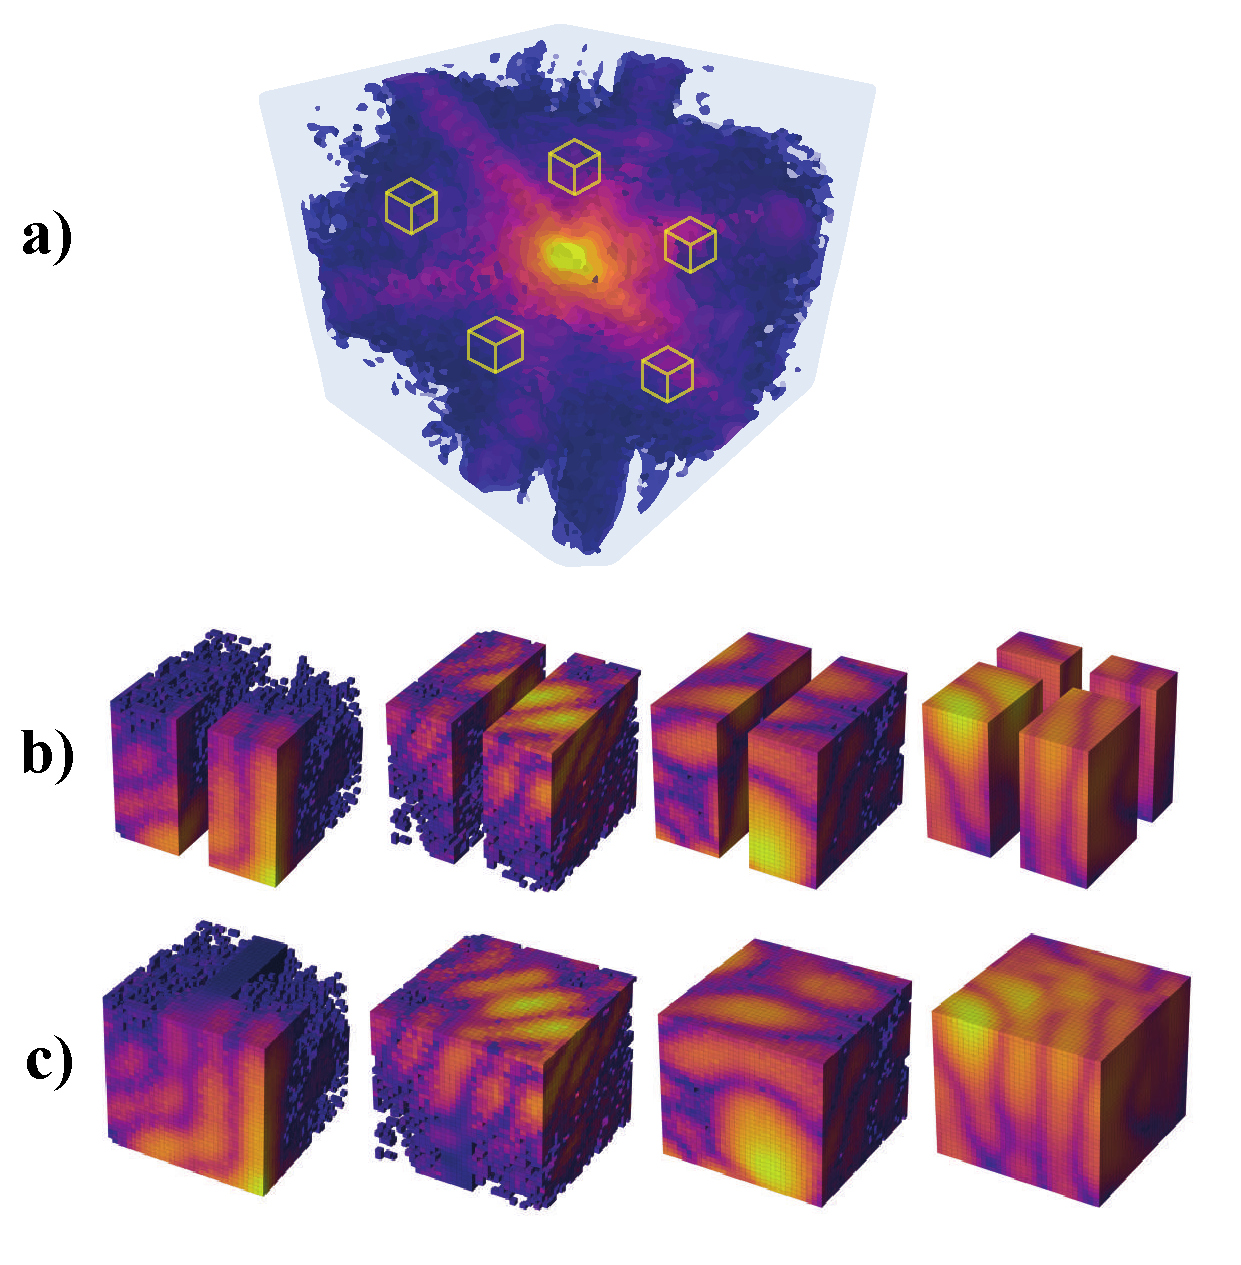
\includegraphics[width=.6\textwidth]{figures/Inpainting/process.pdf}
    \caption{\textbf{Schematic of the patches extraction.} \textbf{a)} The 3D BCDI diffraction pattern and the 
    patches. \textbf{b)} $32\times32\times32$ pixel-size patches with 9 pixel-wide vertical and cross-shaped gaps.
    \textbf{c)} Same patches with the DL inpainted gaps.}
    \label{fig:patches_method}
\end{figure}

\section{3D model architecture}

The DL architecture used for the 3D patching inpainting is illustrated in Fig. \ref{fig:architecture3d}.  
Given the reduced size of the inputs, the encoder was composed of four blocks only, in each of which there
were convolutional layers and max pooling layers. The feature map was thus reduced to a $2\times2\times2\times478$ tensor 
before being passed to the decoder. Notice that, as introduced above in section Sec.\ref{sec:model},
dilated convolutions were employed in the first two blocks to enhance the extraction long-range correlated features. 
After four decoder blocks three simple convolutional layers with 24,12 and 6 channels were used respectively in 
order to restore the possible smoothing effect of the decoder. As in the 2D model, the last activation function is 
a sigmoid that ensures the output to be in the range (0,1). 
The model contains 2'770'000 trainable parameters, significantly less than the 2D models working on full size patterns. 
\\
The training was performed loading batches of 32 images at the time over 100 epochs using ADAM optimizer \cite{ADAM}. 
The optimizer was initialized with a learning rate of $10^{-3}$ and decreased it progressively with the 
\texttt{ReduceLROn-Plateau} callback feature available in Tensorflow. In order to exploit the maximum of the training 
dataset only 4\% and 2.5\% of the whole dataset was left for validation and testing respectively.  

\begin{figure}[h]
    \centering
    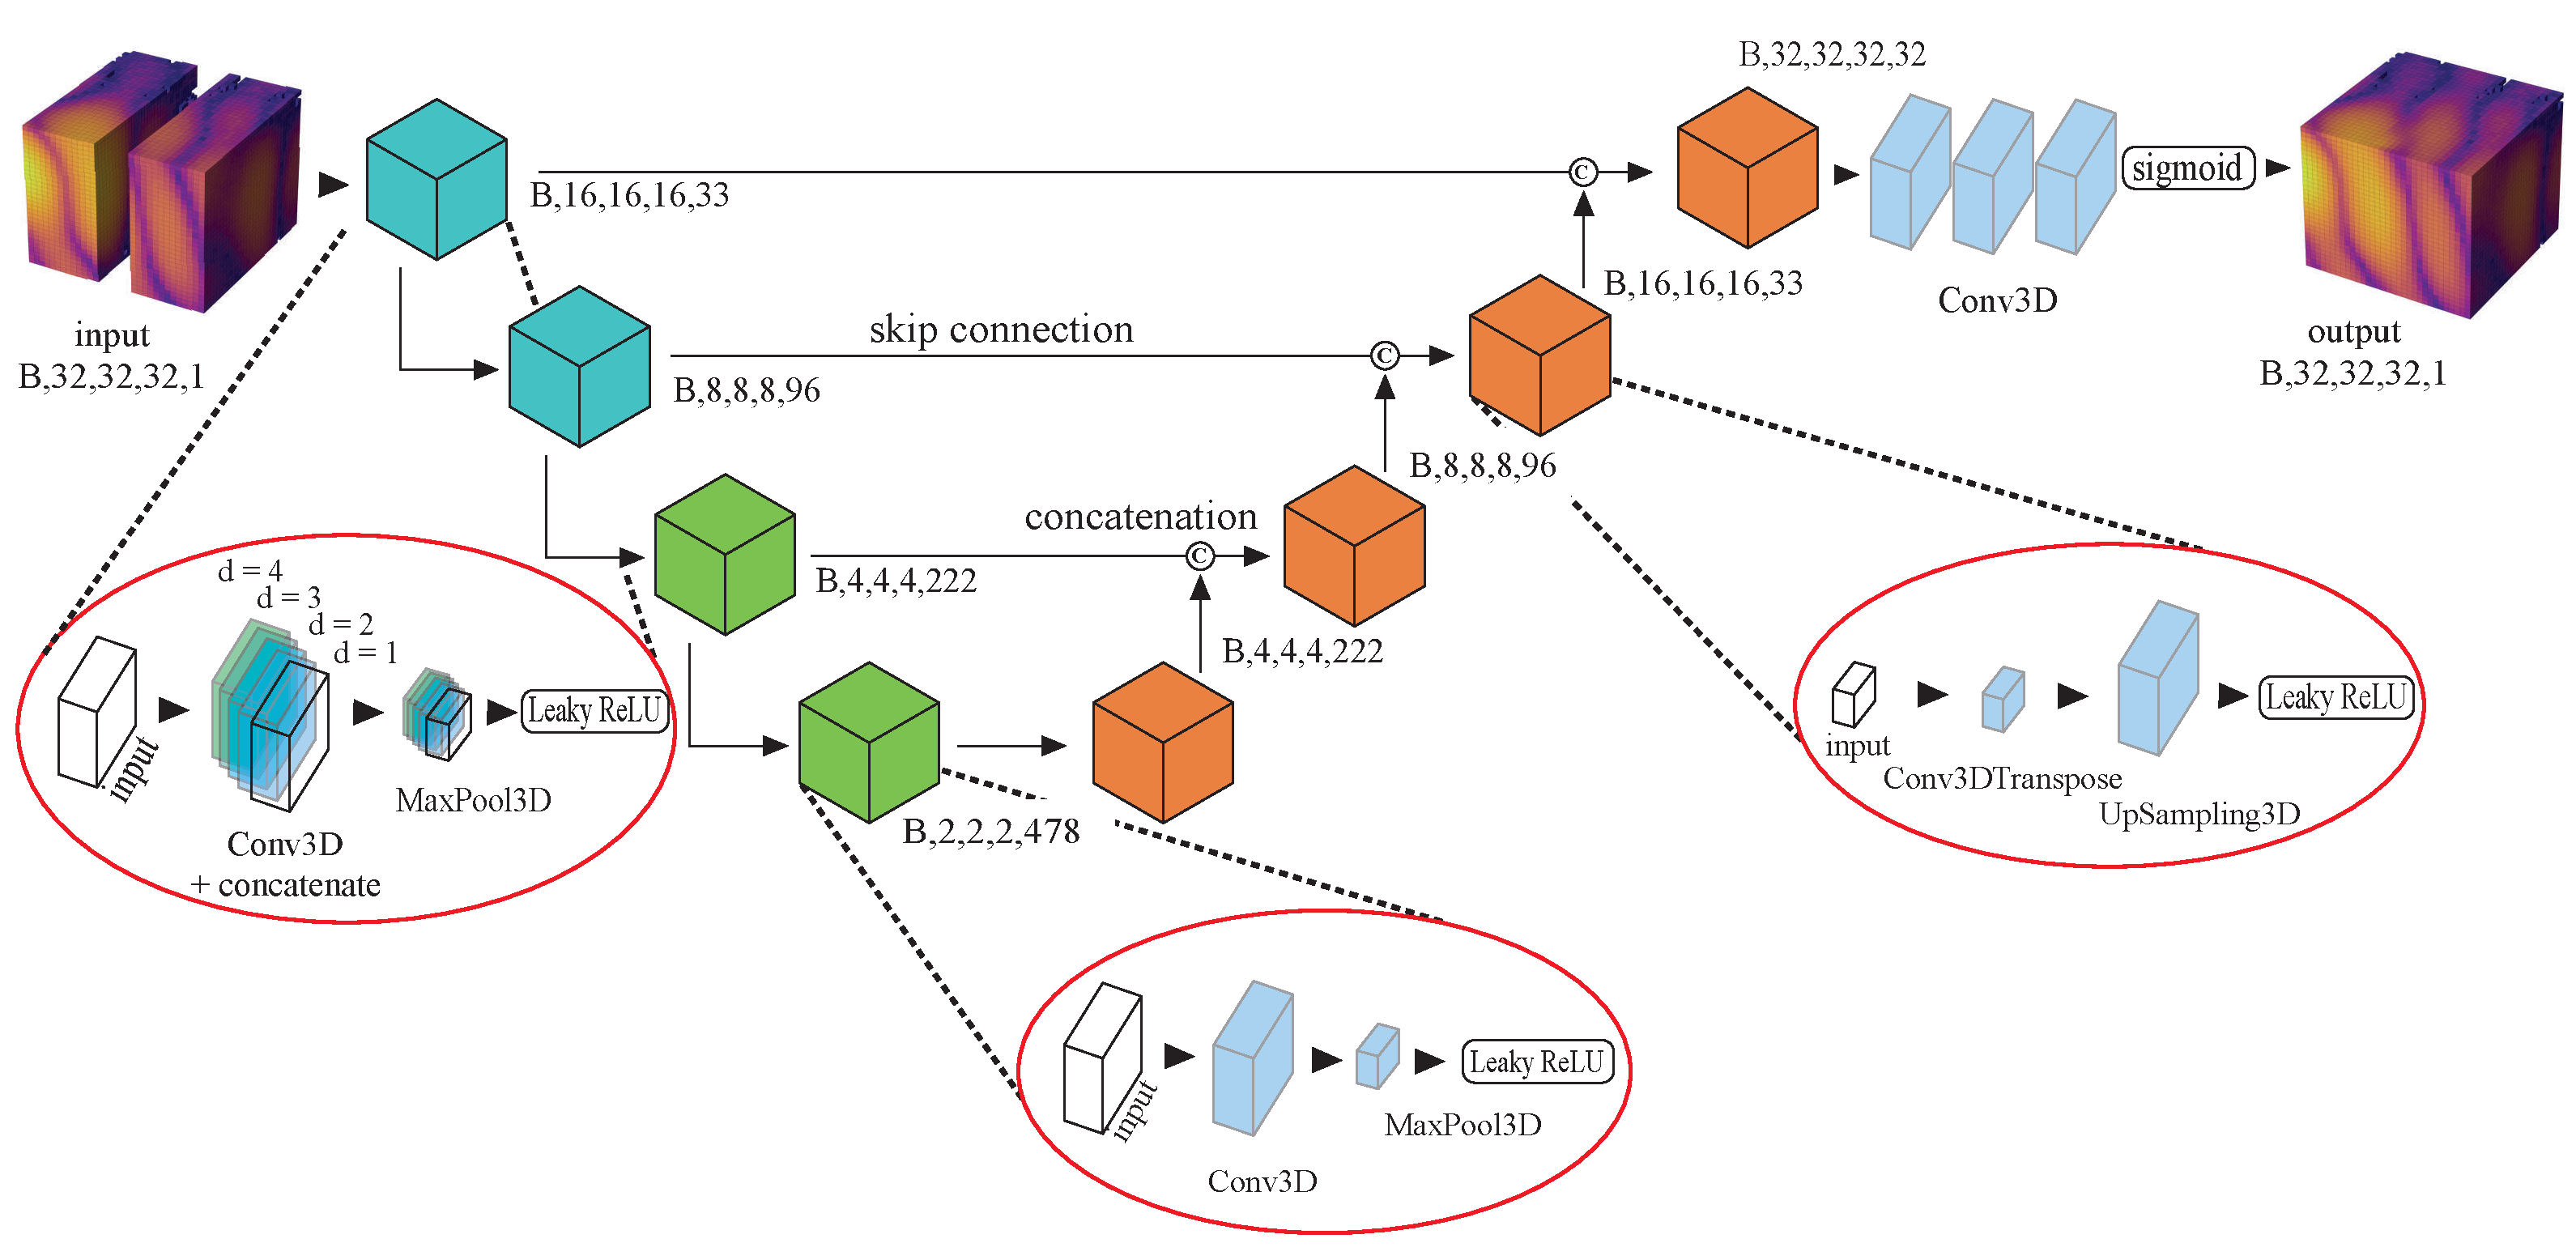
\includegraphics[width=\textwidth]{figures/Inpainting/Architecture_compressed.pdf}
    \caption{\textbf{Schematic of the 3D model architecture} The model uses a modified U-Net structure. 
    In the first two encoder blocks (highlighted by the left red circle), dilated convolutions are applied where the 
    original input is concatenated with its convolutions at various dilation rates (\textit{d = 4,3,2,1}) prior 
    to the MaxPooling operation. The input consists of small gap-affected portions, grouped into batches
     of 32 (B). These portions (top left) are progressively processed by the encoder until they are reduced to a 
     $ 2\times2\times2$ pixel-size feature map. In the decoder, each building block (represented as orange cubes) receives 
     as input the concatenation of the output from the previous block and the matching output from the encoder block 
     of the same size. The final result (top right) is a batch of inpainted versions of the input portions.}

    \label{fig:architecture3d}
\end{figure}

\section{Results in detector space}\label{sec:res_rec}

In this section the results of the DL model on both simulated and experimental diffraction patterns are presented. 
The following section will focus on the results in real space and the reduction of the artifacts 
in the reconstructed objects.\\

Once completed the training, the model was first tested on portions taken from the test dataset. It is possible
to qualitatively observe that the model works equally well for both simulated and experimental data (see Figs. \ref{fig:pred_portions_sim}
- \ref{fig:pred_portions_exp}). From a first visual assessment one can also confirm that low noise regions with larger features
are better restored than others as previously stated in Sec. \ref{sec:performances}. Another curious effect that can observed, 
is the ``smoothening'' of features around noisy areas (see first column in Fig. \ref{fig:pred_portions_sim} and last column in Fig.
- \ref{fig:pred_portions_exp}). In fact, the ``grainy'' aspect of these regions is caused by Poisson noise which cannot
be predicted by the DL model as it is uncorrelated. In those regions the DL performs therefore an averaging that 
``smoothens'' the features and acts like a denoiser. This effect has been already studied in the literature and exploited 
for denoising applications like the Noise2Void model \cite{Noise2Void}.

\begin{figure}[H]
    \centering
    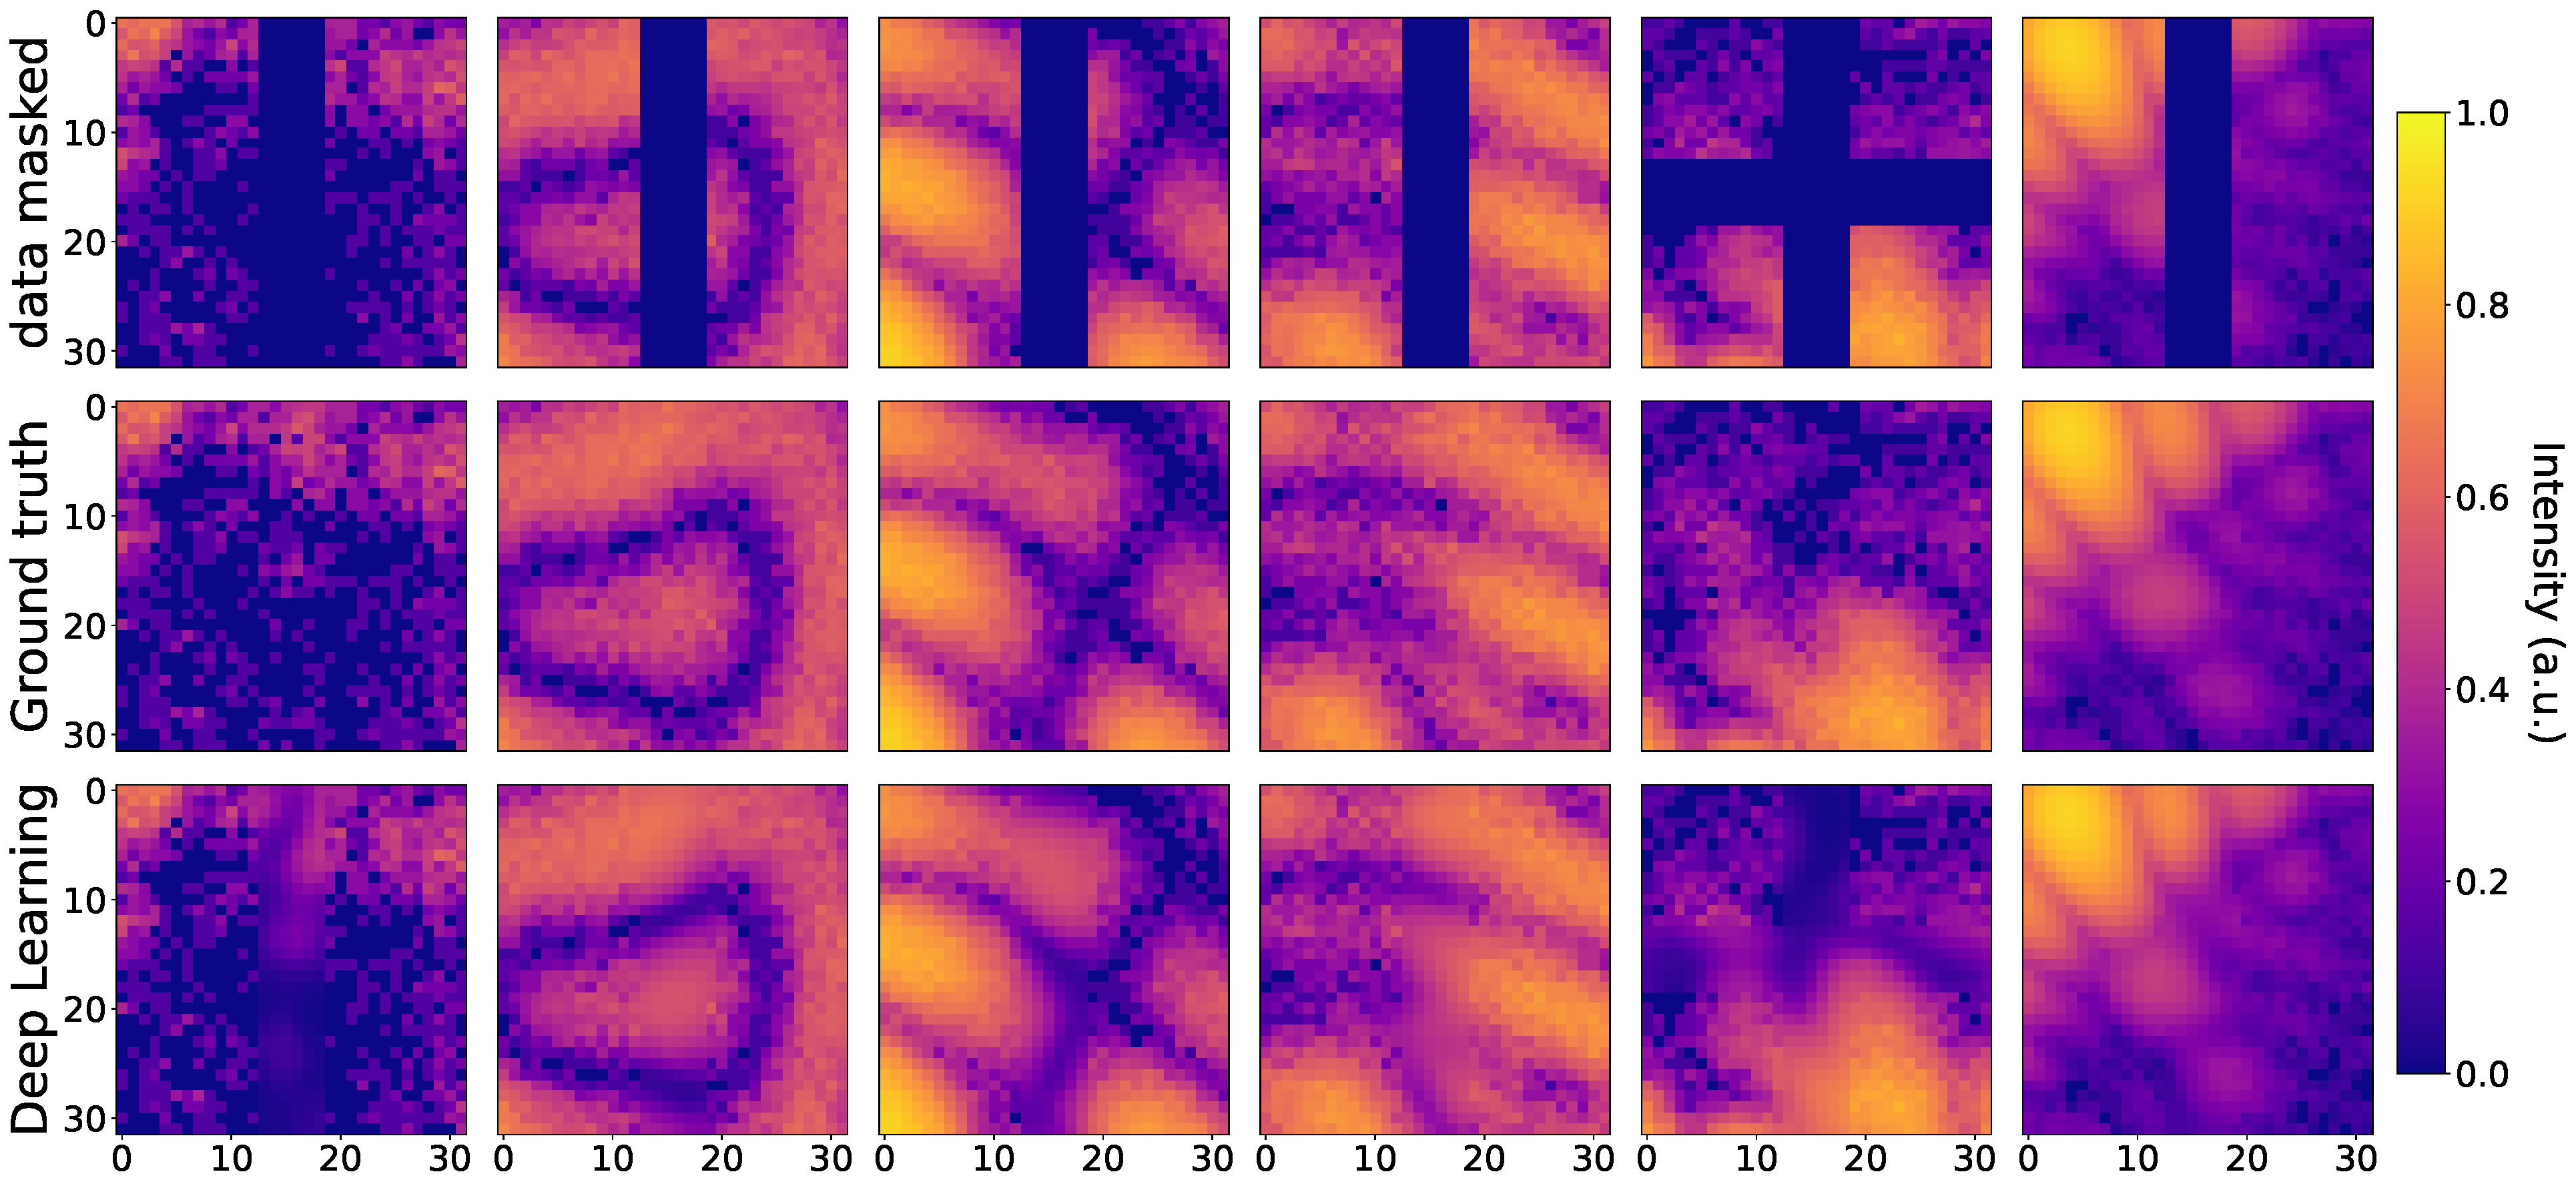
\includegraphics[width=\textwidth]{figures/Inpainting/prediction_small_simulated.pdf}
    \caption{\textbf{Results on portions of test simulated data}. Central slices of portions taken from the simulated test
    dataset. Masked input with 6 pixel-wide gap in the first row, corresponding ground truth and DL inpainted in second and third
    row respectively.}
    \label{fig:pred_portions_sim}
\end{figure}

\begin{figure}[H]
    \centering
    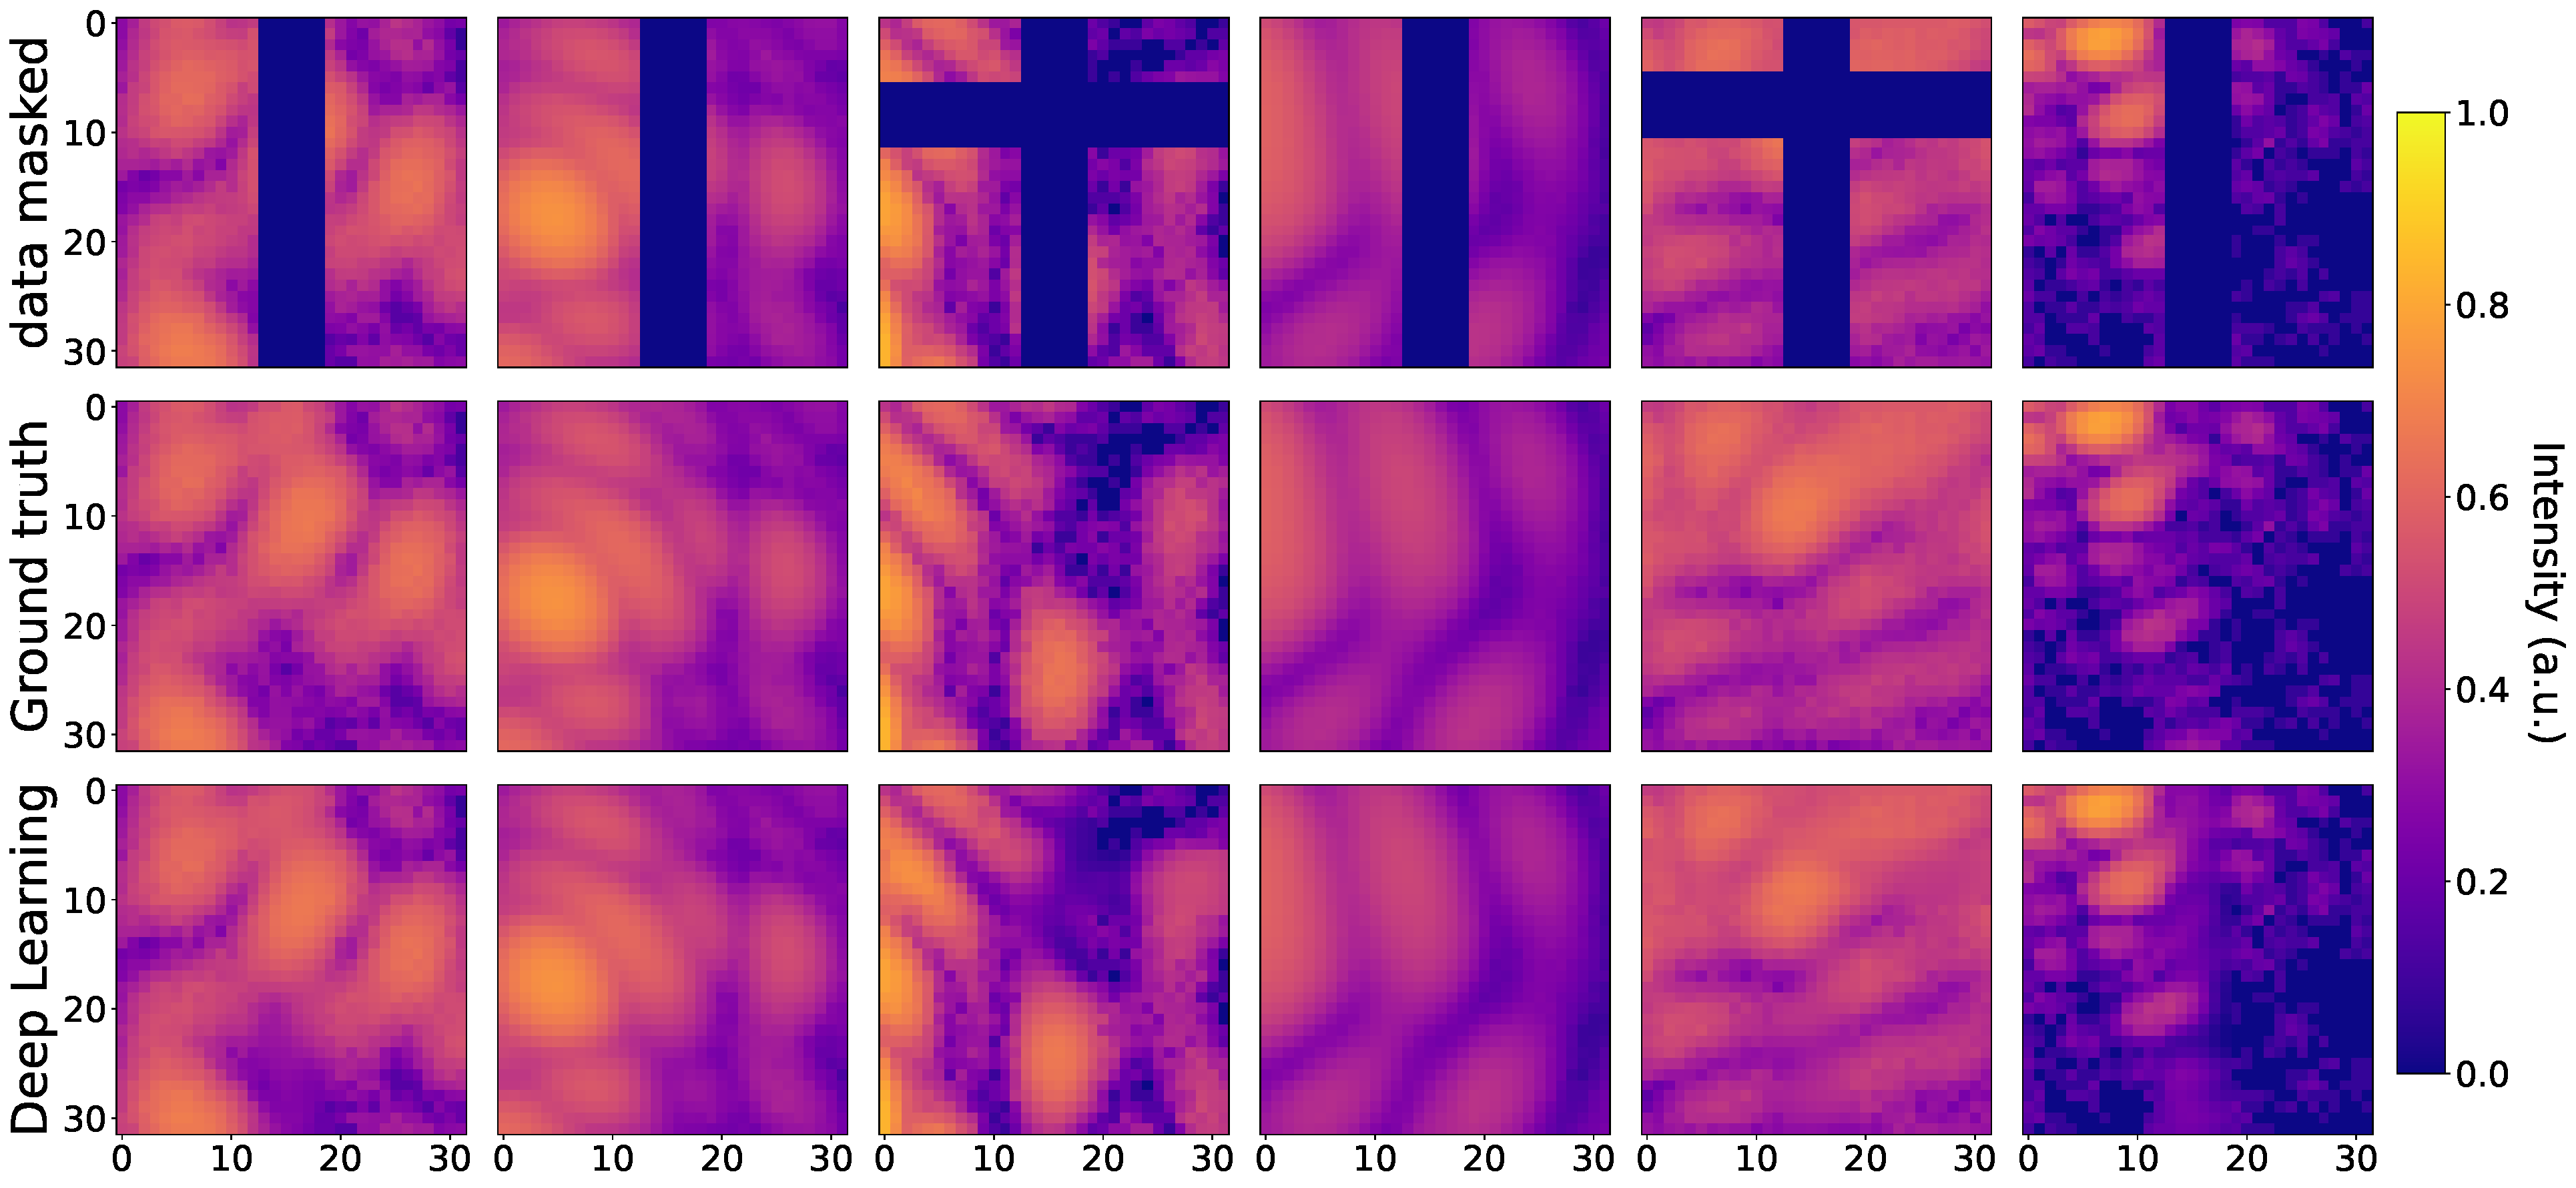
\includegraphics[width=\textwidth]{figures/Inpainting/prediction_small_experiment.pdf}
    \caption{\textbf{Results on portions of test experimental data}. Central slices of portions taken from the experimental test
    dataset. Masked input with 6 pixel-wide gap in the first row, corresponding ground truth and DL inpainted in second and third
    row respectively.}
    \label{fig:pred_portions_exp}
\end{figure}

\subsection{Full gap inpainting}\label{sec:full_gap}

For the inpainting of a gap inside a full 3D BCDI pattern it is sufficient to apply repeatedly the DL model on sub-volumes 
cropped such that the gap plane lies vertical in the center of the array perpendicularly to the third dimension. Each sub-
volume needs to be preprocessed exactly in the same way described above, i.e. transformed into logarithmic scale and 
normalized between 0 and 1. Moreover, it is advised to apply a mask on the gap, to match exactly the gap width the model
has been trained with. 
One can then proceed along the gap moving forward one pixel at the time, compute the inpainted gap and average the prediction
over the overlapping pixels with the previous predictions. By doing this, potential errors are averaged out and the accuracy
of the prediction is maximized. However, for large datasets this can be time-consuming. For example, for a $128\times128\times128$ pixel-size
diffraction pattern with a cross-shaped gap the time needed to compute the full inpainting amounts to 11 minutes (using a 
NVIDIA Tesla V100-SXM2 GPU with 32GB RAM). However, it is possible to increase the step size to significantly reduce the computing
time without affecting excessively the accuracy (see Fig.\ref{fig:skip_figure}). It was proven that the amount of time for the full inpainting follows a power 
law (see Fig. \ref{fig:skip_case}a) and the accuracy starts dropping significantly for more than 5 pixels skipped at the time
(see Fig. \ref{fig:skip_case}b).  

\begin{figure}[H]
    \centering
    \begin{subfigure}{0.45\textwidth} % Adjust width as needed
        \centering
        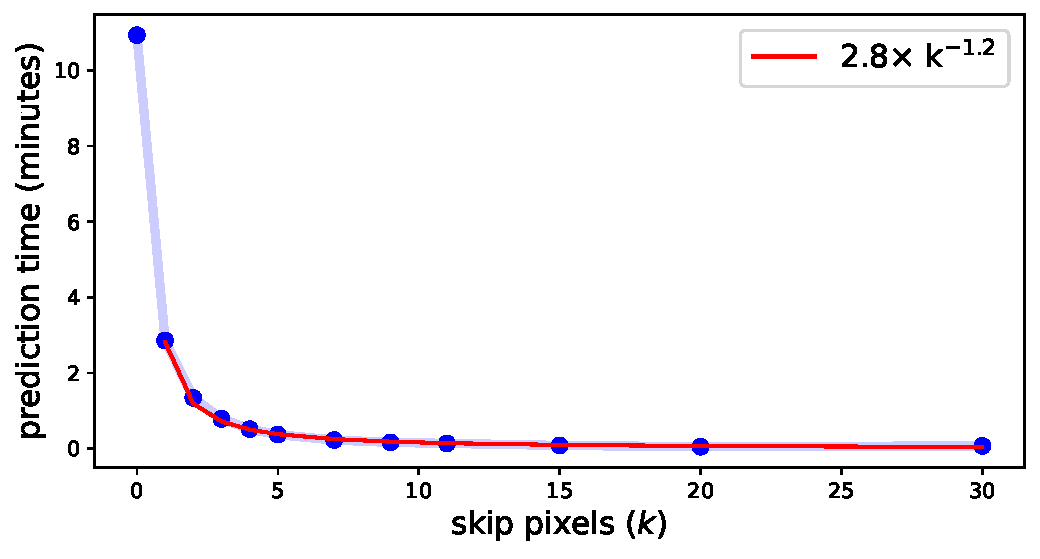
\includegraphics[width=\linewidth]{figures/Inpainting/skip_pixels_time.pdf}
        \caption*{}
    \end{subfigure}
    \hfill
    \begin{subfigure}{0.45\textwidth}
        \centering
        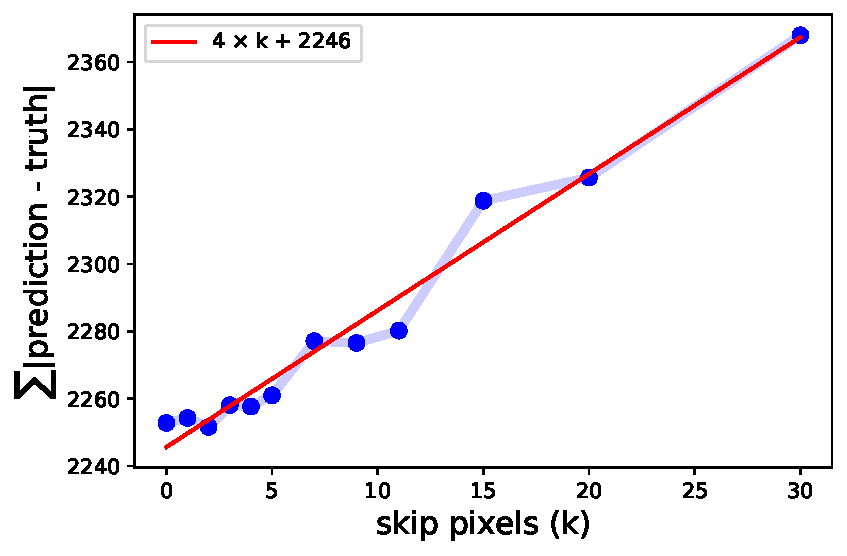
\includegraphics[width=\linewidth]{figures/Inpainting/skip_error.pdf}
        \caption*{}
    \end{subfigure}
    \caption{\textbf{Left} Full inpainting time for a 6 pixel-wide cross-shaped gap on a  $128\times128\times128$ pixel-size
    diffraction pattern as function of the step size, i.e. the amount of pixels skipped between patch DL predictions along the gap.
    \textbf{Right} Sum of the absolute errors as function of the skipped pixels. }
    \label{fig:skip_case}
\end{figure}

\begin{figure}[H]
    \centering
    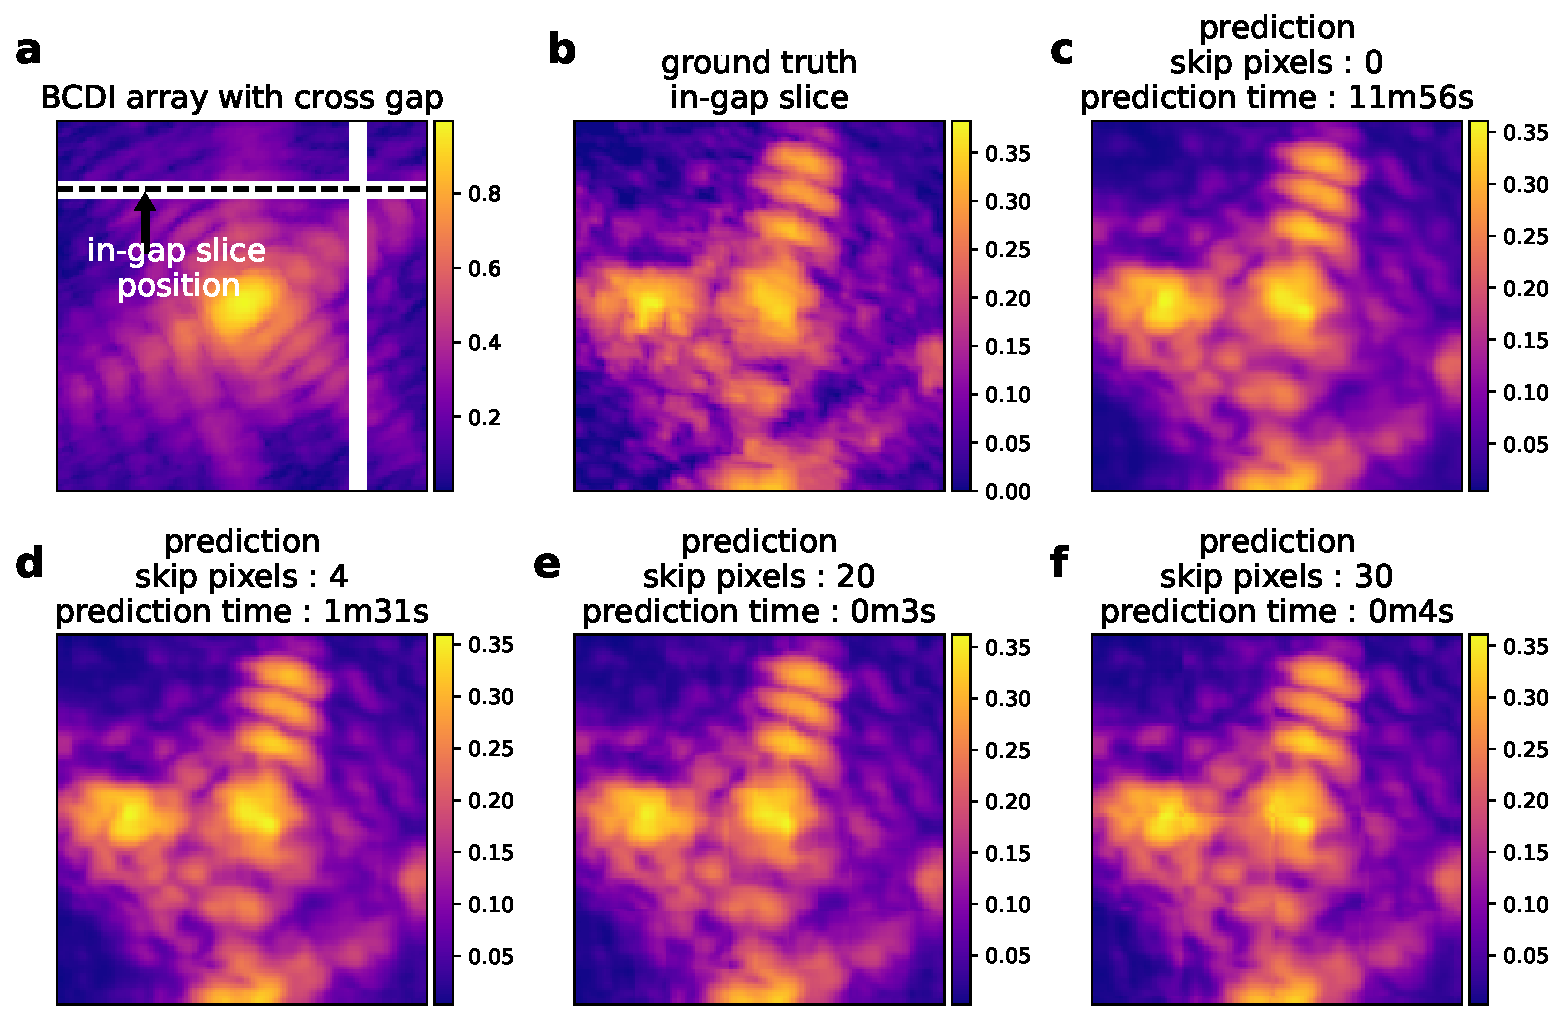
\includegraphics[width=\textwidth]{figures/Inpainting/Skip_pixels_ingap_slice.pdf}
    \caption{Full inpainting of an experimental BCDI pattern for different amounts of skipped pixels. \textbf{a}
    slice of the diffraction pattern perpendicular to the gap plane.\textbf{b} Ground truth intensity inside the gap.
    \textbf{c-d-e-f} In-gap prediction with 0, 4, 20 and 30 skipped pixels respectively, with corresponding 
    execution time. Skipping 4 pixels is a good trade off between time and accuracy.}
    \label{fig:skip_figure}
\end{figure}

\newpage

\section{Performance assessment}\label{sec:performances}

In order to assess the DL model's performance with respect to other inpainting methods, it was tested against 
conventional interpolation methods. Specifically, an experimental BCDI pattern with a 6 pixel-wide 
cross-shaped gap was considered and the inpainting results of the DL model with (i) linear interpolation (ii) cubic interpolation 
(iii) nearest-neighbor interpolation were compared. These techniques allow for a quick estimation of the intensity distribution 
inside the gaps but fail to recover fine features (see Figs. \ref{fig:interp}). In particular, it can be noticed 
in the \textit{in-gap slice} (Fig. \ref{fig:interp}a) that linear interpolation for instance doesn't retrieve correctly 
the space curvature of the fringes while nearest neighbor and cubic interpolations show artifacts in correspondence 
of the perpendicular gap. When considering the central slice perpendicular to the gap planes (along the rocking curve
dimension) one can notice even more how the DL model outperforms conventional interpolations (Fig. \ref{fig:interp}b).
 

% \begin{figure}[H]
%     \centering
%     \begin{subfigure}{0.52\textwidth} 
%         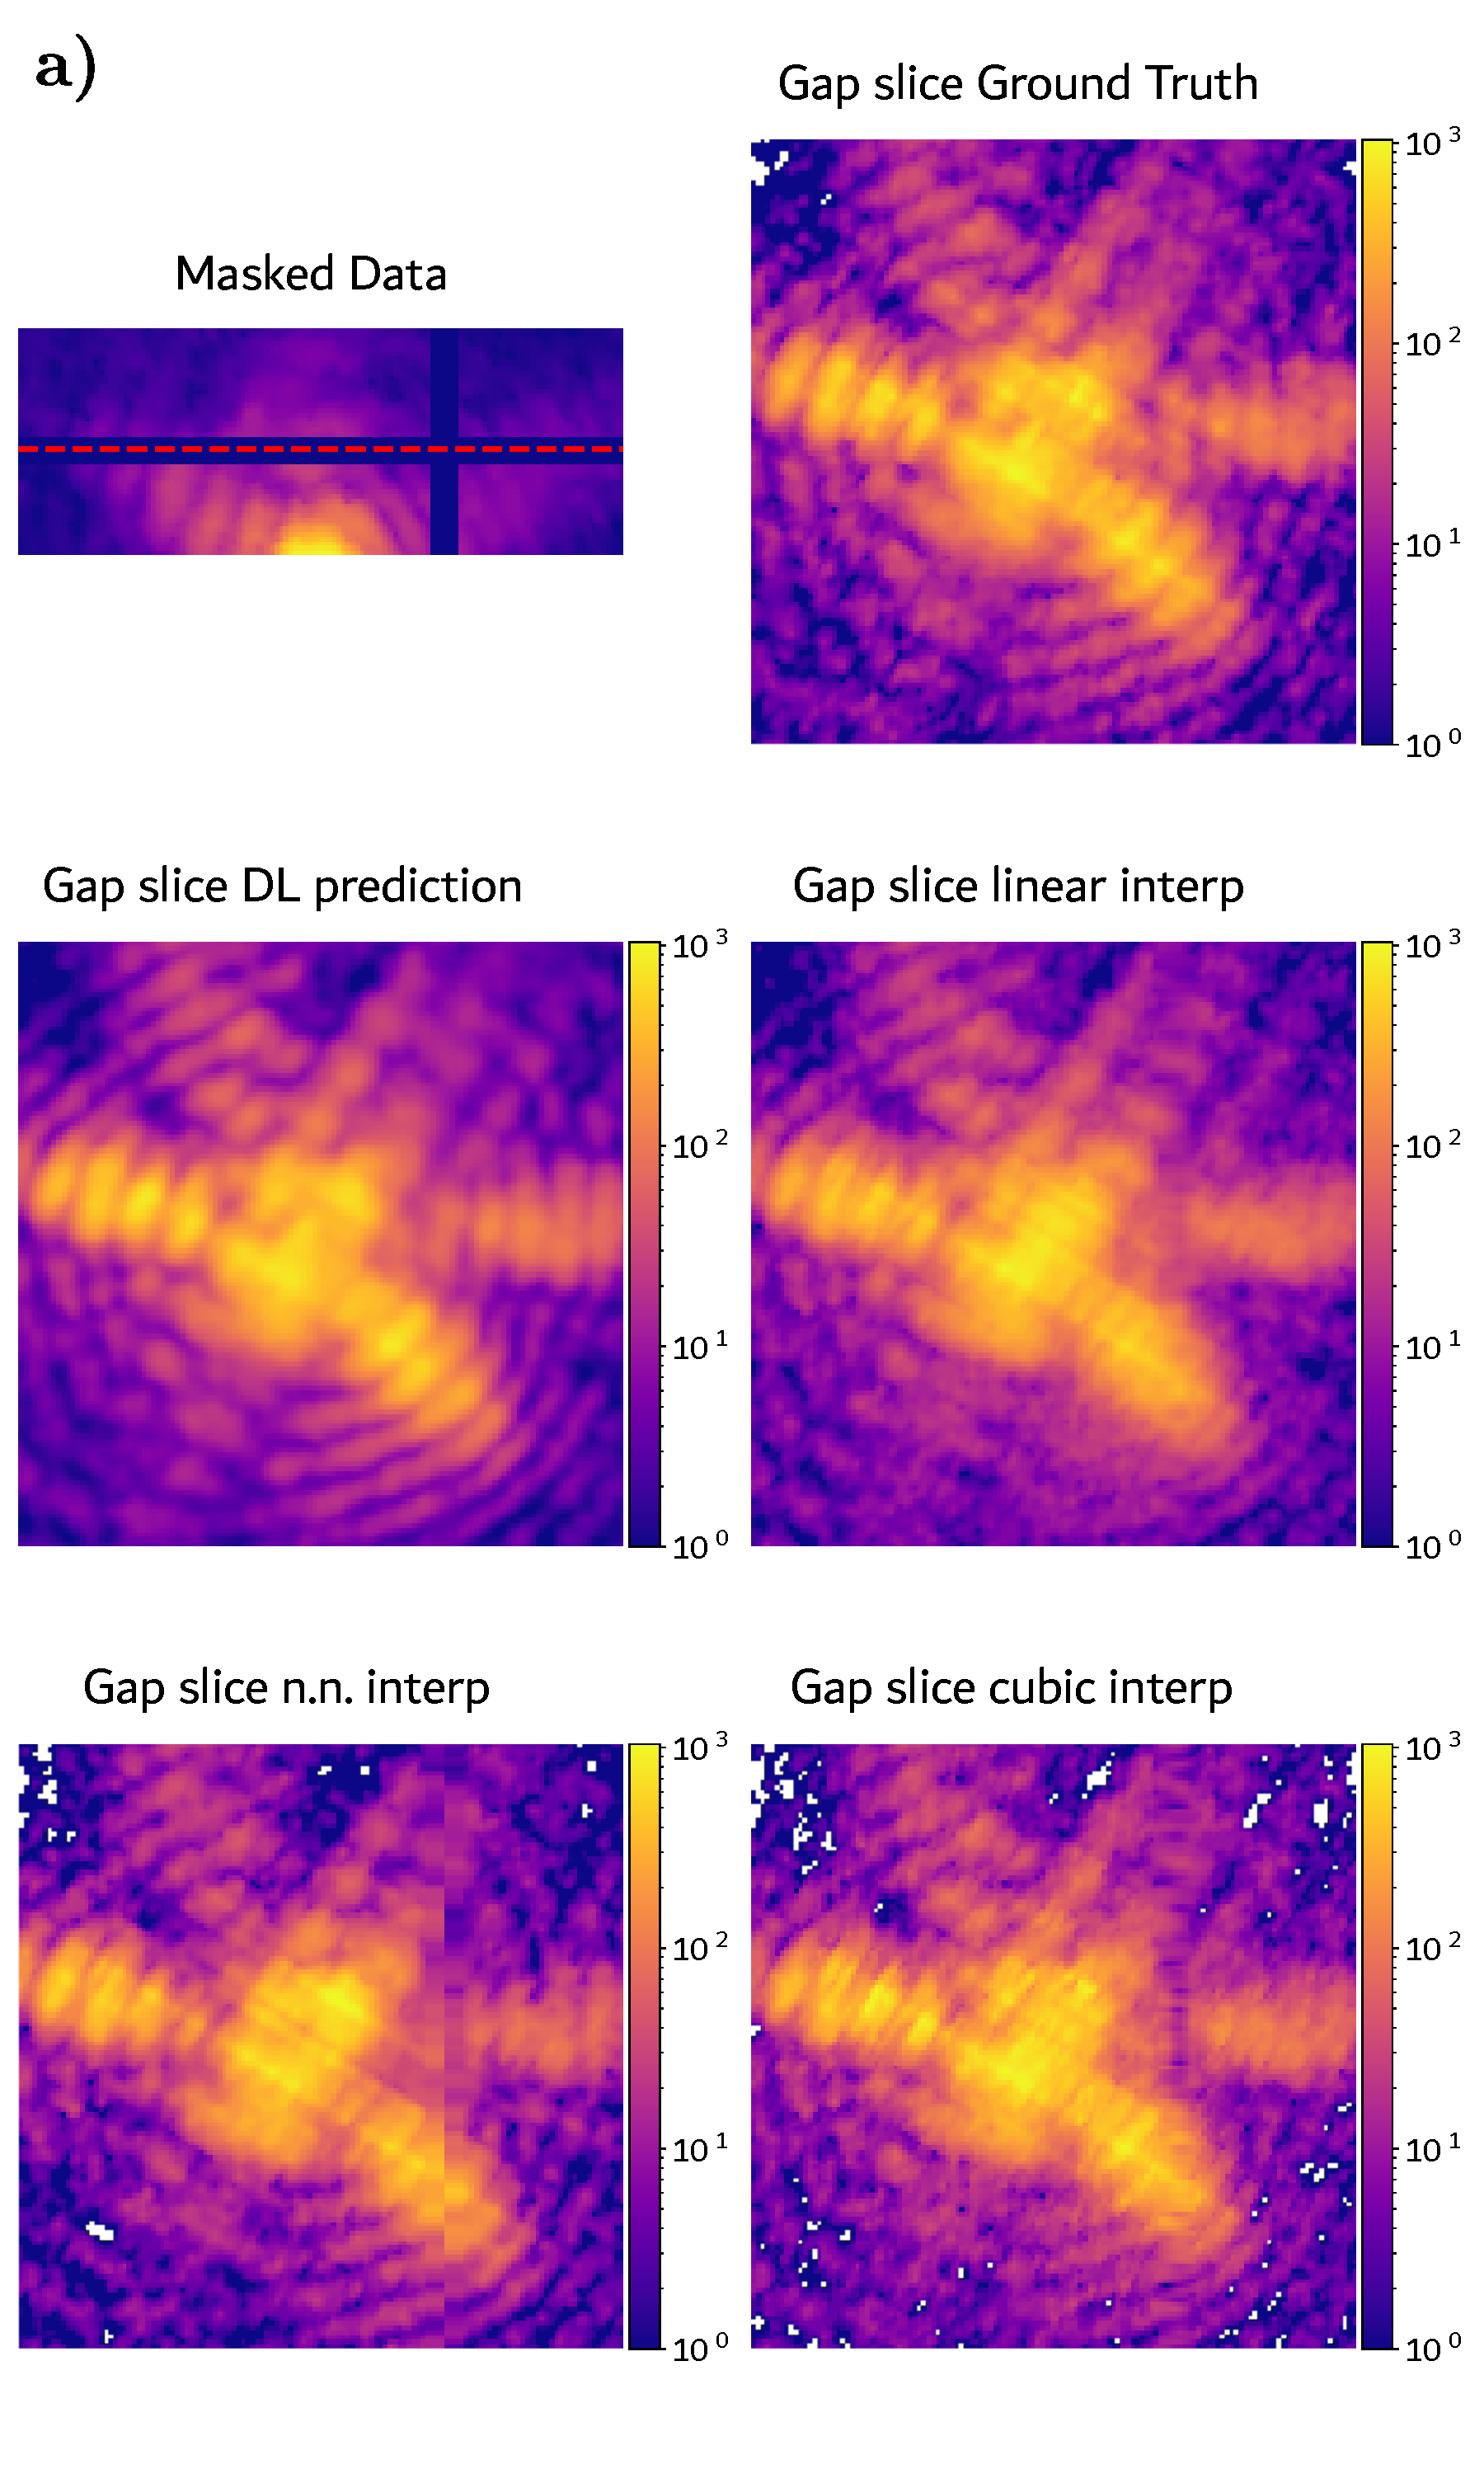
\includegraphics[width=\linewidth]{figures/Inpainting/newfig3_suppl.pdf}
%         \caption{\textbf{(a)}}
%     \end{subfigure}
%     \hfill
%     \begin{subfigure}{0.48\textwidth}
%         \centering
%         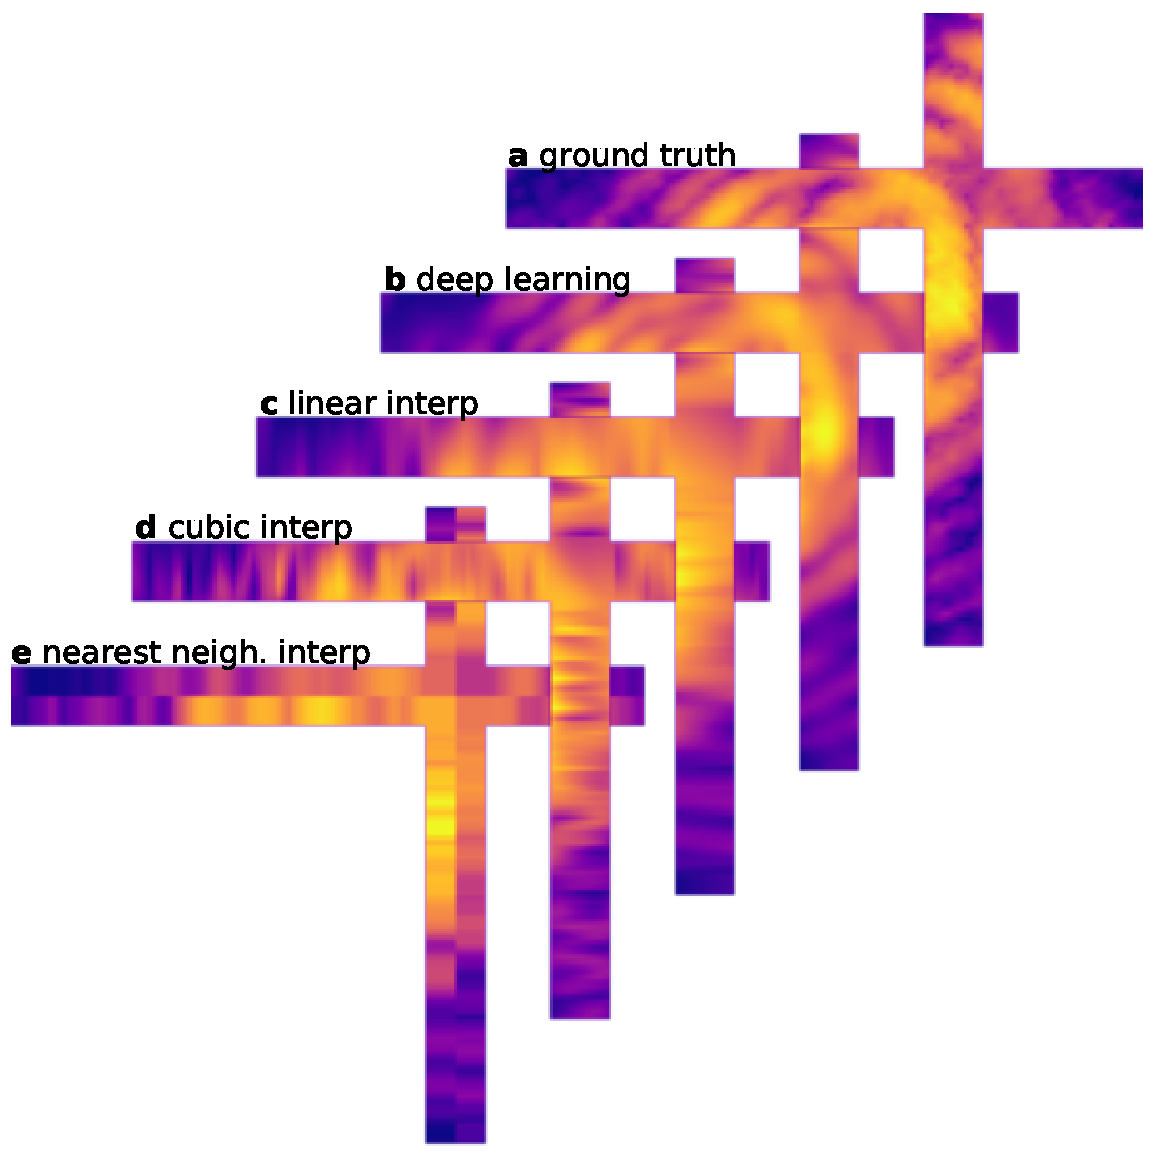
\includegraphics[width=\linewidth]{figures/Inpainting/cross_interp.pdf}
%         \caption{\textbf{(b)}}
%     \end{subfigure}
%     \caption{ }
%     \label{fig:interp}
% \end{figure}

\begin{figure}[H]
    \centering
    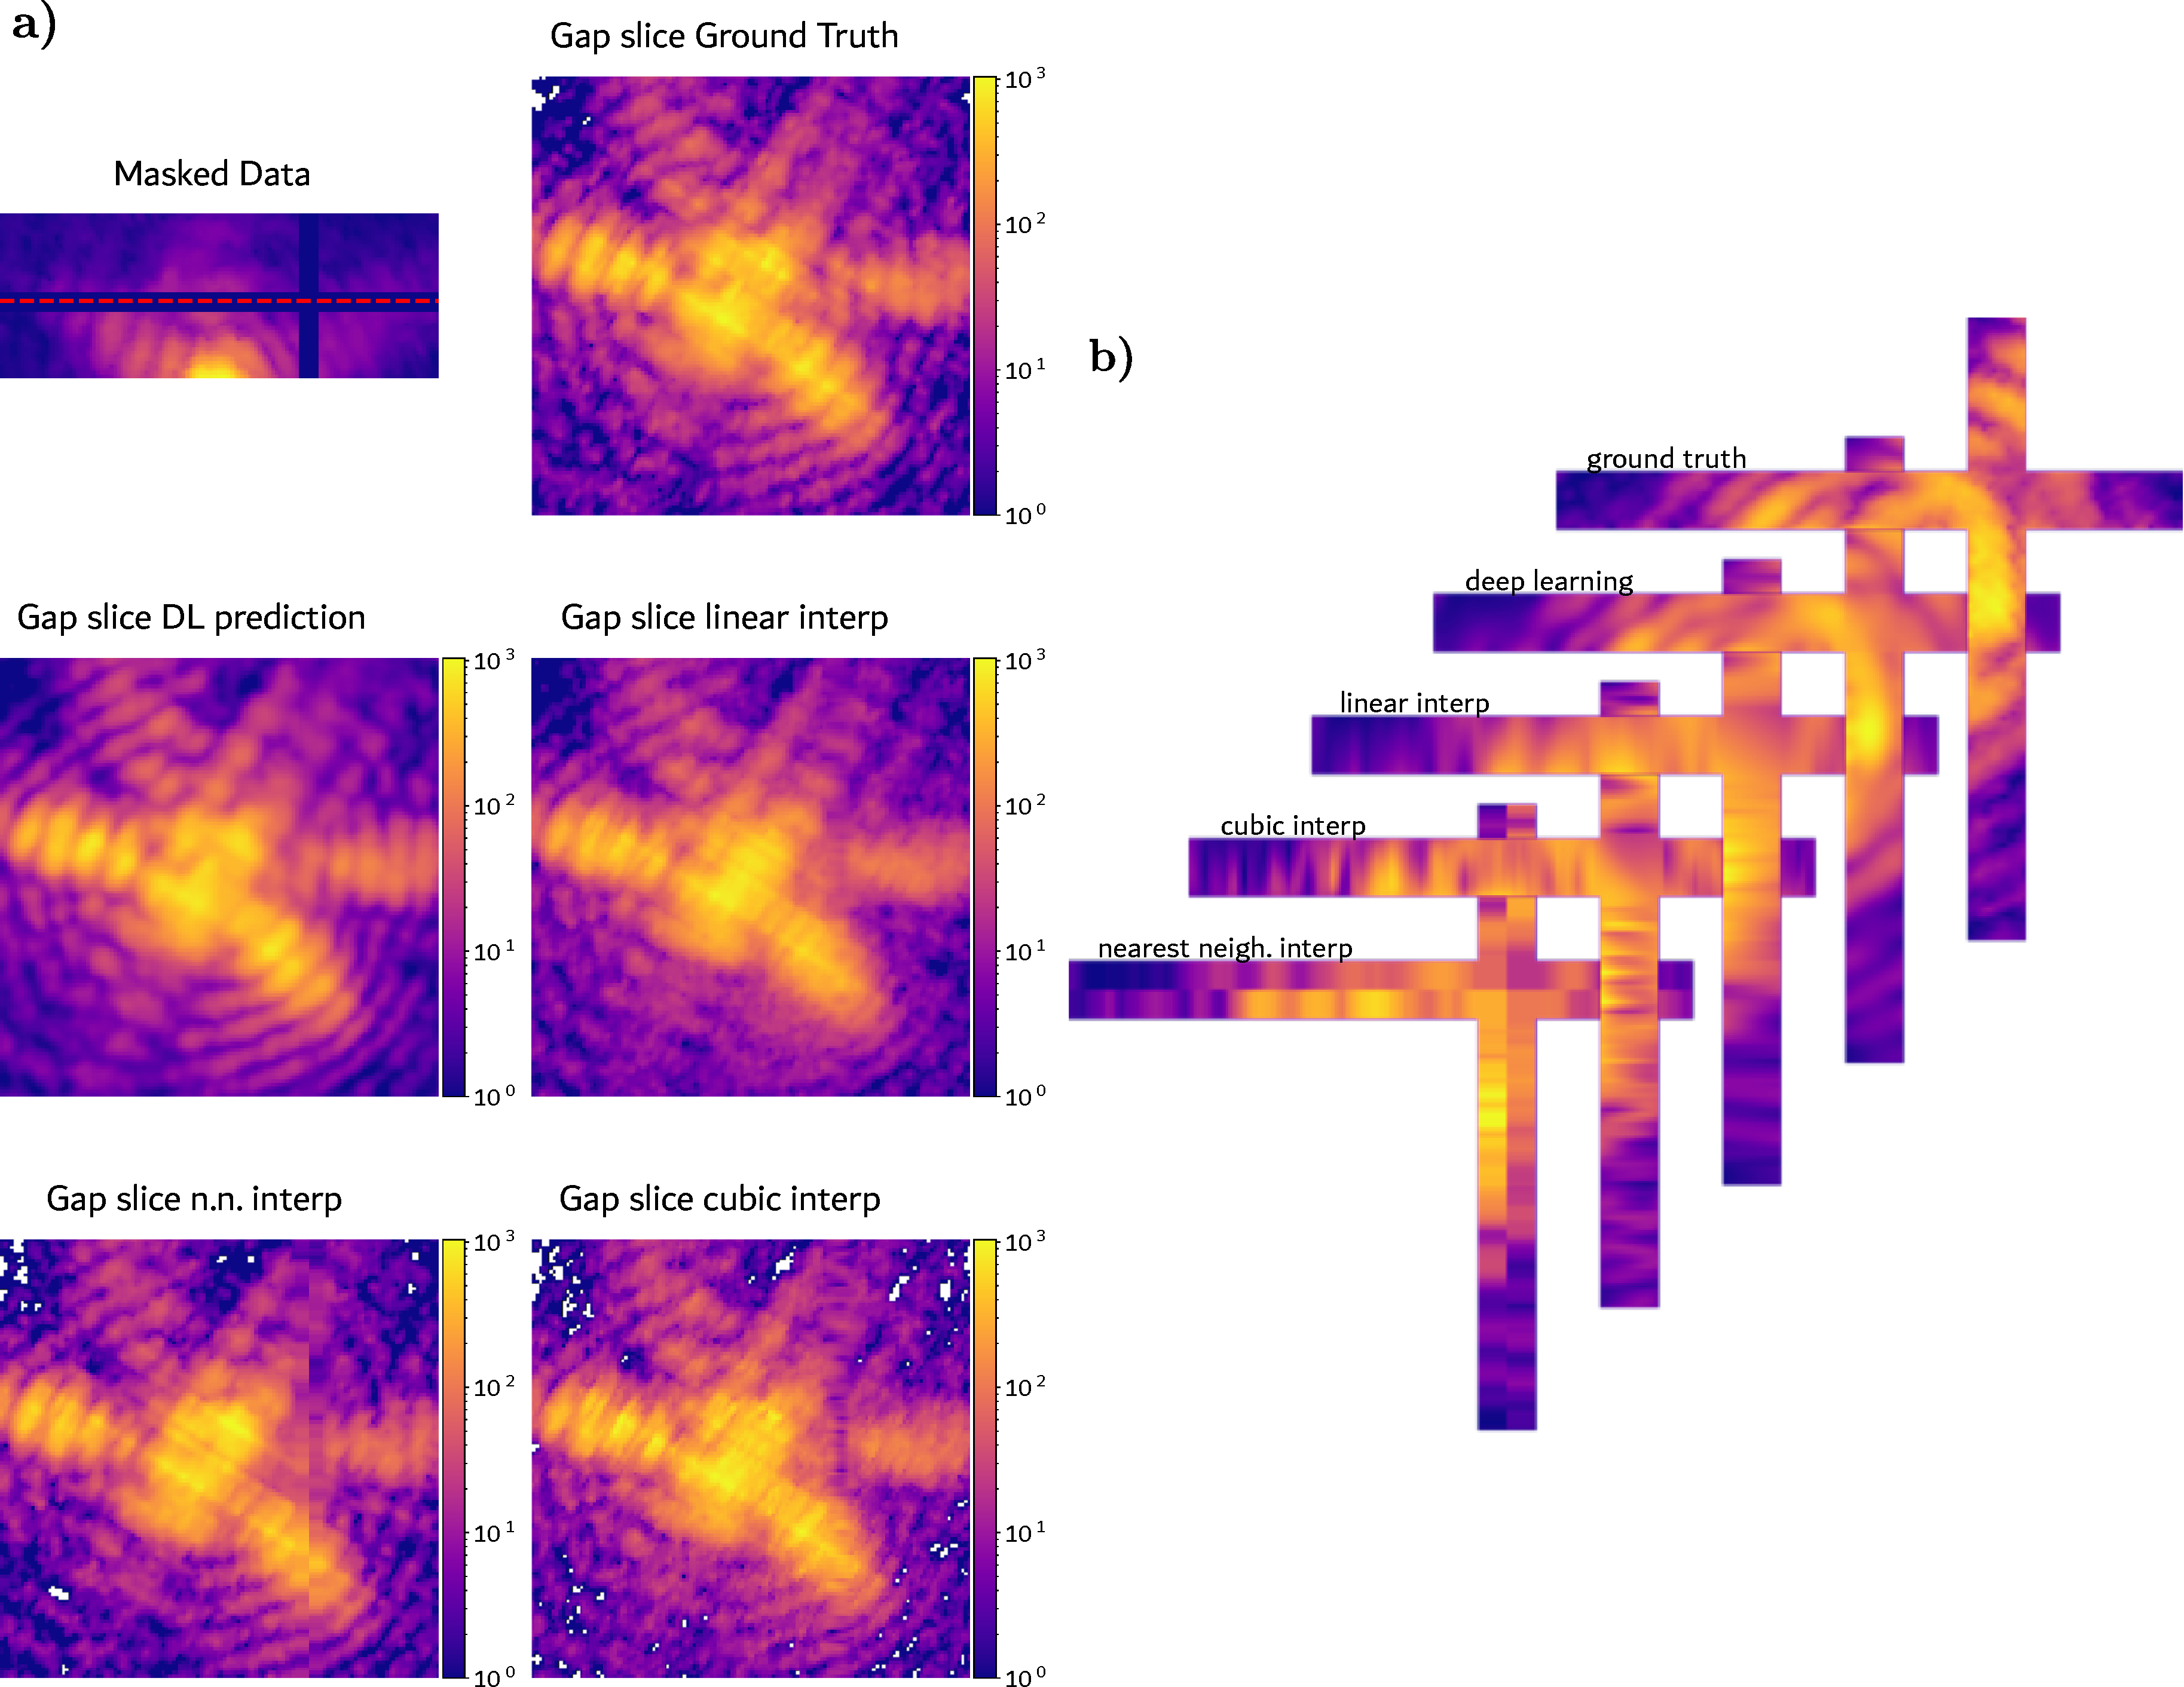
\includegraphics[width=\textwidth]{figures/Inpainting/inslice_cross_interp.pdf}
    \caption{ \textbf{Comparison of DL inpainting and standard interpolations on experimental data:} \textbf{a)} In-slice 
    cut of the ground truth data and the predictions for each inpainting method. The DL outperforms standard interpolations, 
    correctly recovering the fringes. The ``blur'' effect on the DL predicted slice is the result of the averaging of features 
    in presence of noise, typical of CNNs \cite{Noise2Void}. \textbf{b)} Cross-shaped gaps for the same dataset (perpendicular 
    view with respect to \textbf{a)}). The DL model outperforms other methods from this perspective as well. }
    \label{fig:interp}
\end{figure}

\newpage 

Similarly to the 2D case above, the performance of the model has been evaluated against the amount of intensity 
inside the sub-volume and against the oversampling ratio. The test was repeated for different gap widths, namely 3,6,9,12 
pixel-wide, using vertical gaps placed in the center of each patch. 
For the first performance assessment a full simulated $128\times128\times128$ pixel-size BCDI pattern was considered, 
and 1000 patches were randomly cropped out of it. A vertical gap was then applied in the center of each patch for different 
gap sizes and then computed the prediction with the corresponding DL model. The intensity (in photon counts) inside each patch 
was then summed and the obtained values for the 1000 samples were binned into 20 classes for better visualization. 
The accuracy scores, calculated with the PCC, were then averaged inside each bin class. The results are displayed in Fig. 
\ref{fig:acc_int_3D}. As expected from the 2D case, better accuracy scores are obtained for portions
containing larger amount of signals, where noise levels are lower and the features of the diffraction pattern are more 
visible. Moreover, the plot logically shows that smaller gaps are generally better recovered, but it is worth noticing
that the accuracy spread across different gap sizes widens for noisy portions and narrows down as the amount of signal 
increases. These trends suggest that DL models are overall robust to different gap sizes especially for high intensity regions, 
which are the most important ones as they contribute the most during the reconstruction. 

\begin{figure}[H]
    \centering
    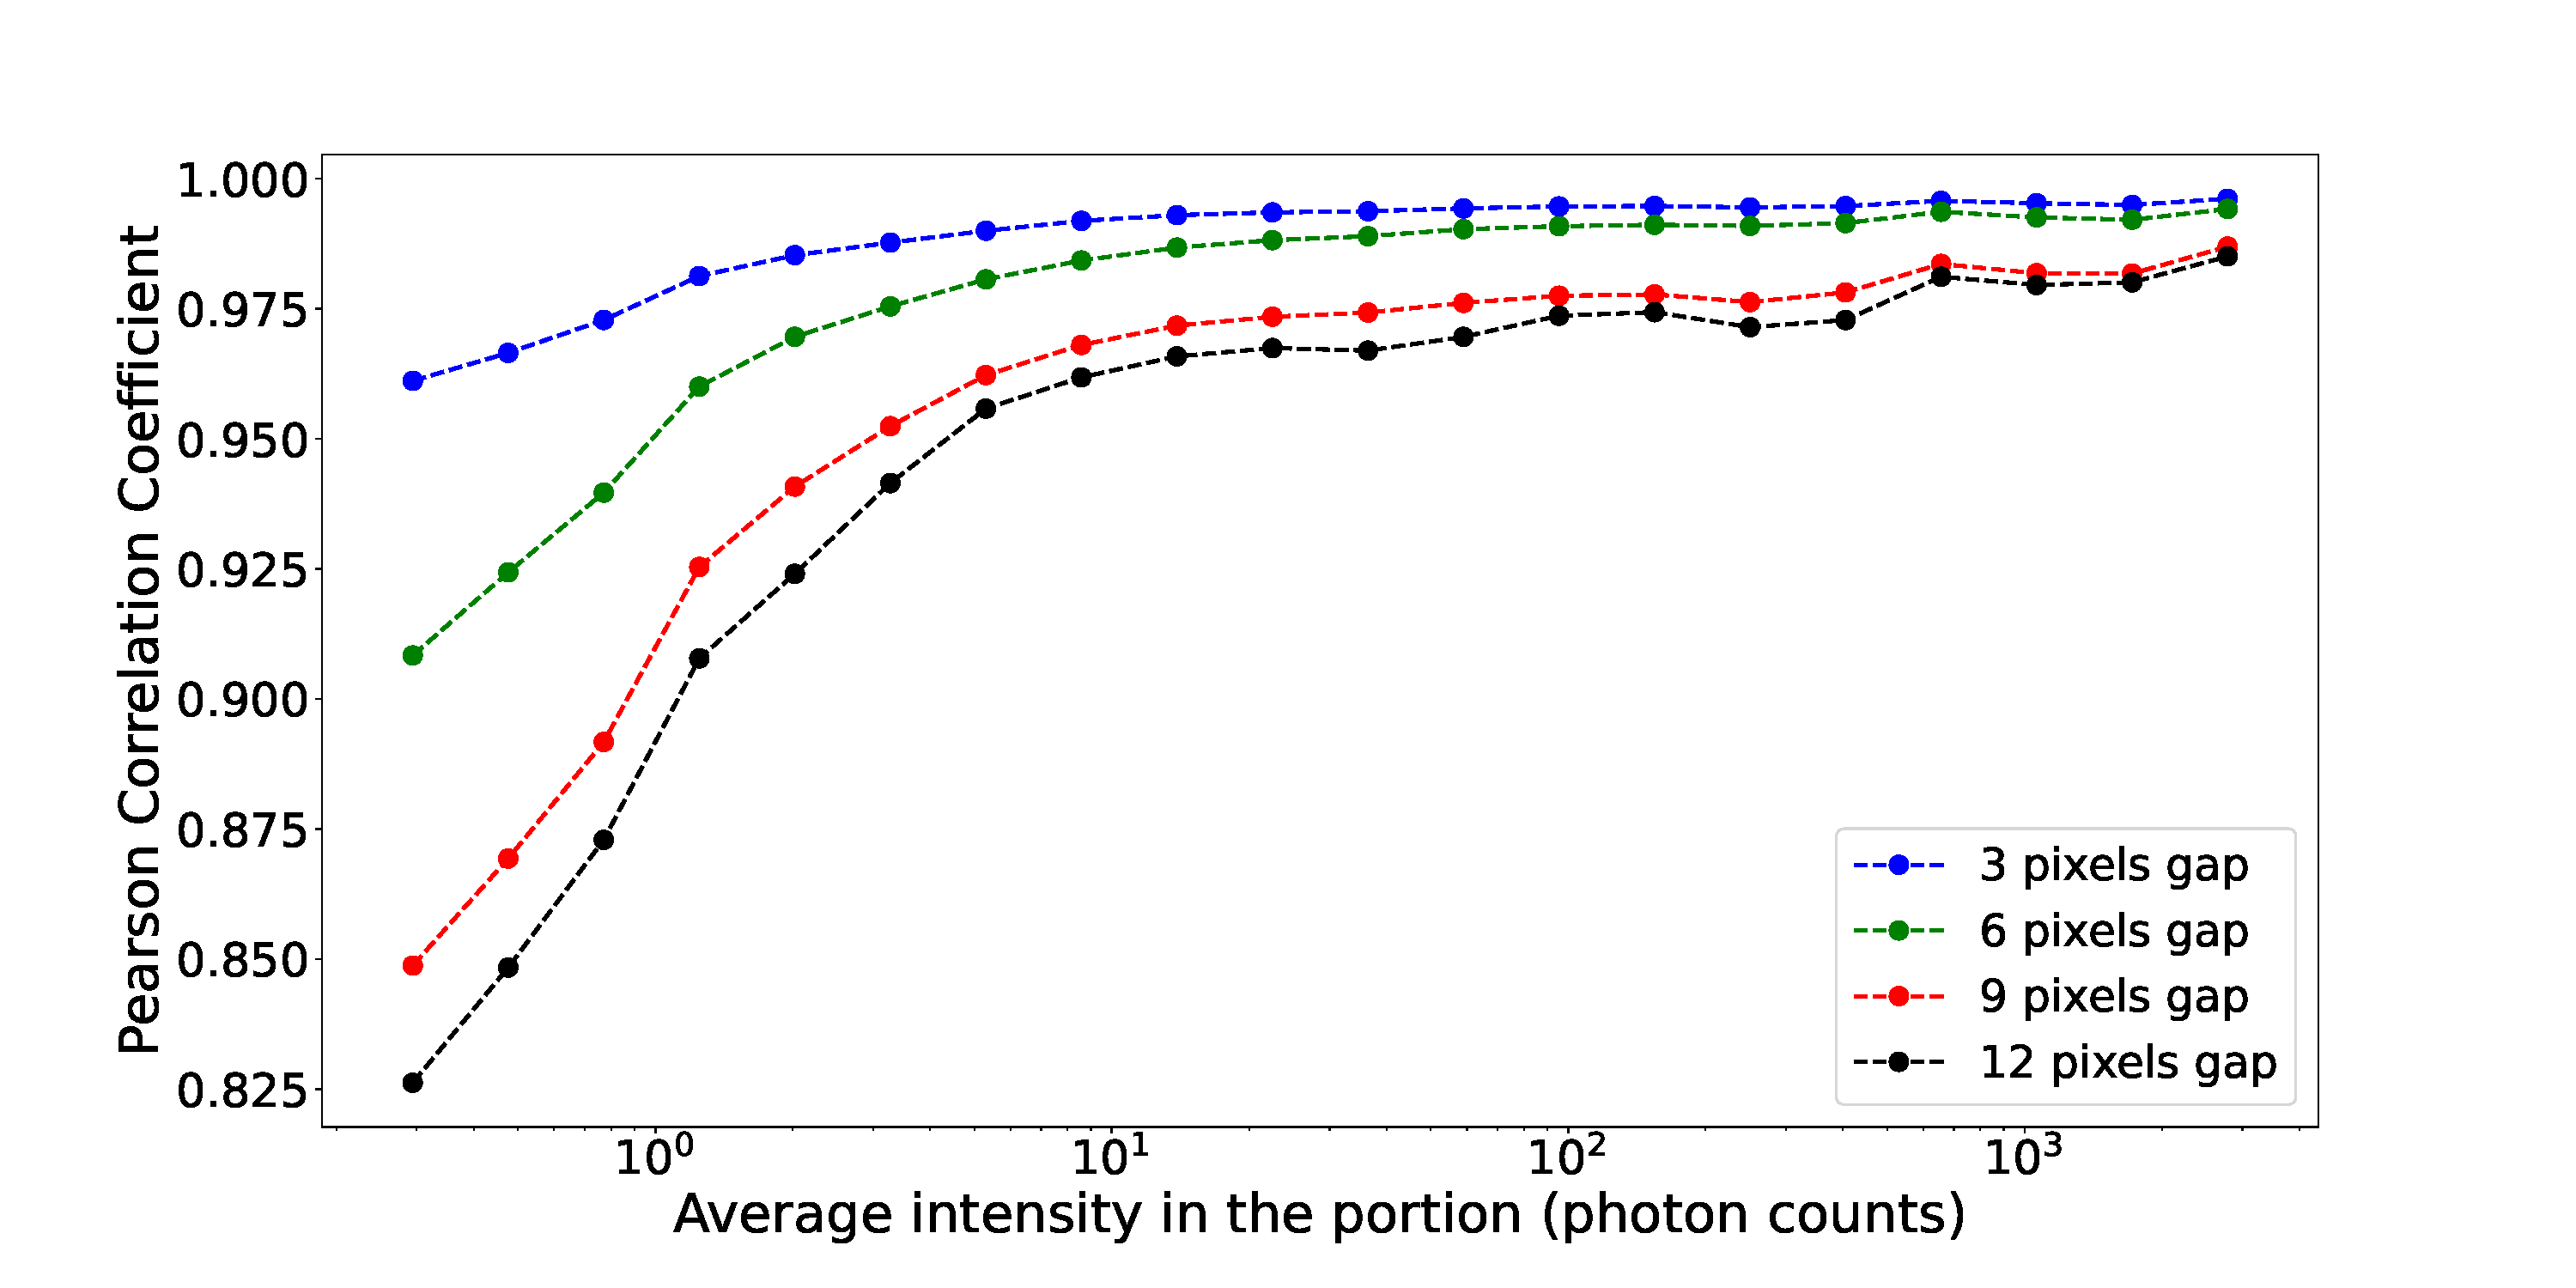
\includegraphics[width=\textwidth]{figures/Inpainting/1D_Acc_Intensity.pdf}
    \caption{Accuracy scores (PCC) of the DL patching model versus the amount of signal of the patch for the four different 
    gap sizes. As expected, the model perform better on smaller gaps and high SNR. Surprisingly, for high-signal regions 
    the accuracy scores for large gaps approach the ones for smaller gaps.}
    \label{fig:acc_int_3D}
\end{figure}

The last test concerns the study of the accuracy for different oversampling ratios. As anticipated above for the 2D case, 
to carry out properly this evaluation, one should consider the same diffraction pattern extending to the same equivalent
$q$-space value for each oversampling ratio. This in practice is done increasing the $dq$ per pixel as decreasing
the oversampling ratio, results in a smaller size of the overall BCDI pattern. In this case 
the same BCDI pattern was simulated for oversampling ratios spanning from 2 to 7. For each oversampling ratio, a vertical gap
mask was applied to the whole BCDI array and the DL prediction was calculated with no-skip pixel (see Sec. \ref{sec:full_gap}).
The gap was then shifted laterally, and this procedure was repeated until the whole BCDI array was predicted using our
model, thus leading to a full BCDI predicted image. The PCC was then calculated using the whole BCDI array for 
different oversampling ratios and model gap sizes. The results are displayed in Fig. \ref{fig:acc_ovs_3D}. As expected,
the predictions are more accurate for large oversampling ratios and small gap sizes (i.e., large oscillation periods 
relative to the gap width). 

\begin{figure}[H]
    \centering
    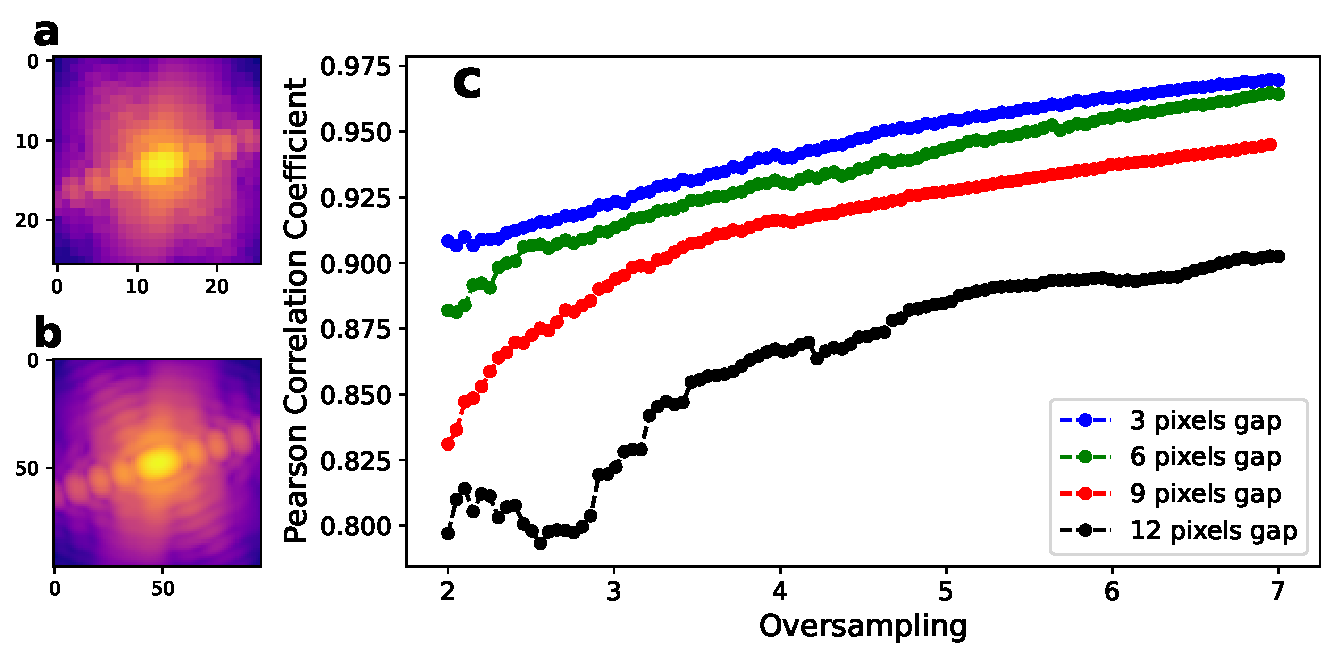
\includegraphics[width=\textwidth]{figures/Inpainting/accuracy_oversampling.pdf}
    \caption{\textbf{Accuracy scores (PCC) of the DL patching model against the oversampling ratio.} \textbf{a)} Simulated 
    diffraction pattern with low oversampling ratio. \textbf{b)} The same pattern simulated on a larger grid for an  
    increased oversampling ratio. \textbf{c)} Pearson Correlation Coefficient (PCC) of the full inpainted diffraction pattern 
    for the four different gap sizes considered. The trend overall confirms the expectations. }
    \label{fig:acc_ovs_3D}
\end{figure}

\section{Results in real space}\label{sec:res_real}

In this section the effects of DL inpainting on the reconstructed objects will be discussed for both simulated and experimental 
data. In particular, the assessment, both qualitatively and quantitatively, of the gap induced artifacts in 
the modulus, phase and strain fields of the reconstructions and their reduction thanks to the DL inpainting are presented. To carry out
these analyses an experimental BCDI dataset acquired at ID01 was considered. The same dataset had already been exploited by 
Carnis \textit{et al.} in 2019 for similar studies on gap-induced artifacts \cite{carnis_towards_2019}. The dataset 
corresponds to the BCDI pattern around the $(\mathbf{111})$ peak of a Pt particle (400 nm in size). 
Similarly to what the authors did, I have kept the modulus of the reconstructed object and set the real space phase
to zero, making it our reference ground-truth object $\textbf{O}$. This measure helps to highlight the gap induced artifacts 
of the phase and strain fields as there is zero-phase 
reference to compare the results with. The corresponding diffraction pattern was then calculated with the Discrete
Fourier transform (DFT) obtaining a complex diffracted amplitude $\mathbf{A}=\mathcal{F}(\mathbf{O})$. A cross-shaped gap was 
subsequently applied to $\mathbf{A}$ and the corresponding object $\mathbf{O}_{gap}$ was calculated with the inverse DFT.
From the same gapped $\mathbf{A}$, the intensity $\mathbf{I} = |\mathbf{A}|^2$ was also ``inpainted'' using our DL model 
and corresponding object $\mathbf{O}_{DL}$ was calculated with the inverse DFT as well, using the ground truth reciprocal 
space phase. The procedure was repeated for four different gap sizes (3, 6, 9, 12 px-wide) matching exactly the cases 
mentioned in the work of Carnis and coauthors. Figure \ref{fig:Carnis_int} shows the projection along the rocking curve 
axis (XY slice in this case) of the ground truth, the gapped and the DL inpainted diffracted intensity for the 
9 pixel-wide gap case. 

Notice that in all cases of Fig \ref{fig:Carnis_int}, there are vertical and horizontal lines of higher intensity not attributable 
to the typical streaks from the truncation rods. These arise from the detector gaps in the original dataset, which are in 
fact responsible for the oscillatory stripe artifacts visible on the object's modulus for all three cases in Fig. 
\ref{fig:Carnis_obj}, ground truth included. The DL inpainting of these original gaps is presented later in Sec. \ref{sec:highres}. 

\begin{figure}[H]
    \centering
    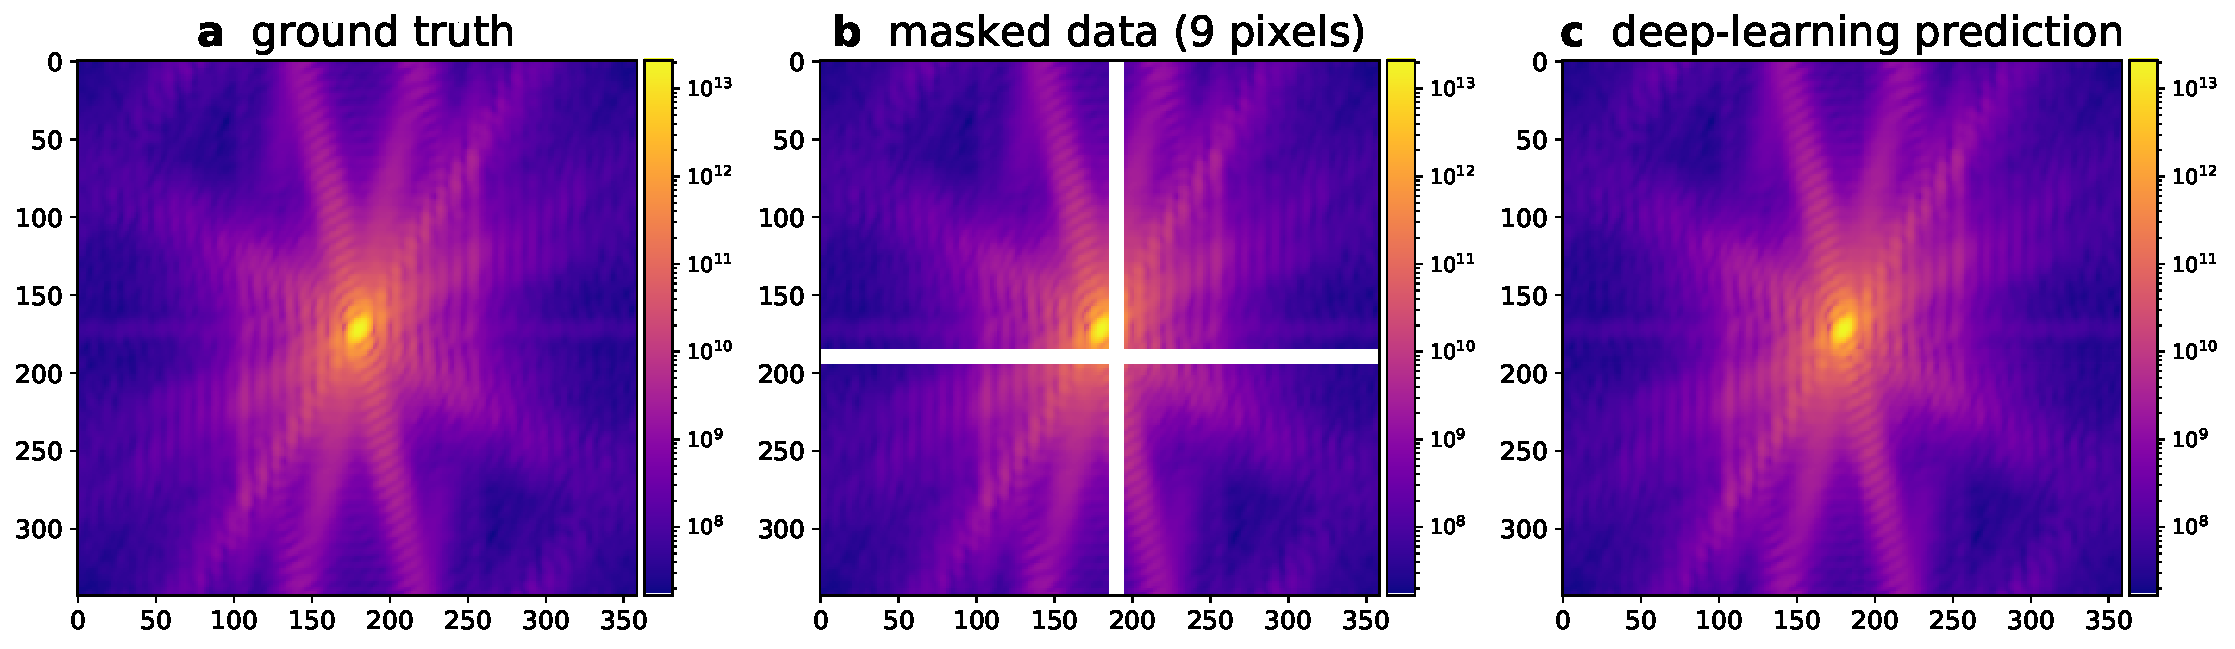
\includegraphics[width=\textwidth]{figures/Inpainting/Carnis_Diffractions_comparison_9px_version2.pdf}
    \caption{\textbf{Projections along the rocking curve axis of the studied diffraction pattern in log scale.} \textbf{a} Ground truth
    pattern obtained from the $|\mathcal{F}(\mathbf{O})|^2$. \textbf{b} Pattern with a 9 pixel-wide cross shaped gap. The position close to the center of 
    the peak is experimentally unlikely but here it allows us to enhance the artifacts in the reconstructions. \textbf{c} 
    Corresponding DL inpainted BCDI pattern. The presence of aliasing can be seen  due to the DFT calculation as compared 
    to the correct kinematic sum. This effect is however not relevant for the scope of these analyses.}
    \label{fig:Carnis_int}
\end{figure}

\begin{figure}[H]
    \centering
    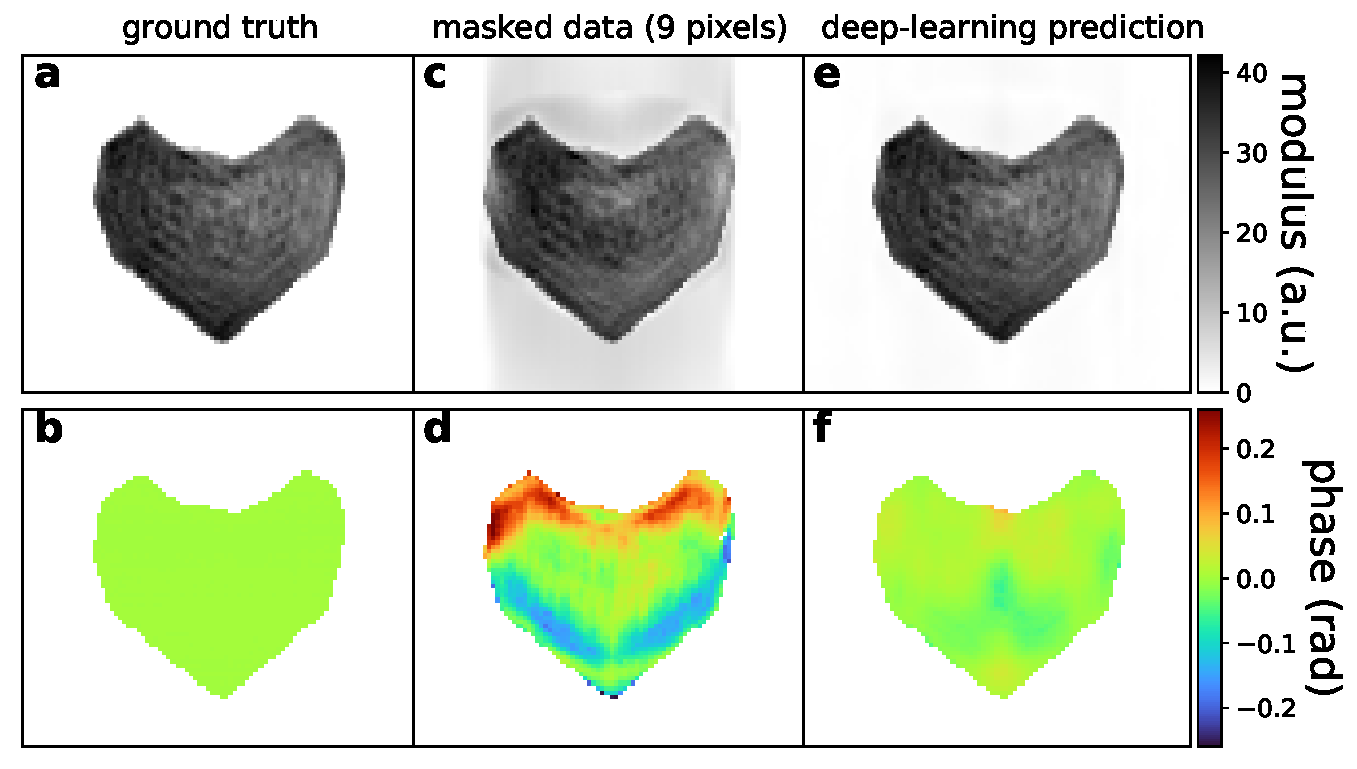
\includegraphics[width=\textwidth]{figures/Inpainting/Real_space_comparison_axis0-1.pdf}
    \caption{\textbf{Reconstructed objects (central slice)}.\textbf{a-b} XY central slice of ground truth modulus 
    and phase obtained from the reconstruction 
    of an experimental gap-less dataset. The object's phase has been set to zero artificially after the reconstruction for 
    better assessment of the gap-induced artifacts. \textbf{c-d} Modulus and phase of  
    $\mathbf{O}_{gap}$, the object obtained from the inverse DFT of the diffraction pattern (with reconstructed reciprocal 
    space phase) with a 9 px-wide cross-shaped gap placed as shown in Fig.\ref{fig:Carnis_int}. \textbf{e-f} Modulus 
    and phase of $\mathbf{O}_{DL}$, the object reconstructed from the DL-inpainted diffraction pattern. The phase of this 
    last object shows reduced artifacts with respect to \textbf{d}.}
    \label{fig:Carnis_obj}
\end{figure} 

Figure \ref{fig:Carnis_obj} illustrates instead the central slice (XY) of the reconstructed objects for 
the three cases. It is evident that while $\mathbf{O}_{gap}$ shows significant abnormalities in both modulus and phase, 
$\mathbf{O}_{DL}$ is much closer to the ground truth. In particular one can notice that the gap plane, horizontal in the 
XY plane, induces artifacts along its perpendicular direction. The result is indeed a stripe of non-zero modulus outside 
the support and, most importantly, an overall phase variation of 0.4 radians along the vertical direction. This phase variation
results in an error of $\pm 7$ pm in the lattice displacement field for the $111$ Pt reflection, with more intensity around the 
surface. These artifacts are particularly problematic in the cases of (electro-)catalytic experiments \cite{atlan_imaging_2023}
or in situ gas experiments \cite{Ulvestad2015, Kim2018,PhysRevLett.123.246001, Abuin2019, Dupraz_2022}, 
where the particle's surface is primarily involved in the reaction and one could follow the process by monitoring the evolution
of the strain in that region. As one could expect the artifacts become more severe as the gap size increases. Fig.\ref{fig:Carnis_allgaps} depicts 
the phases of $\mathbf{O}_{gap}$ and $\mathbf{O}_{DL}$ for the different gap sizes considered in this study while 
Fig.\ref{fig:Carnis_allgaps_strain} the strain distribution in the XY plane. 

\begin{figure}[H]
    \centering
    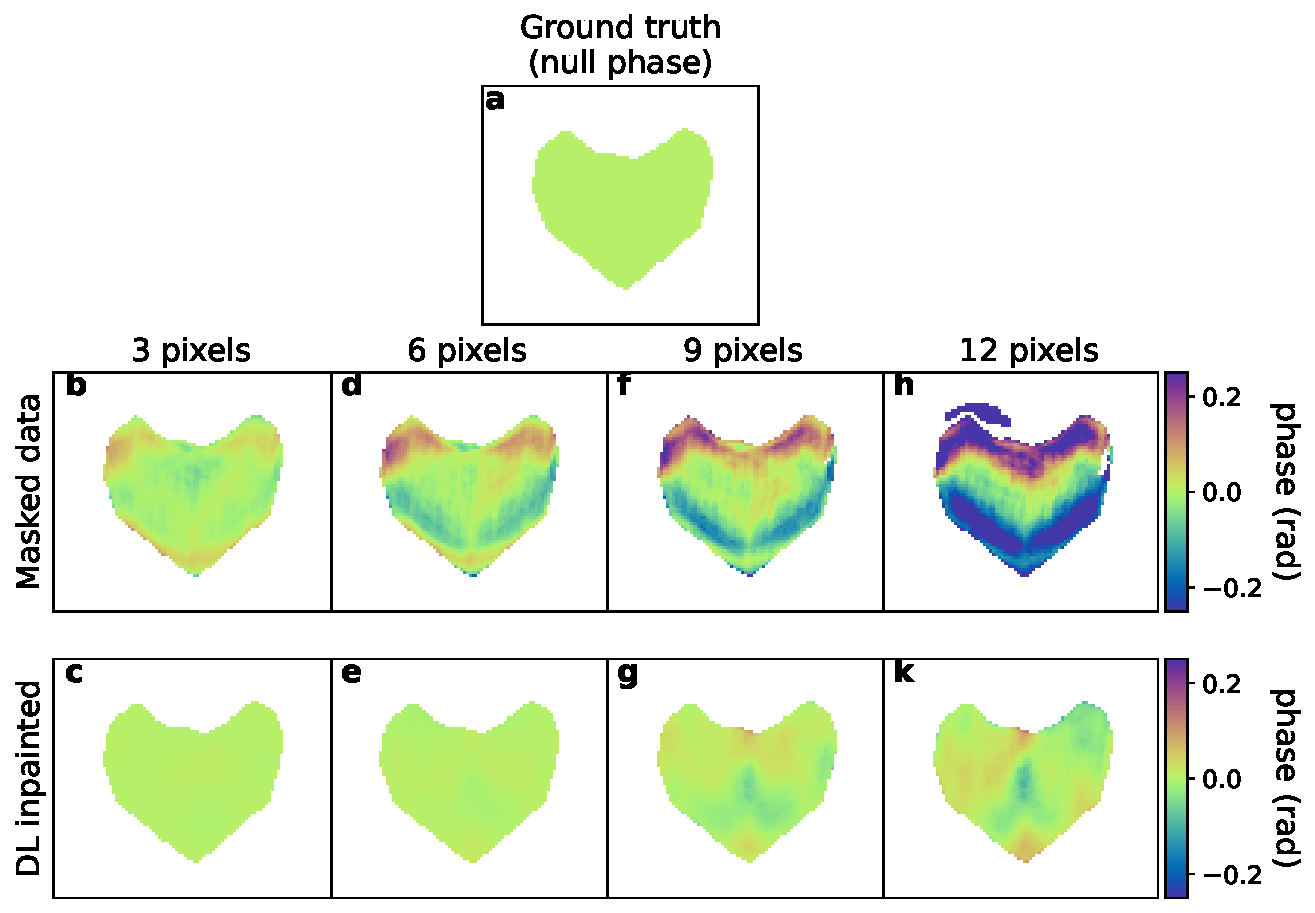
\includegraphics[width=\textwidth]{figures/Inpainting/strain_comparison_allGaps-1.pdf}
    \caption{\textbf{Comparison of the phase artifacts vs gap size.} XY central slice of the phase of $\mathbf{O}_{gap}$ 
    for different gap sizes (\textbf{b-d-f-h}), and phase of the corresponding $\mathbf{O}_{DL}$ (\textbf{c-e-g-k}). 
    The comparison with the ground truth null phase (\textbf{a}) shows a significant increment of the artifacts in  
    $\mathbf{O}_{gap}$ with the gap size. On the contrary, in $\mathbf{O}_{DL}$ artifacts are severely reduced for 
    all gap sizes. }
    \label{fig:Carnis_allgaps}
\end{figure}


\begin{figure}[H]
    \centering
    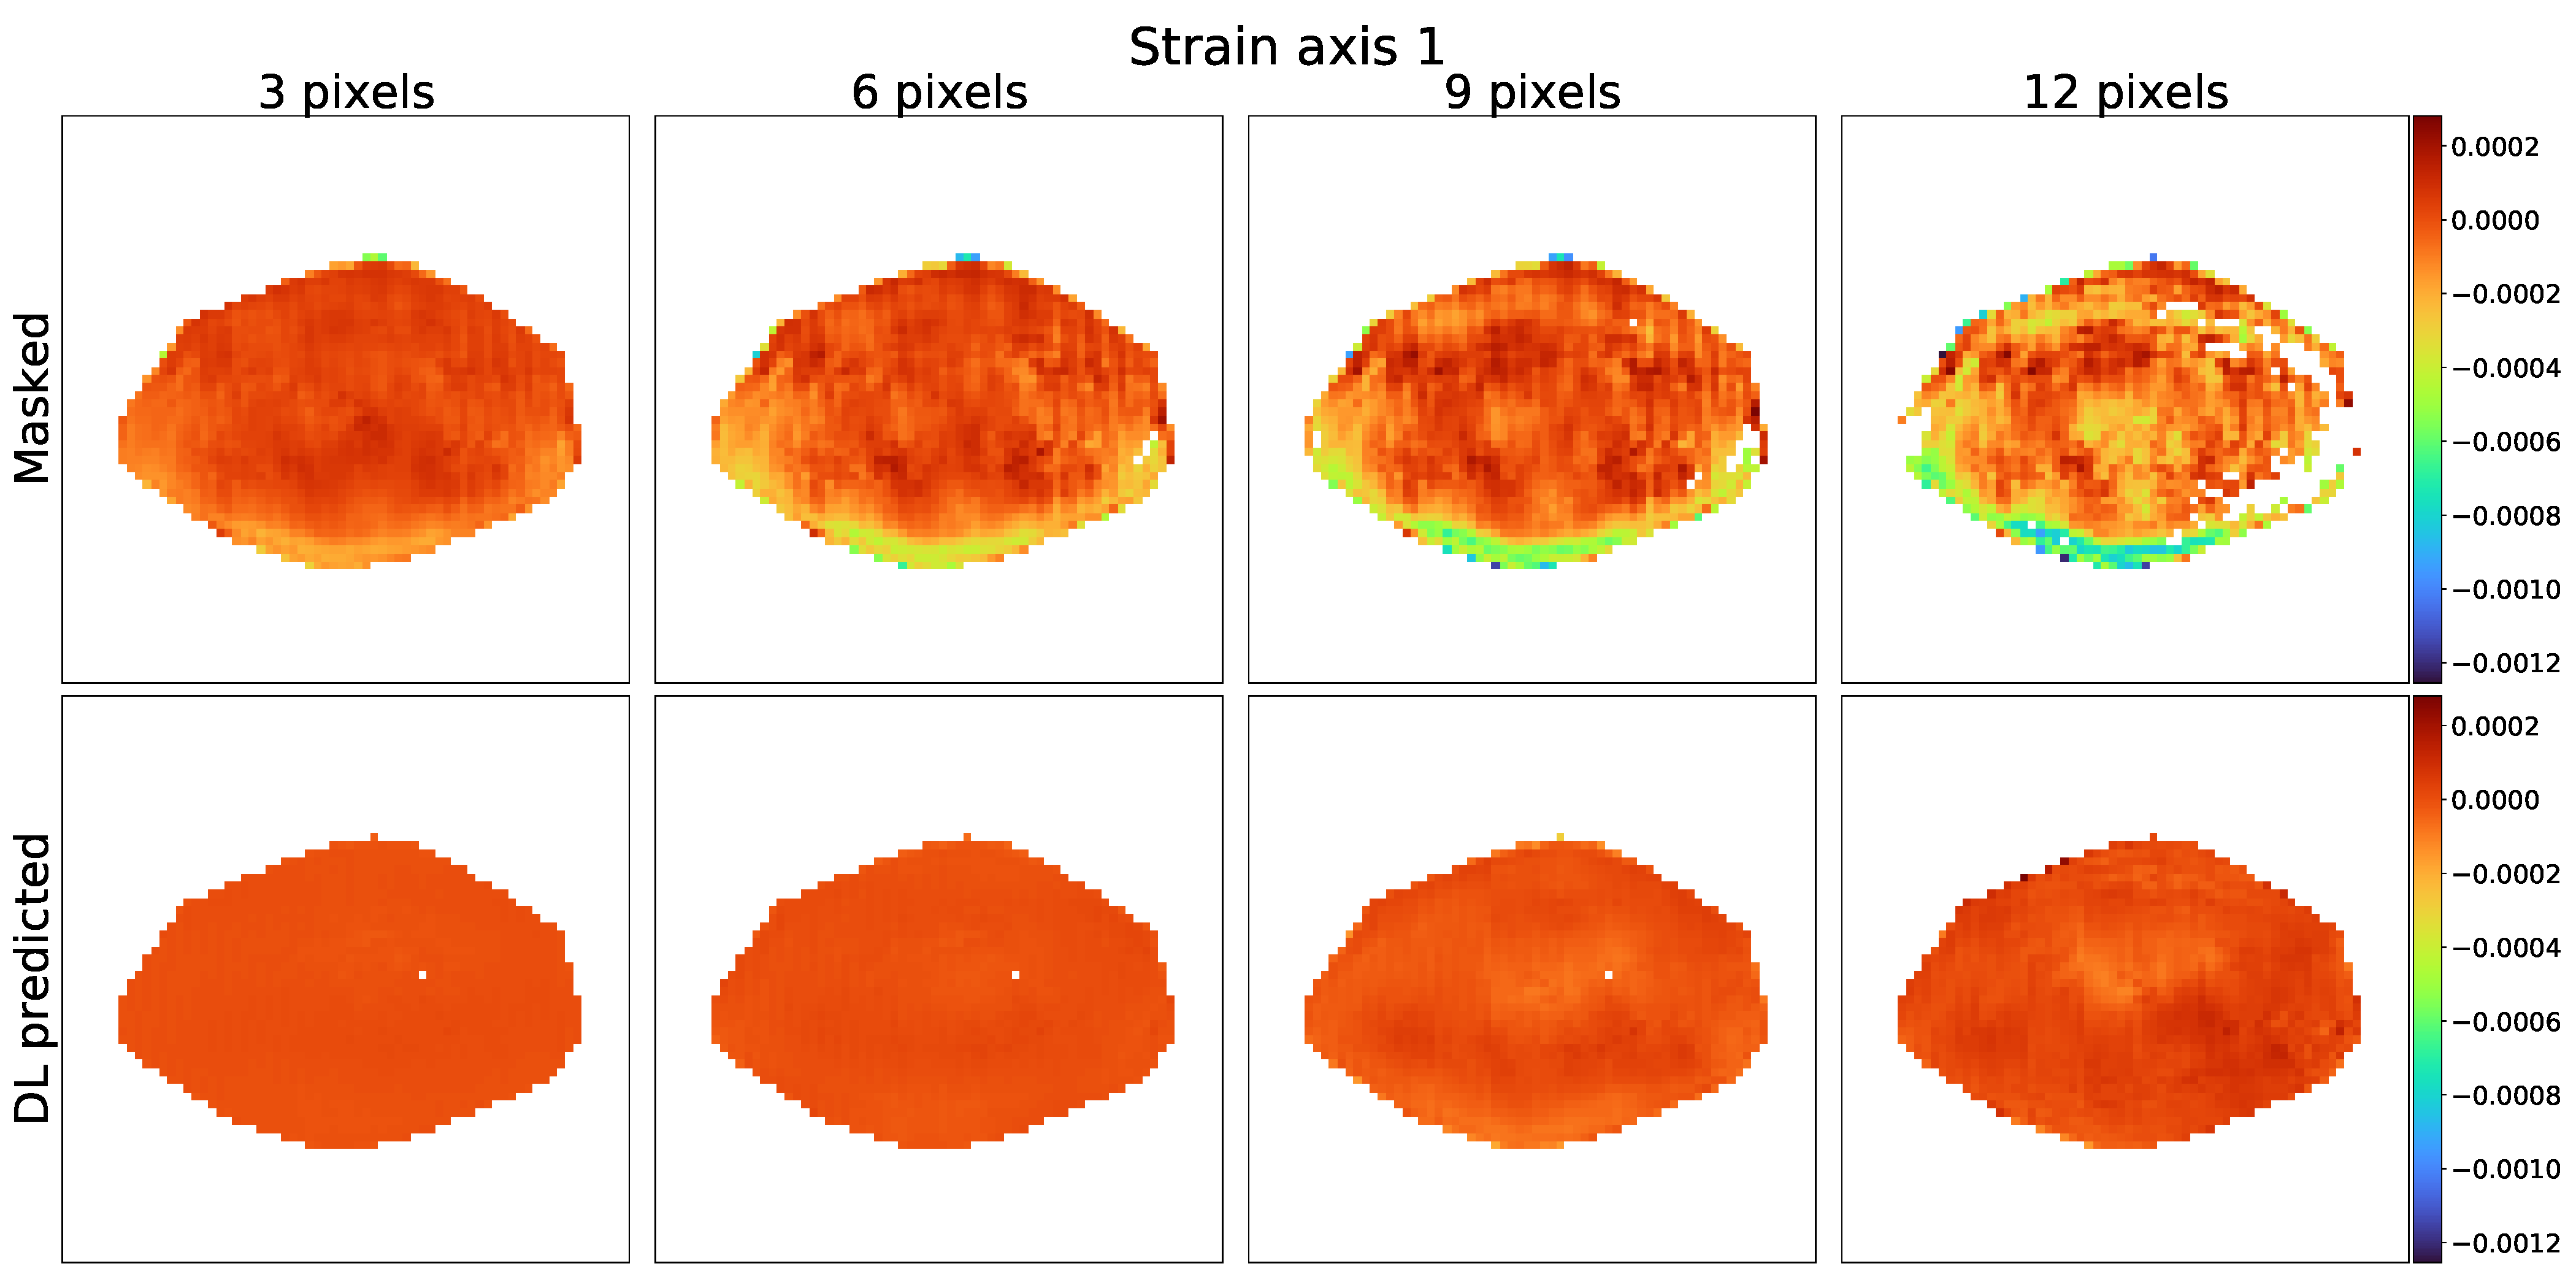
\includegraphics[width=\textwidth]{figures/Inpainting/strain_comparison_allGaps.pdf}
    \caption{\textbf{Comparison of the strain vs gap size.} XZ central slice of the strain distribution for of $\textbf{O}_{gap}$
    (first row) and $\textbf{O}_{DL}$ (second row) for different gap sizes.}
    \label{fig:Carnis_allgaps_strain}
\end{figure}

The deviation from the ground truth zero value of the retrieved strain for both $\mathbf{O}_{gap}$ and $\mathbf{O}_{DL}$
can be measured with the root mean squared error (RMSE) across all the different gap sizes. This calculation was already
proposed in the aforementioned work of Carnis and coauthors in which the results were plotted in Fig.4. We have reproduced
a similar figure adding the results of our DL model (Fig.\ref{fig:Carnis_std}). The trend of the strain RMSE 
resembles the curve shown in \cite{carnis_towards_2019}, increasing significantly with the gap size 
while the DL equivalent curve lies below, dampening the error by approximately a factor 5. 

\begin{figure}[H]
    \centering
    \begin{subfigure}{0.42\textwidth} 
        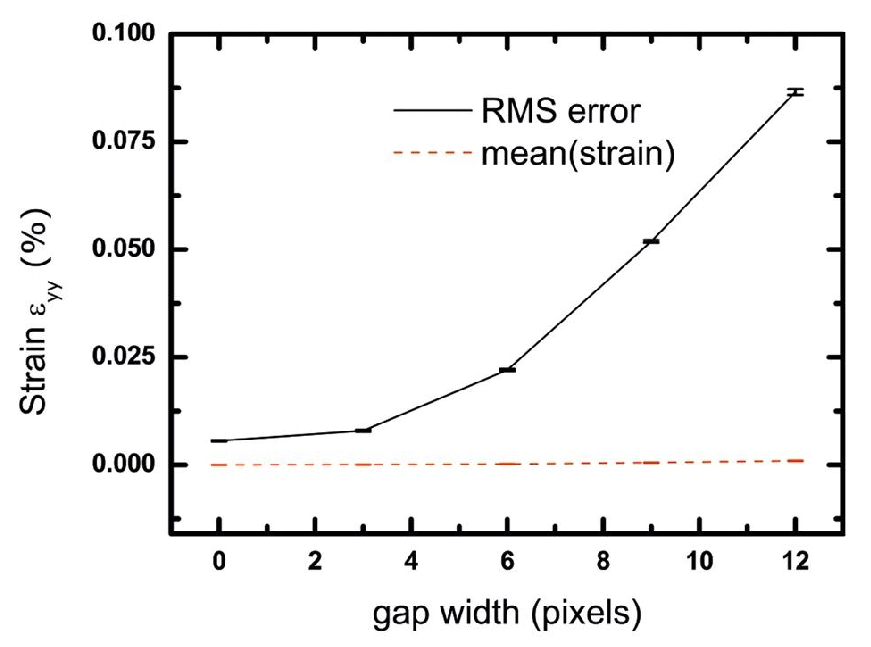
\includegraphics[width=\linewidth]{figures/Inpainting/Carnis_plot_paper.pdf}
        \caption*{}
    \end{subfigure}
    \hfill
    \begin{subfigure}{0.52\textwidth}
        \centering
        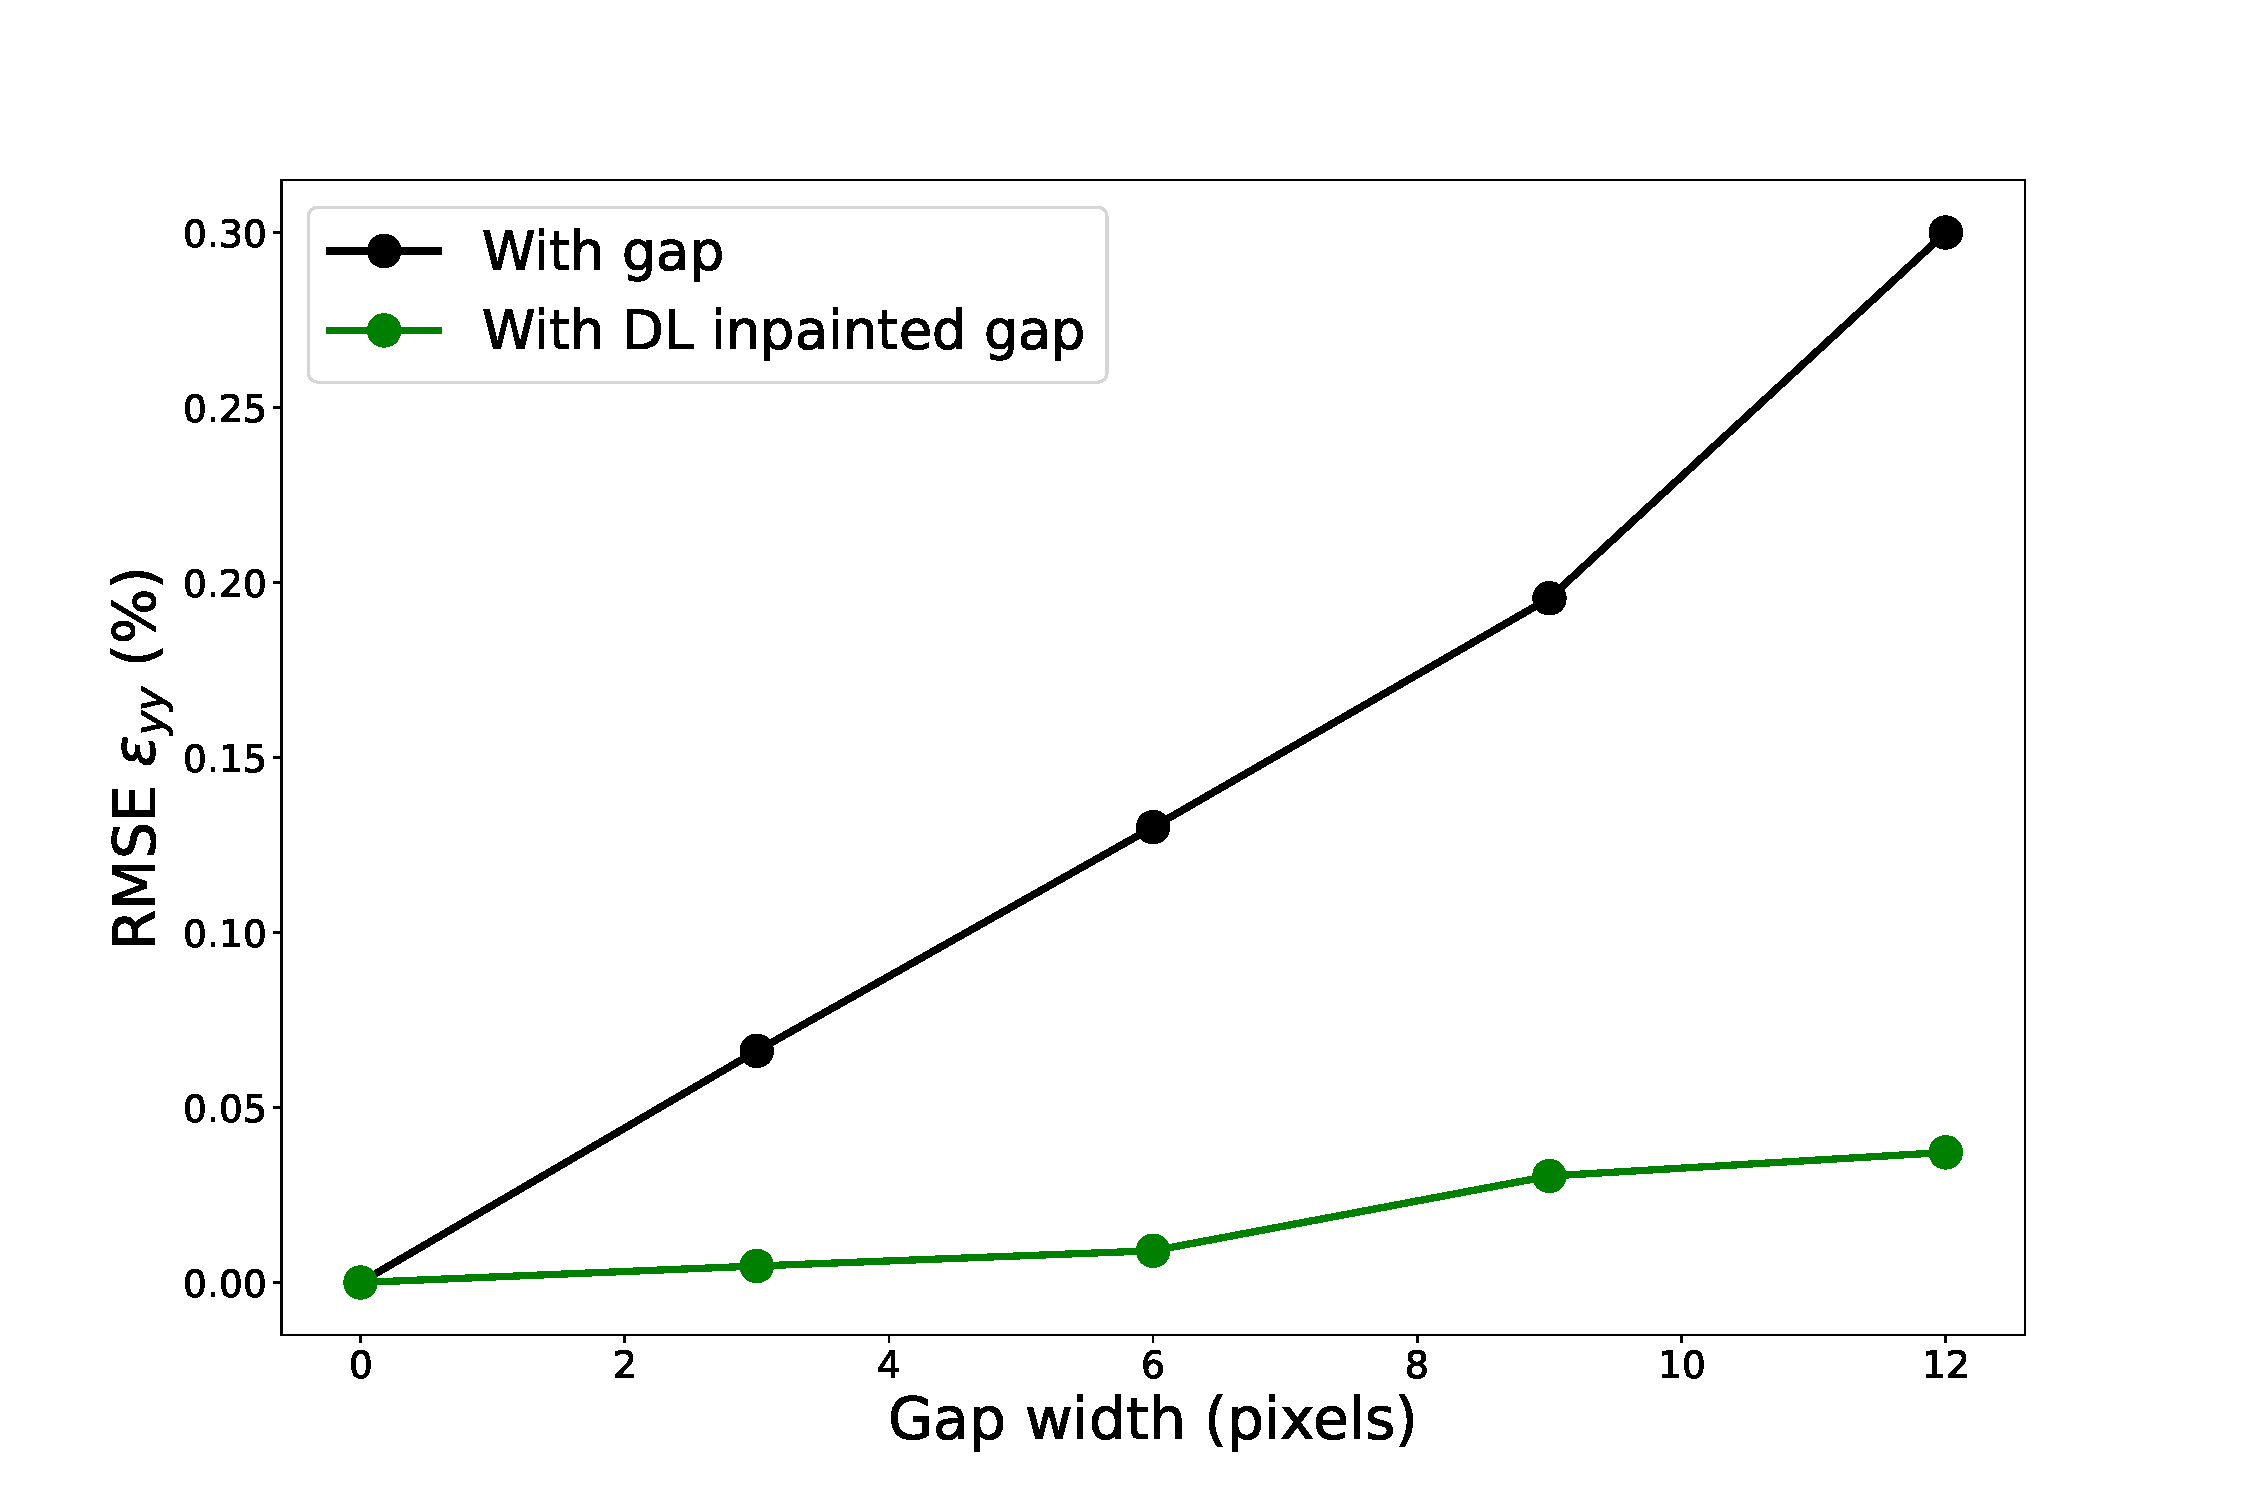
\includegraphics[width=\linewidth]{figures/Inpainting/std_strain_comparison.pdf}
        \caption*{}
    \end{subfigure}
    \caption{\textbf{RMSE of the strain field versus gap size}(\textbf{Left}) The plot realized by Carnis \textit{et al.} in 
    \cite{carnis_towards_2019} depicts the RMSE of the $\varepsilon_{yy}$ strain component for the objects reconstructed 
    from gapped diffraction patterns with different gap-size. The mean strain around zero corresponds to the null object's phase 
    set artificially. (\textbf{Right}) Plot of the RMSE of the $\varepsilon_{yy}$ strain component versus same gap-size 
    as \textbf{(Left)} for gapped (blue line) and DL inpainted (orange line) diffraction patterns. }
    \label{fig:Carnis_std}
\end{figure}

% \begin{figure}[H]
%     \centering
%     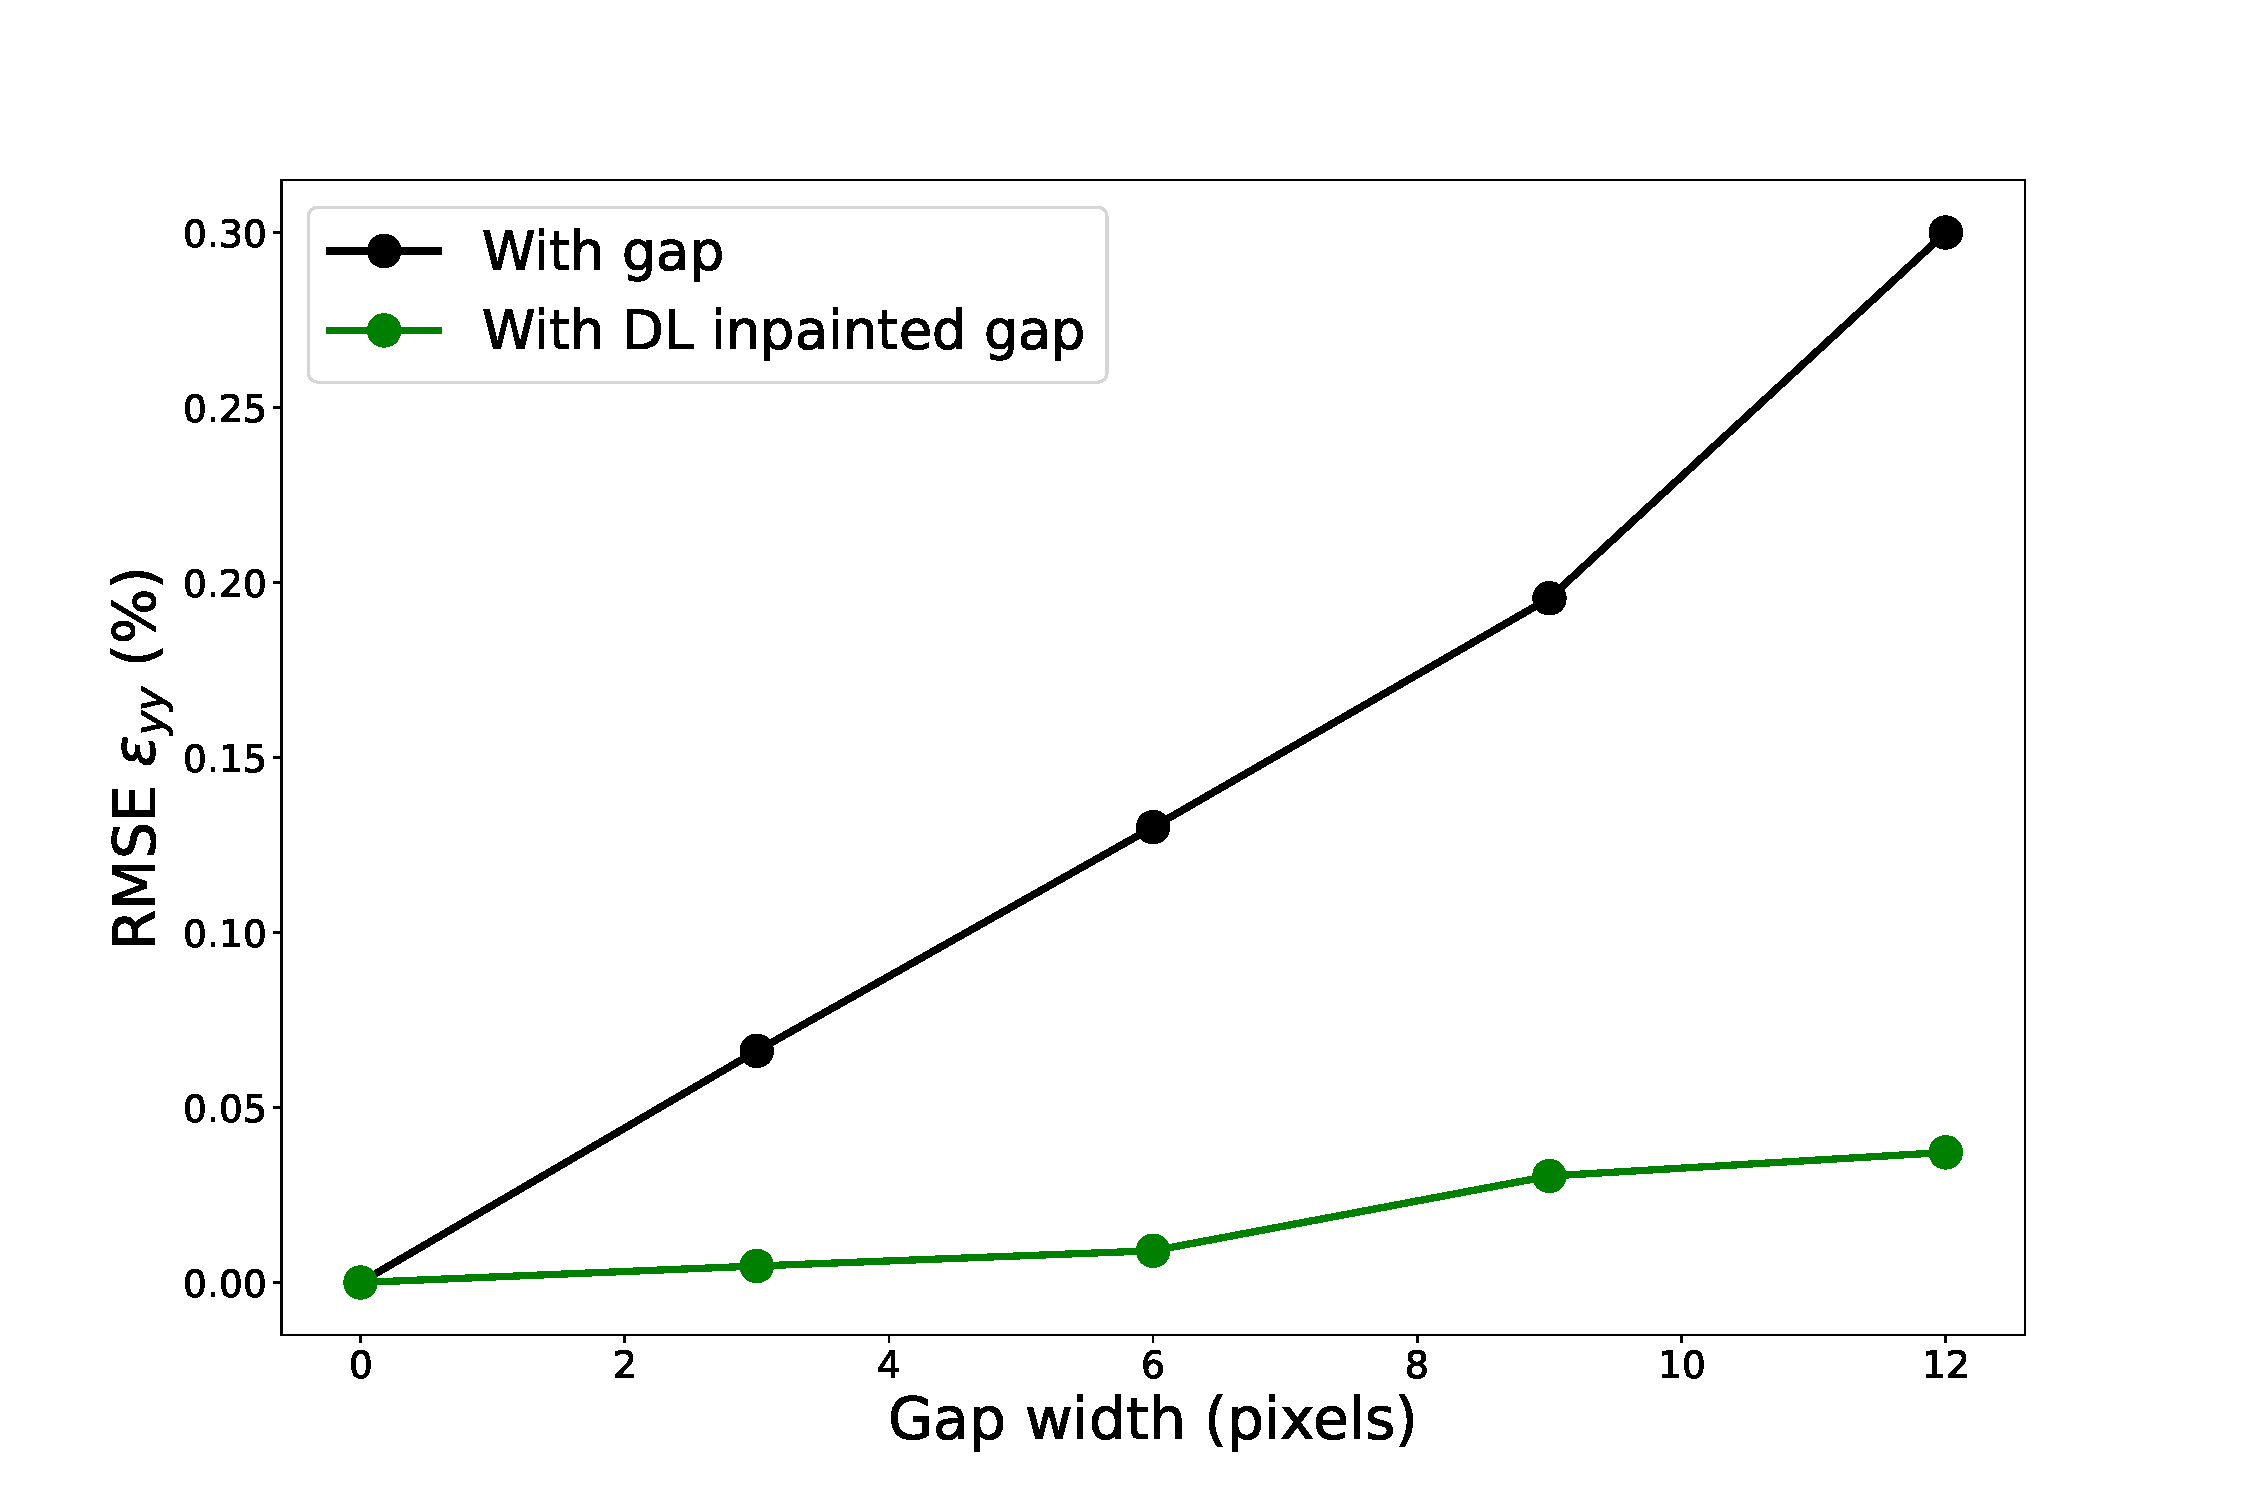
\includegraphics[width=\textwidth]{figures/Inpainting/std_strain_comparison.pdf}
%     \caption{RMSE of the strain field versus gap size. For both cases of masked and DL inpainted diffraction
%     patterns. For all gap sizes, the DL inpainted diffraction patterns yield a smaller error.
%     }
%     \label{fig:Carnis_std}
% \end{figure}

% \begin{figure}[H]
%     \centering
%     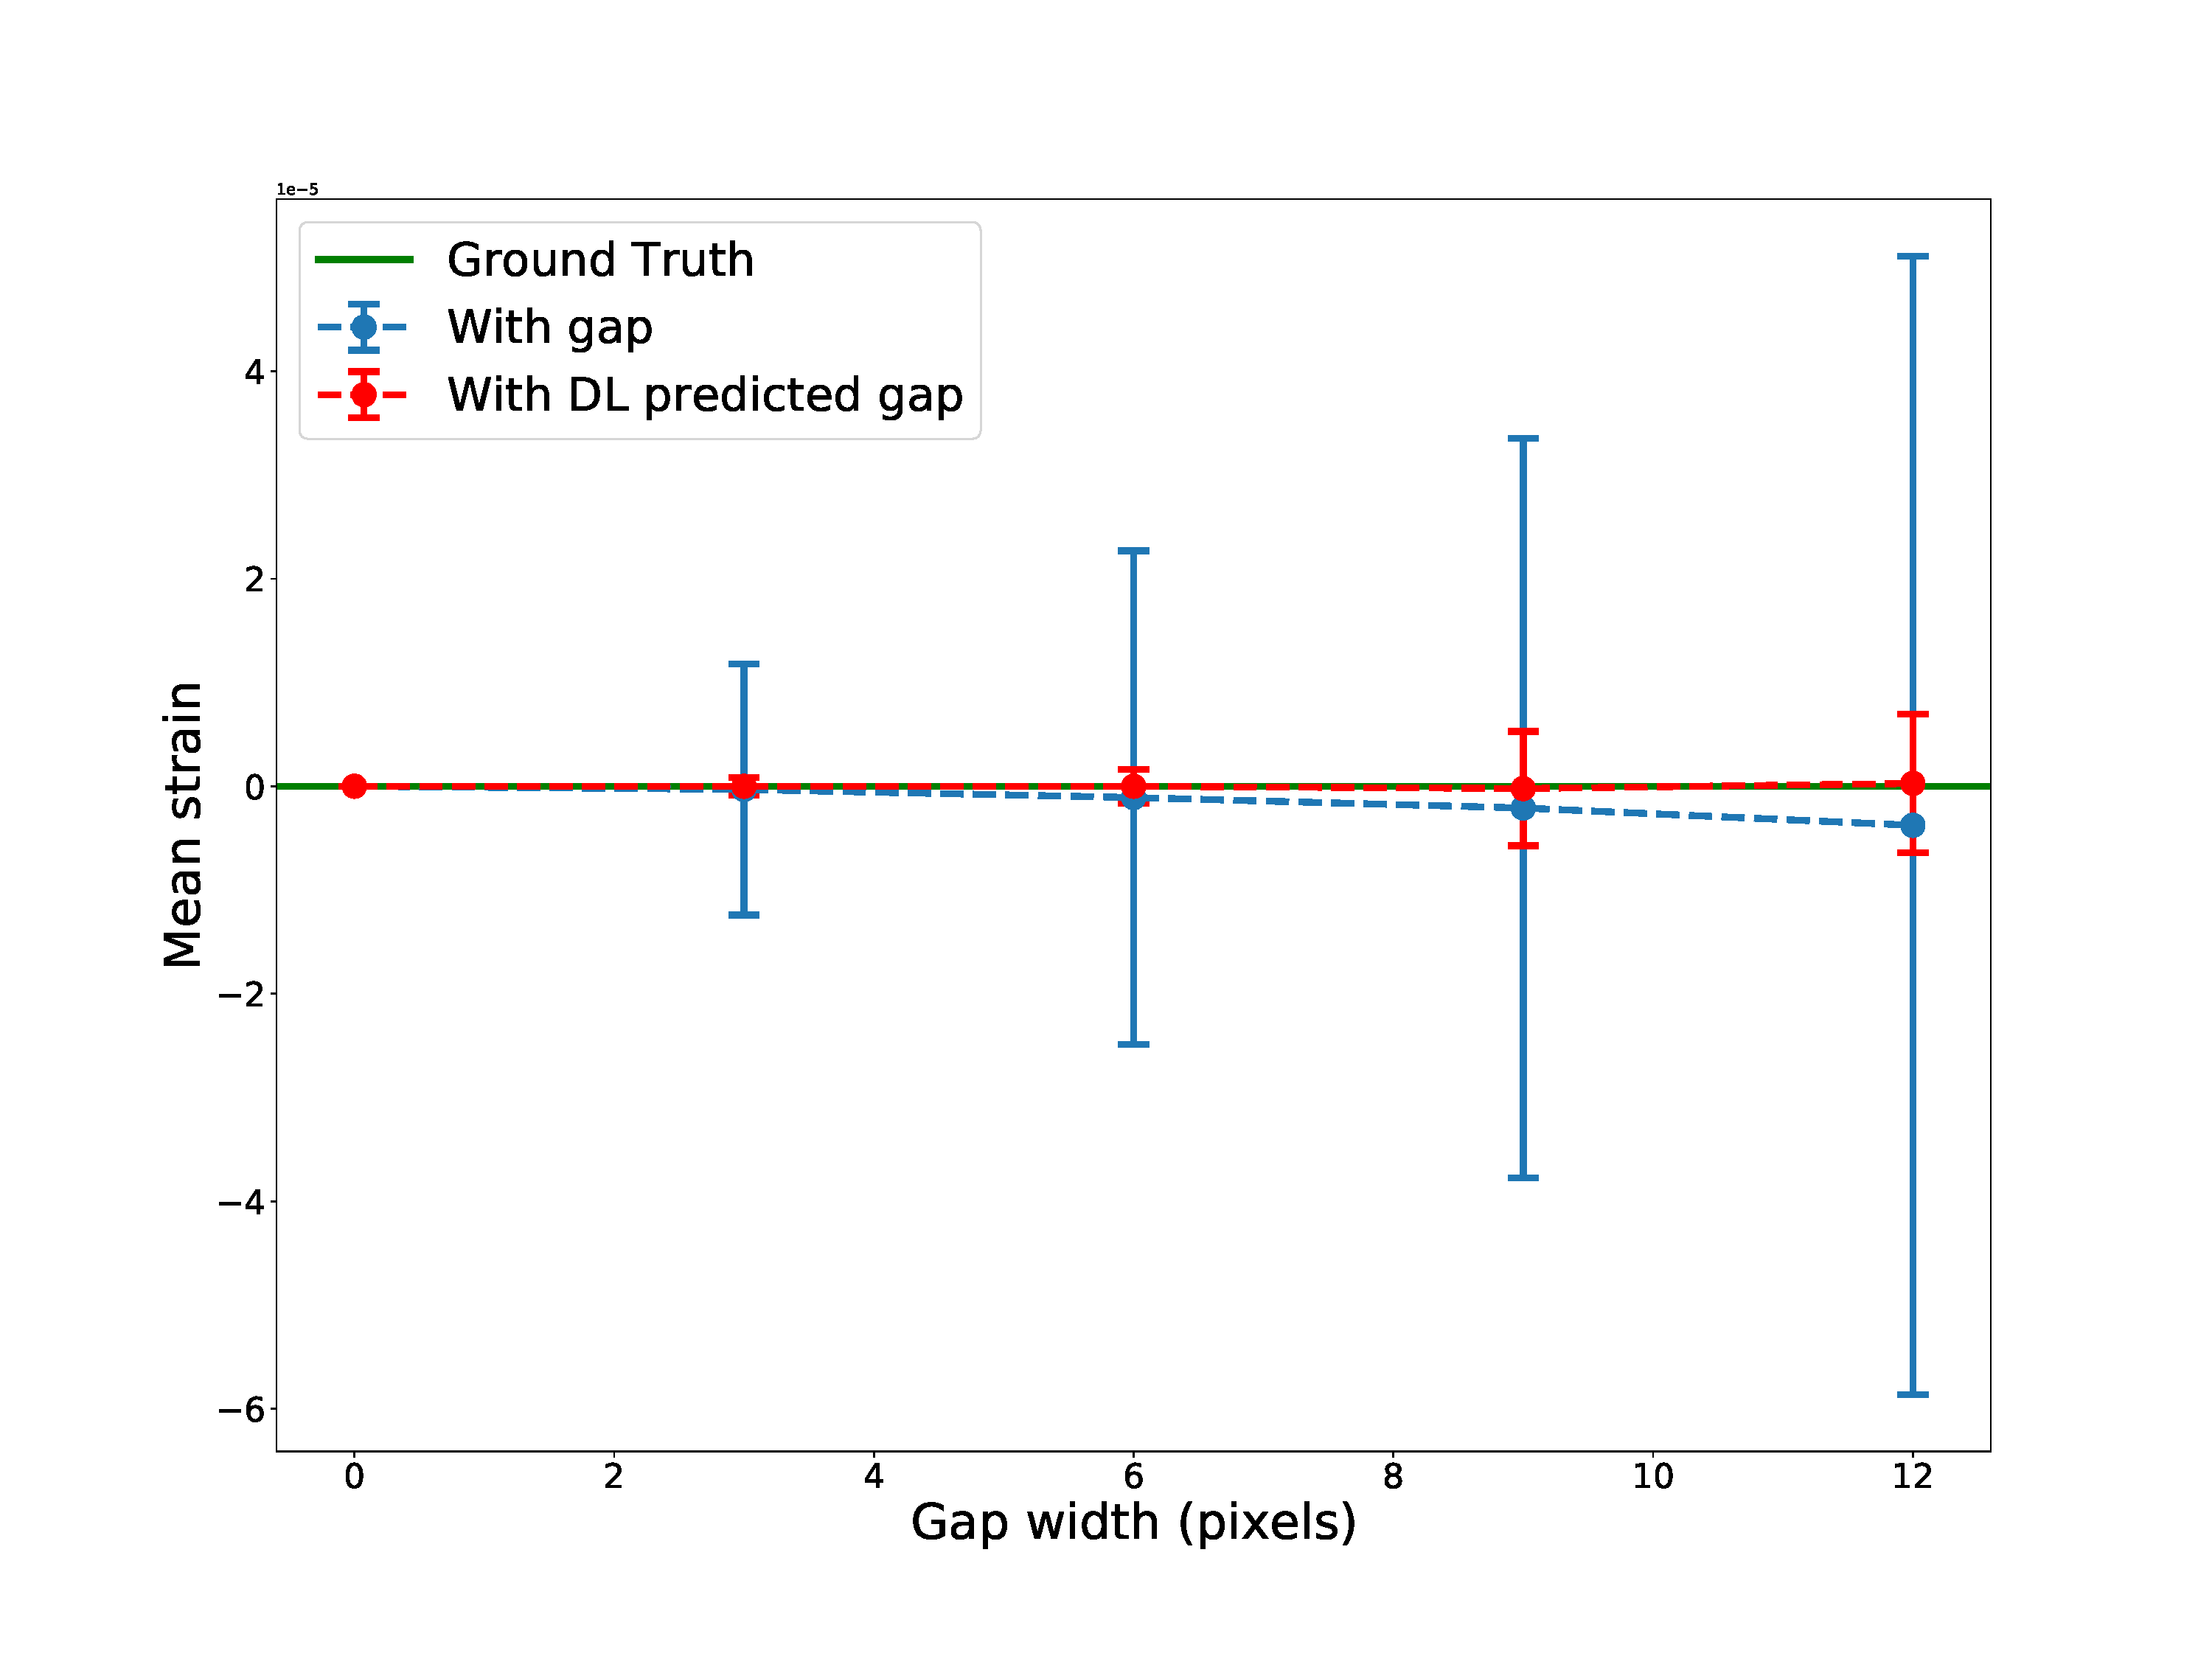
\includegraphics[width=\textwidth]{figures/Inpainting/avg_strain_comparison-1.pdf}
%     \caption{\textbf{Mean value and RMSE of the strain field versus gap size.} The mean strain calculated for the 
%     $\mathbf{O}_{gap}$ and $\mathbf{O}_{DL}$ (blue and orange dashed lines respectively) versus different 
%     gap sizes. Error bars represent the RMSE. $\mathbf{O}_{DL}$ mean strain is closer to the ground truth zero value 
%     for all gaps than the corresponding results for $\mathbf{O}_{gap}$ which deviates from the mean as the gap size increases.
%     As shown in Fig. \ref{fig:Carnis_std}, the RMSE of $\mathbf{O}_{DL}$ is over five times smaller than that of
%      $\mathbf{O}_{gap}$.}
%     \label{fig:Carnis_avg}
% \end{figure}

\subsection{DL inpainting for high resolution BCDI}\label{sec:highres}

As anticipated in the introduction to the chapter, the most prominent case in which a BCDI datasets is affected by 
a detector gap is a ``high-resolution'' dataset. The acquired data here extend for large $q$ ranges in all
directions resulting in parts of the diffracted signal that cross a region 
on the detector with a vertical or horizontal gap, hence the need for gap-inpainting. All the more so, it is convenient to use a
patching approach since treating the full volume would be computationally too expensive. Moreover, any binning or interpolation
to smaller sizes will induce information loss, and is not advised. \\
An example of high-resolution BCDI dataset of this type is the one we have used so far from the work of Carnis and coauthors. 
The original dataset is indeed a large ($256\times300\times300$ pixels) array that contains a cross-shaped, 6 pixel-wide 
gap. Here we show how the artifacts can change depending on the type of masking of the gaps is chosen during the phasing
and how our DL model can outperform these methods. 
A common approach, when using PyNX software, is to mask the gap such that those pixels don't contribute during the 
phasing and are left free to evolve (\textbf{a}). Moreover, one could mask only near the intensity streaks affected 
by the gap (\textbf{b}) or simply leave the gap with zeros and remove the contribution of the gap voxels during the whole phasing
(\textbf{c}). These strategies have been used during the phasing of the cited Pt diffraction pattern and the results 
in object space compared with that obtained from the DL inpainted pattern. The results, illustrated in Figs. \ref{fig:high_res_Icalc}
- \ref{fig:high_res_obj}, show that the amount of oscillatory artifacts progressively decreases as we go from method 
\textbf{a} to \textbf{c}, proving the DL inpainting to be the optimal method among them. 

\begin{figure}[H]
    \centering
    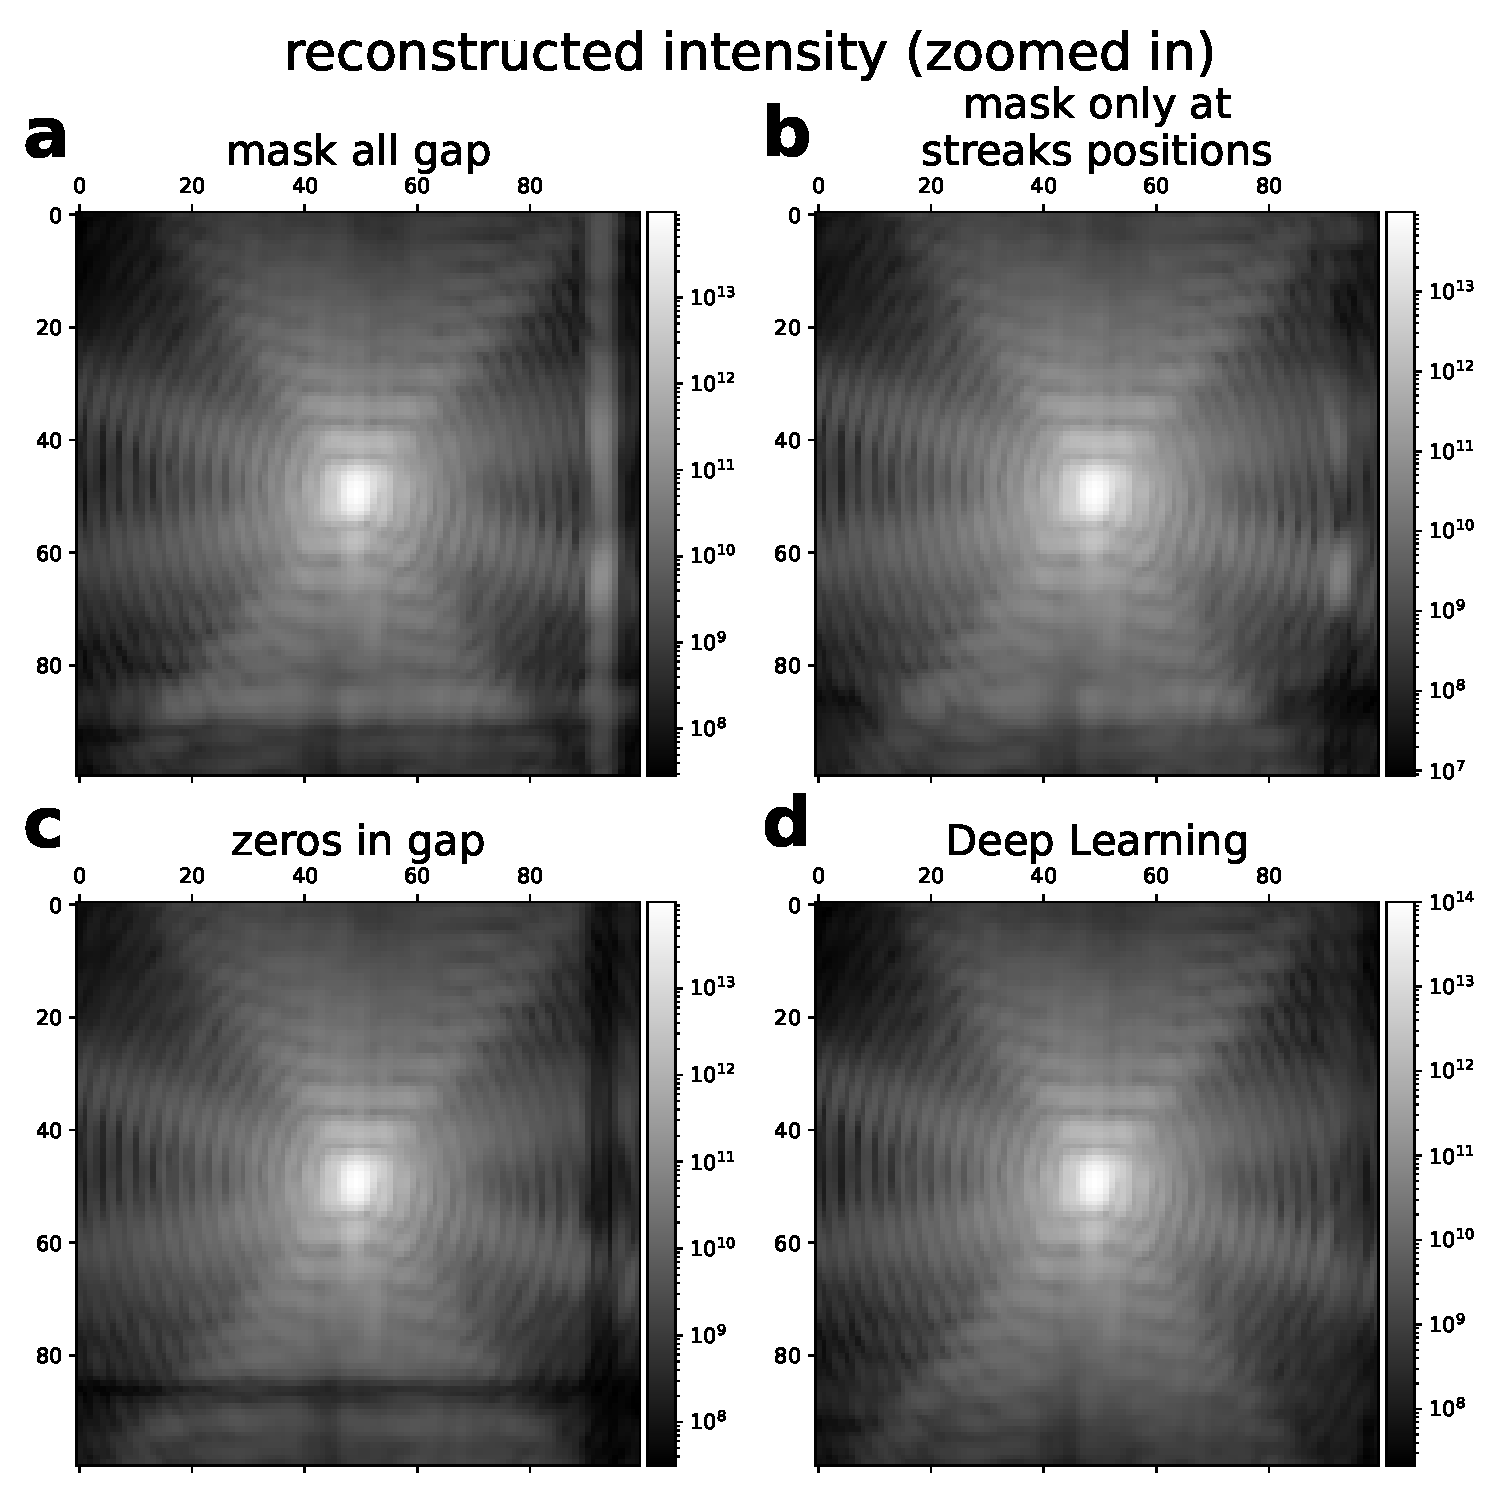
\includegraphics[width=\textwidth]{figures/Inpainting/reconstructed_intensity_zoom_jerome.pdf}
    \caption{Zoom on the projection along the rocking curve axis of the Pt BCDI pattern in Fig.\ref{fig:Carnis_int} 
    calculated from the reconstructed object obtained with PyNX software using \textbf{(a)} a mask on the gaps, 
    \textbf{(b)} a mask on the streaks only, leaving zeros inside the gaps \textbf{(c)} and inpainting the gaps with 
    the DL model \textbf{(d)}. Inside the regions where the mask was applied the intensity is free to vary throughout 
    the PR iterations. }
    \label{fig:high_res_Icalc}
\end{figure}

\begin{figure}[H]
    \centering
    \begin{subfigure}{0.47\textwidth} 
        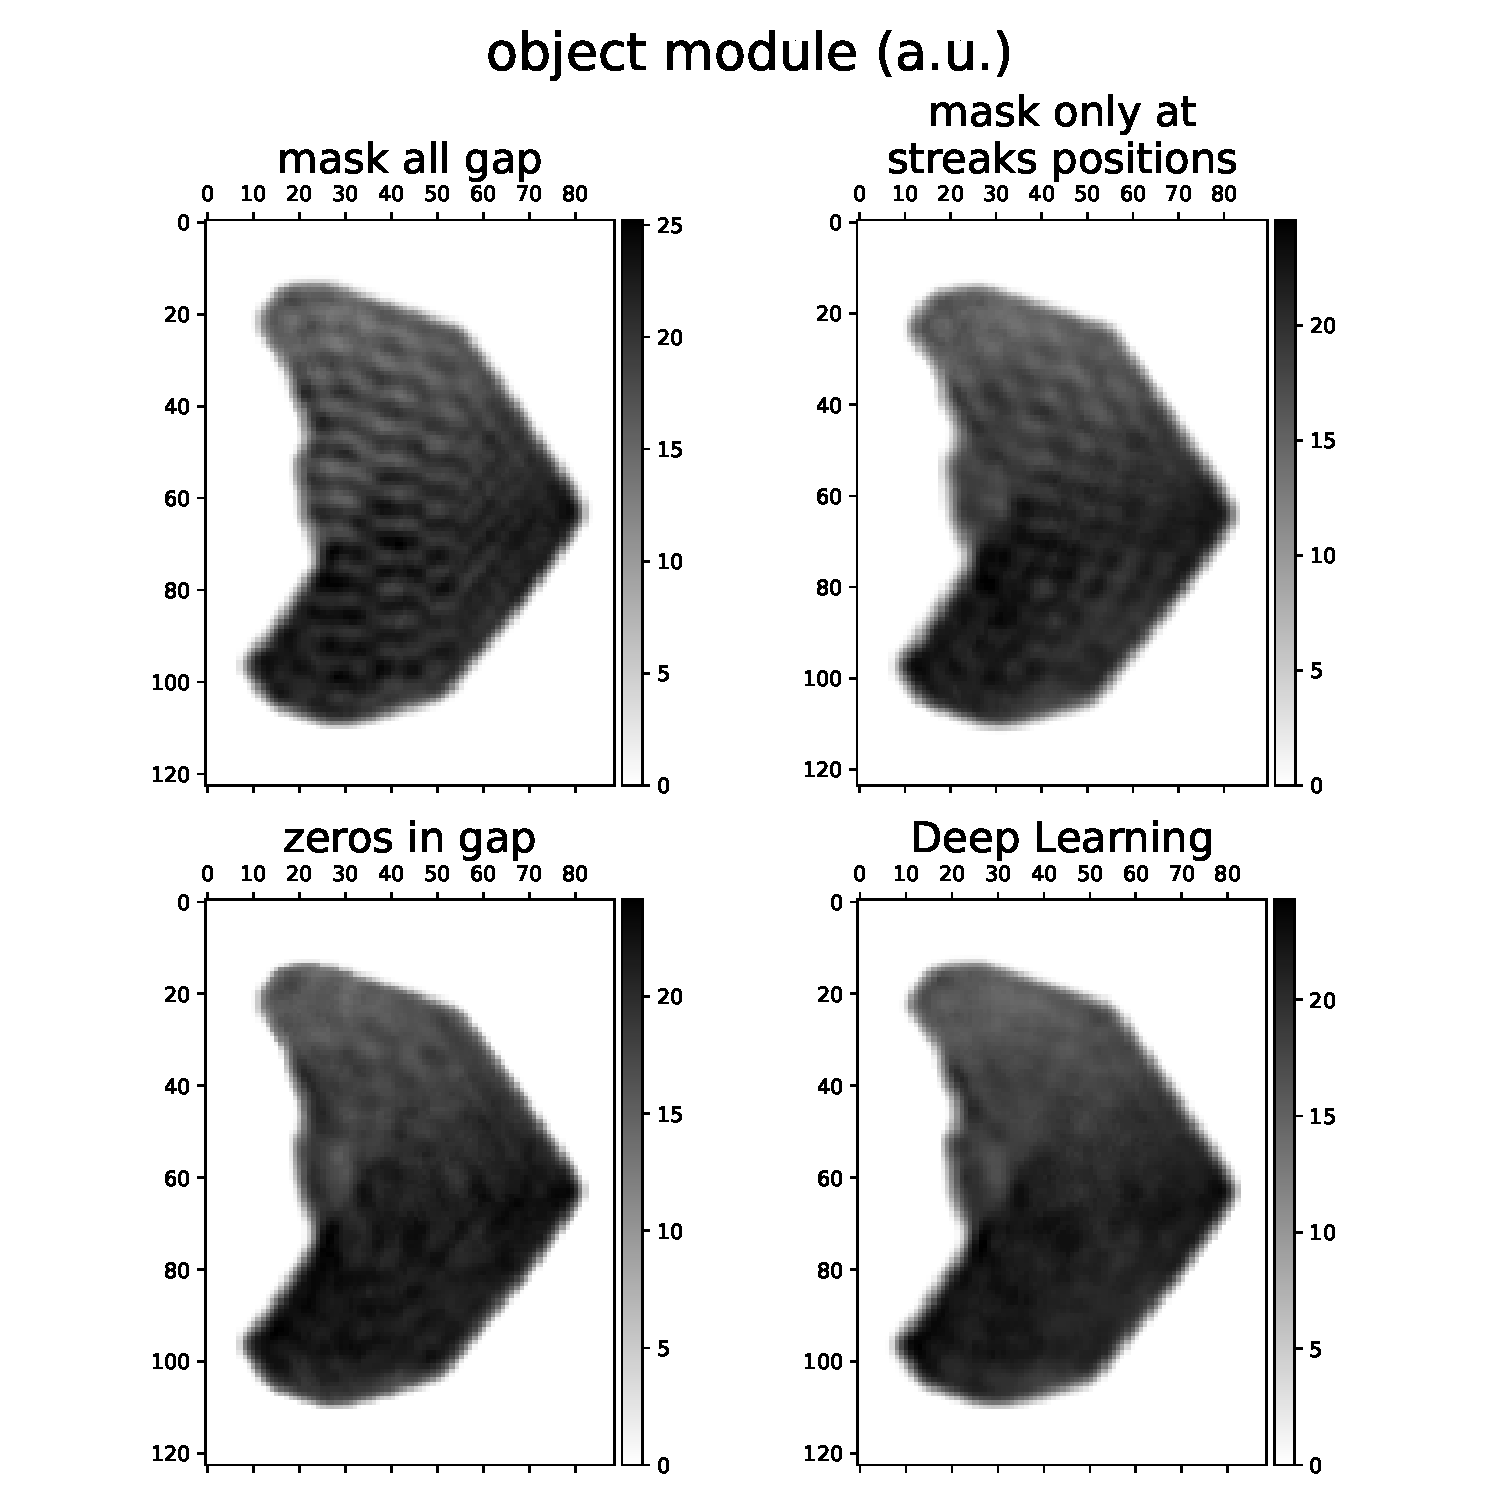
\includegraphics[width=\linewidth]{figures/Inpainting/object_module_jerome.pdf}
        \caption*{}
    \end{subfigure}
    \hfill
    \begin{subfigure}{0.47\textwidth}
        \centering
        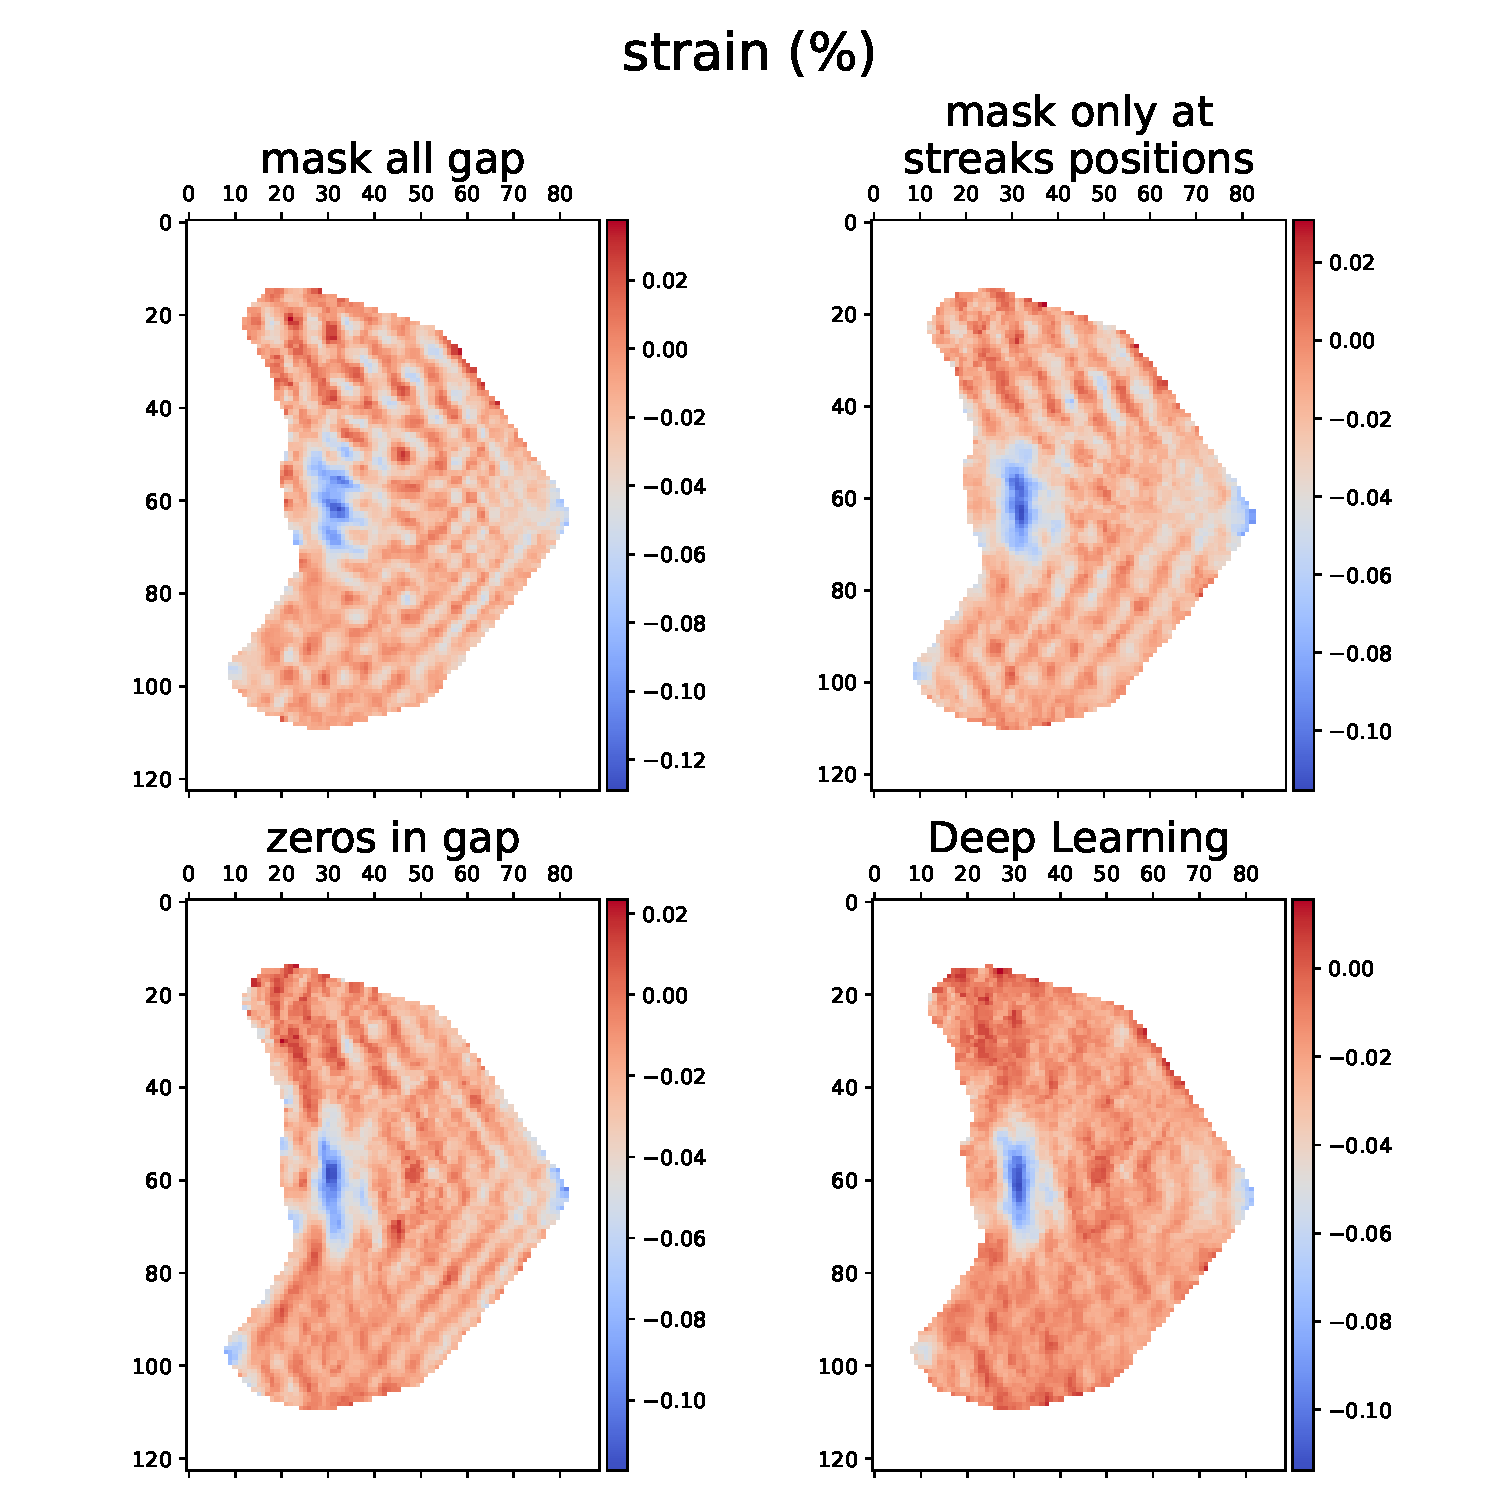
\includegraphics[width=\linewidth]{figures/Inpainting/object_strain_jerome.pdf}
        \caption*{}
    \end{subfigure}
    \caption{Modulus (\textbf{Left}) and strain (\textbf{Right}) of the object's reconstructions for each case mentioned 
    above in Fig. \ref{fig:high_res_Icalc}. The oscillatory artifacts are smallest for the object obtained after DL 
    inpainting (bottom right corner on both left and right images).}
    \label{fig:high_res_obj}
\end{figure}

\section{Fine-tuning}\label{sec:finetuning}
For those cases in which the DL model does not yield satisfactory results when inpainting a new experimental BCDI pattern 
a fine-tuning of the model was conceived in order to improve the accuracy of the prediction. This fine-tuning is enabled by the 
patching approach as it consists of a secondary short training of the general model on a small dataset made of portions 
extracted from the new BCDI pattern to be inpainted.
In particular, after loading the gap affected BCDI pattern, 2000 portions were randomly cropped out of it, paying attention
not to include the gap region. The model has been trained for the corresponding gap width for 2 epochs with a learning 
rate of $ 10^{-5}$  and batches of 32 images ($\sim 2$ mins on a
NVIDIA Tesla V100-SXM2 GPU with 32GB RAM ). Biasing the
model to fit the features of that specific diffraction pattern (oversampling ratio, particle shape, noise level, fringes shape)
better results can were obtained on the real gap. An example is shown in Fig.\ref{sec:finetuning}. There, the general DL model
was not able to predict the fringes with the correct periodicity inside the gap. After the fine-tuning instead, the model 
properly recovers the fringes improving the accuracy. 
This fine-tuning technique is a further example of the advantage of using a patching approach and its usage depends
on the user judgement on the quality of the general model inpainting. 

\begin{figure}[H]
    \centering
    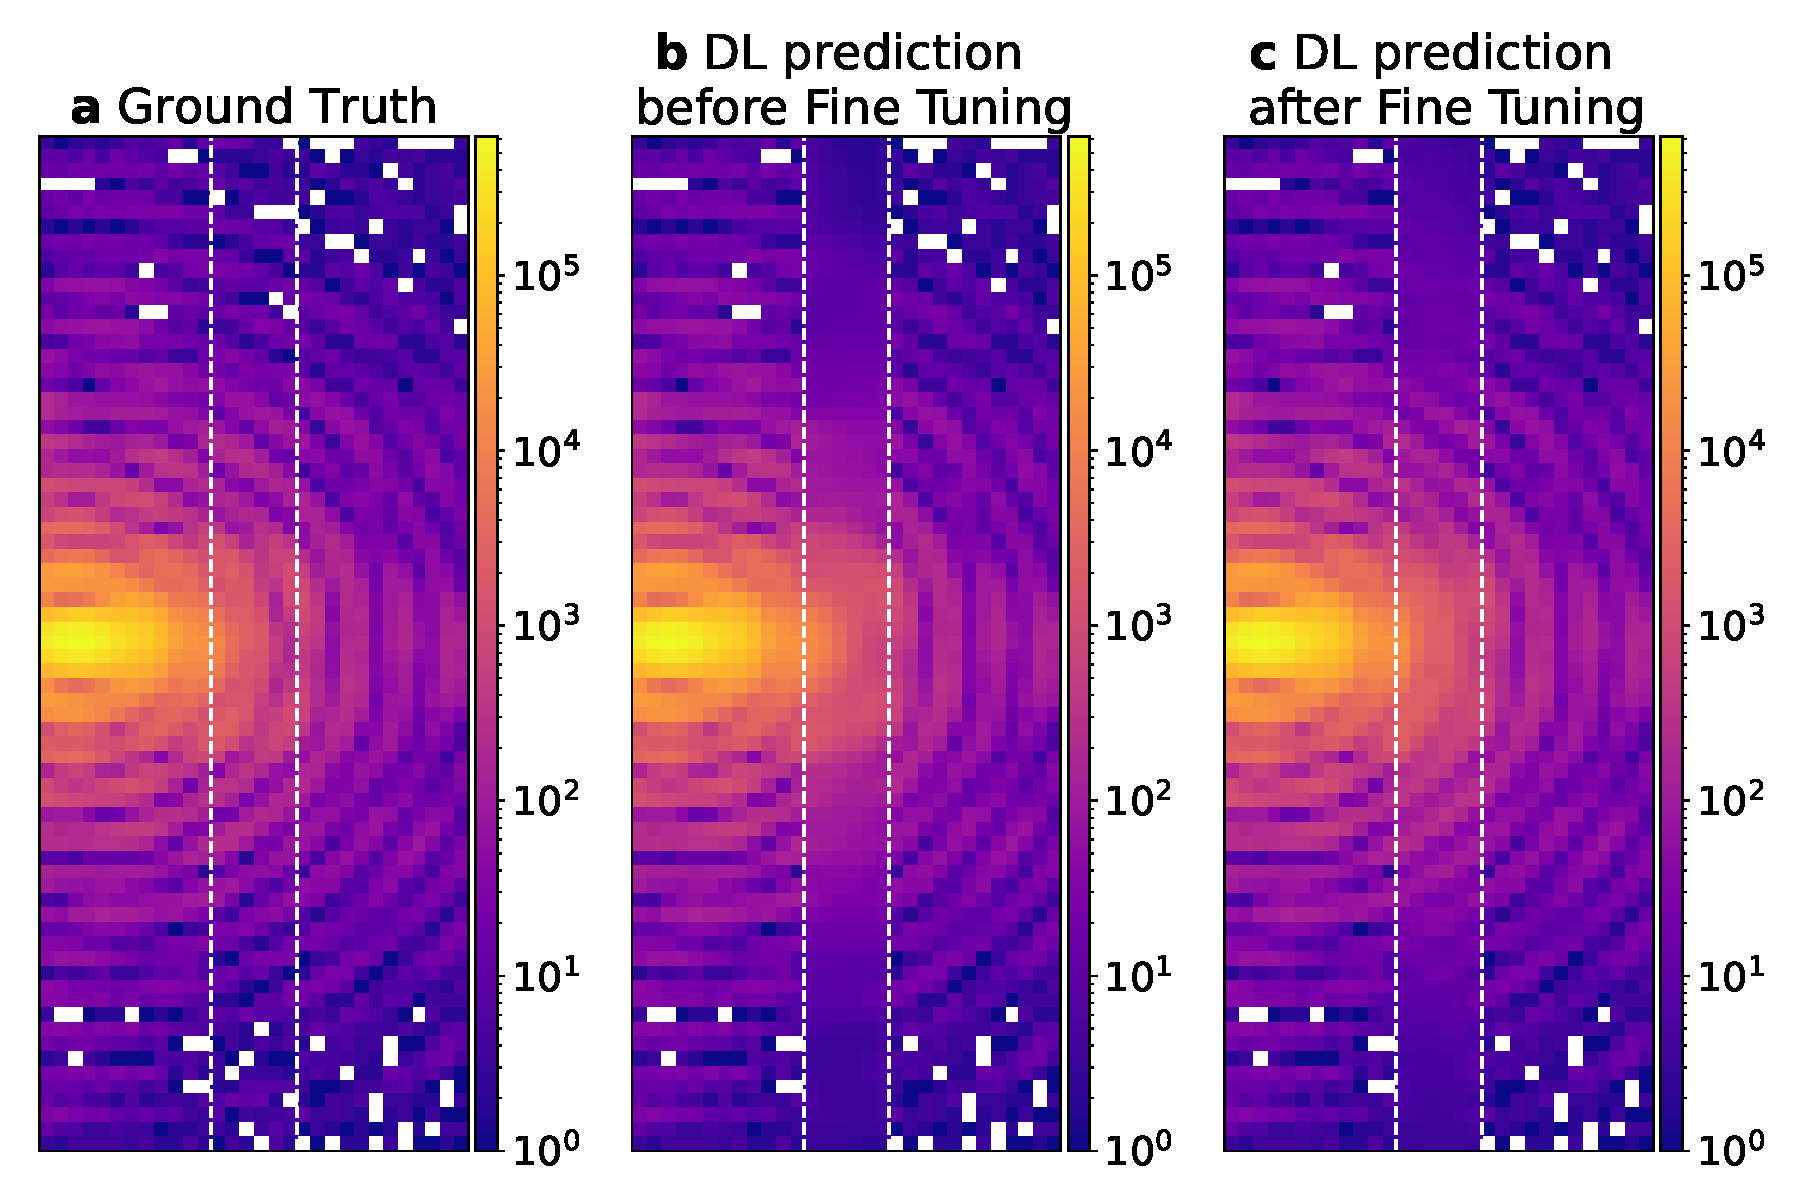
\includegraphics[width=\textwidth]{figures/Inpainting/FineTuning.pdf}
    \caption{\textbf{Example of improved accuracy after fine-tuning of the DL model on experimental data.} \textbf{a)} 
    The ground truth portion of the central slice of the BCDI experimental diffraction pattern. The dashed line 
    shows the position of the artificial 9 px-wide vertical gap applied for this test. \textbf{b)} Same slice 
    for the DL inpainted pattern \textit{before} fine-tuning. The fringes' periodicity is not recovered correctly. 
    \textbf{c)} Results \textit{after} fine-tuning. The fringes are now better recovered after 2 epochs of fine-tuning 
    on a dataset of 6400 patches cropped out of the same diffraction pattern (except the masked region). The fine-tuning 
    training took 110 seconds. }
    \label{fig:fine_tuning}
\end{figure}

The effect of the fine-tuning can also be assessed on the reconstructed object. Here, the diffraction patterns showed 
in Fig.\ref{fig:fine_tuning} has been phased with PyNX and the results are compared in Fig.\ref{fig:obj_fine_tuning}. 
For the phase retrieval, in all the three cases a single run of 400 HI0 + 1000 RAAR + 300 ER iterations has been performed starting 
from the autocorrelation of the object and with the shrinkwrap threshold of 0.2.  
As expected, already from visual inspection, the modulus and phase of the object reconstructed from BCDI pattern inpainted 
after the fine-tuning are more similar to the ground truth ones. On the contrary, the one obtained before the fine-tuning 
shows some oscillatory artifacts caused by the not correctly restored fringes. 

\begin{figure}[H]
    \centering
    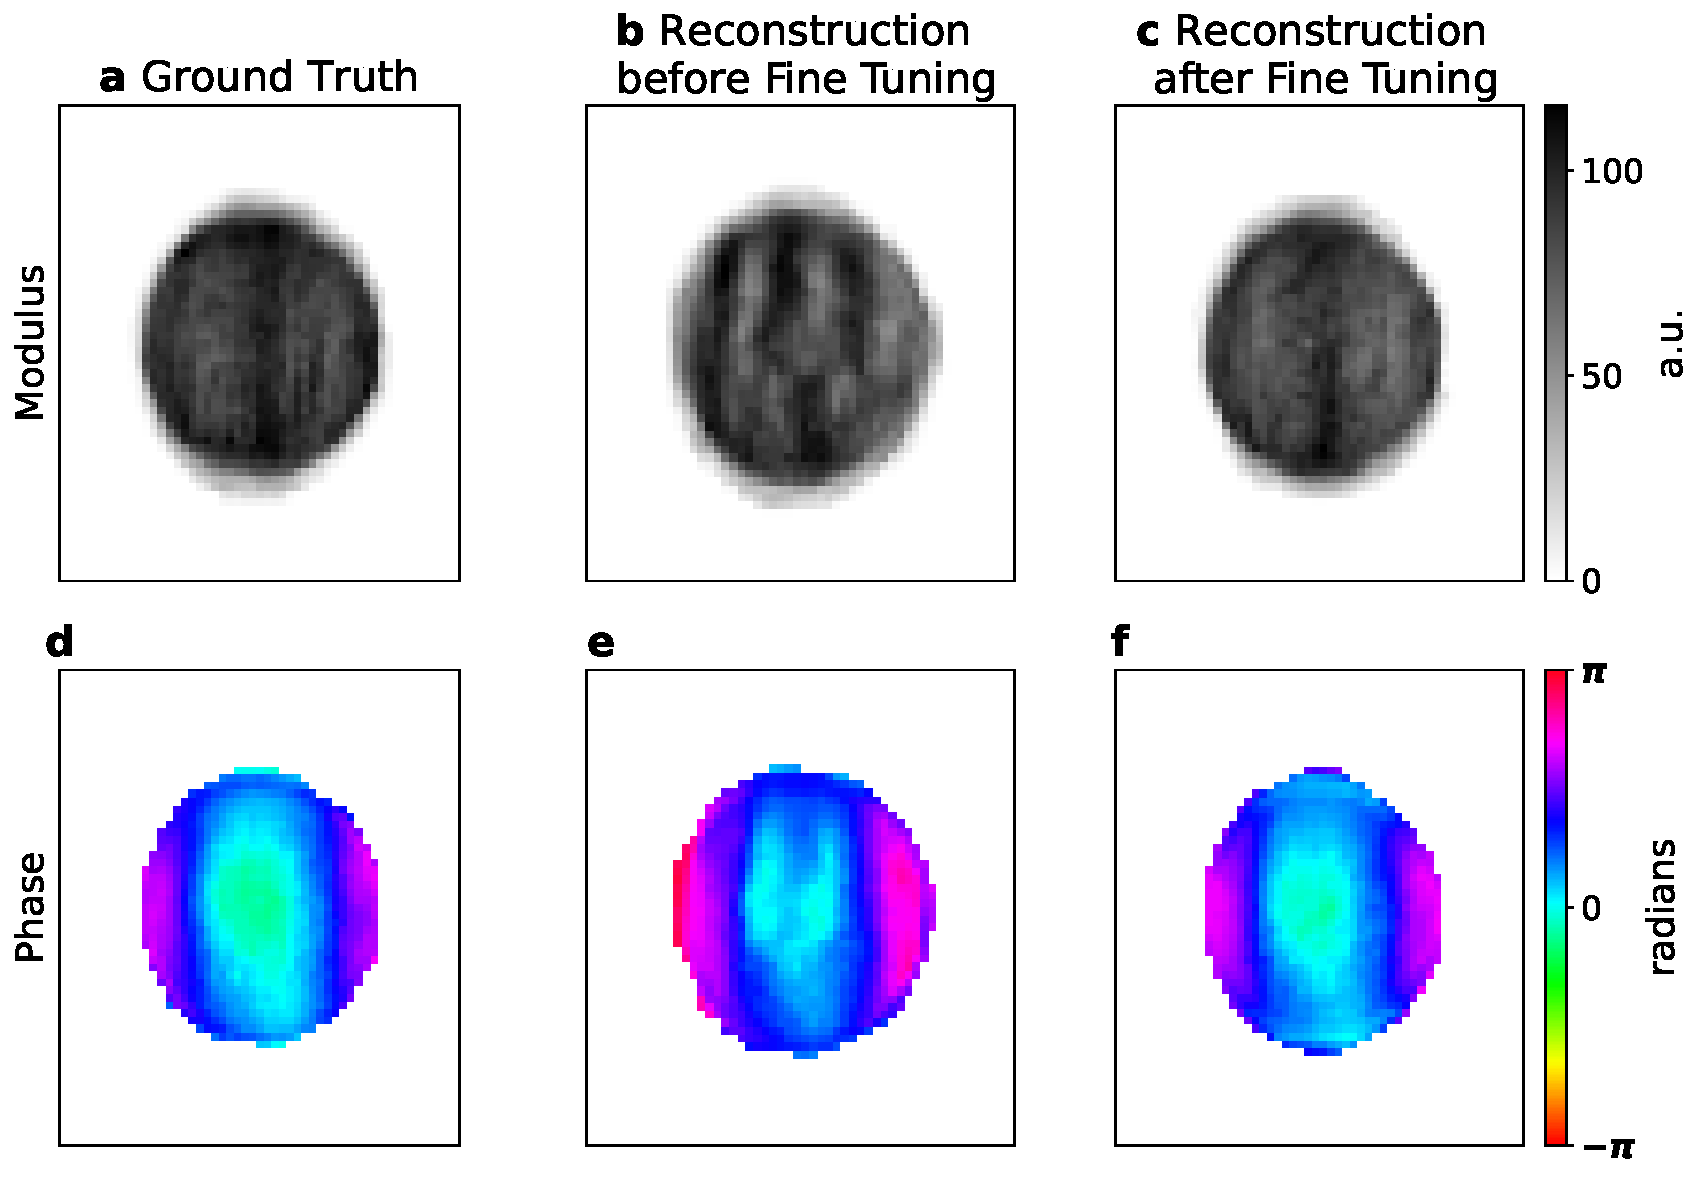
\includegraphics[width=\textwidth]{figures/Inpainting/obj_fine_tuning.pdf}
    \caption{\textbf{Reconstructed object before and after fine-tuning of the DL model} From the diffraction pattern in 
    Fig. \ref{fig:fine_tuning}, \textbf{a - d} Modulus and phase of the ground truth object. \textbf{b - e} and \textbf{c - f} 
    modulus and phase of the object reconstructed from the DL inpainted diffraction pattern \textit{before} and 
    \textit{after} fine-tuning respectively. The not well recovered fringes of Fig.\ref{fig:fine_tuning}\textbf{b} 
    produce artifacts in the reconstructed object that are eliminated with the inpainting of the fine-tuned DL model.
    }
    \label{fig:obj_fine_tuning}
\end{figure}
\section{Conclusions}

A novel DL model for the inpainting of BCDI patterns with detectors' gaps has been presented and tested for different 
experimental circumstances. The ``patching approach'' has proven to be adequate for BCDI for different reasons here summarized. 

\begin{itemize}
    \item Due to the oversampling condition, the BCDI patterns exhibit spatially regular and well-separated oscillations. 
    This local ``redundancy'' in detector space can be exploited by isolating smaller sub-volumes of the diffraction 
    pattern (\textit{patches}). In the presence of gaps, the missing signal within each patch can then be reconstructed 
    from neighboring voxels, with the reconstruction accuracy depending on the relative size of the gap compared to 
    the patch.

    \item The patching approach naturally allows for larger training datasets, faster training compared to full-image 
    direct inpainting approaches. Moreover, no lossy resizing is needed to adapt the whole BCDI pattern to the DL model size, as 
    in full-image direct inpainting. 

    \item DL inpainted experimental BCDI patterns have shown reduced artifacts in the reconstructed objects for different 
    gap-sizes, thus confirming improved reliability of the reconstructions. 

    \item Unlike full-image direct inpainting models the patching approach enables a model fine-tuning on each new specific 
    gap-affected dataset to be restored. This additional training can significantly improve the inpainting accuracy, 
    at the cost of only a few extra minutes of computation. 
        
\end{itemize}

The presented DL model is planned to be implemented in the PyNX package in the near future, such that it can be employed by 
a broader BCDI user community in standard data analysis pipelines. In these regards, it is worth mentioning that for 
an unbiased reconstruction, during the last iterations PR iterations, the 
inpainted pixels would need to be ``freed'' with a proper mask. In such a way, when the PR algorithm is near 
convergence, the data-fidelity is preserved. 

Future perspective can envision the extension of this patching approach to other CDI techniques. In the X-ray imaging 
community the detector gaps are in fact a common problem, as well as other limiting elements (beam-stops, defective pixels, 
overexposure, etc.). Given high-intensity signal covered by beam-stops and the higher accuracy of the DL model on 
bright patches, one could infer that CDI techniques like small-angle CDI and others in forward geometry could benefit 
from the presented DL inpainting approach.

